\documentclass[12pt,a4paper]{article}

\usepackage{graphicx}
\usepackage{pdfpages}
\graphicspath{{./figures/}}
\usepackage{subcaption}
\usepackage{amsmath}
\usepackage{booktabs}
\usepackage[footskip=0.2cm]{geometry}
\usepackage[english]{babel}
\usepackage{color}
\usepackage{float}
\usepackage{fancyhdr}
\usepackage{etoolbox}
\usepackage{hyperref}
\usepackage[sfdefault,lf]{carlito}

\usepackage{lipsum} % can be removed after you write your thesis

\usepackage{titlesec}
\titleformat*{\section}{\Huge\bfseries}

\renewcommand{\headrulewidth}{0pt}
\renewcommand{\footrulewidth}{1pt}

\usepackage{fancyhdr}
\usepackage{extramarks}

\setlength{\headheight}{14pt}

\begin{document}

% geometry settings for title page 
    \newgeometry{left=20mm, top=25mm, right=15mm, bottom=35mm}
% The title page settings can be changed in titlepage.tex document
    \begin{titlepage}
        \thispagestyle{fancy}
    \begin{figure}[H]
        \vspace{-1.5cm} % changes vertical spacing 
        \centering
        
\includegraphics[scale=1.05]{logo_unibo.png}
    \end{figure}
    
    \vspace{3mm}
    
    \begin{center}
        \bf {DEPARTMENT OF PHYSICS AND ASTRONOMY "A. RIGHI"}
    \end{center}
    
    \vspace{3mm}
    
    \begin{center}
        \bf \large{SECOND CYCLE DEGREE}
    \end{center}
    
    \vspace{0.7mm}
    
    \begin{center}
        \bf \large{PHYSICS}
    \end{center}
    
    \vspace{15mm}
    
    \begin{center}
        %
        % INSERT THE TITLE OF YOUR THESIS
        %
        {\huge{\bf Implementing a Digital Twin framework for Glioblastoma Patients}}
    \end{center}
    
    \vspace{50mm} \par \noindent
    
    \begin{minipage}[t]{0.47\textwidth}
        %
        % INSERT THE NAME OF THE SUPERVISOR WITH ITS TITLE (DR. OR PROF.)
        %
        {\large{\bf Supervisor \vspace{2mm}\\
        Prof. Gastone Castellani\\\\
        %
        % INSERT THE NAME OF THE CO-SUPERVISOR WITH ITS TITLE (DR. OR PROF.)
        %
        % IF THERE ARE NO CO-SUPERVISORS REMOVE THE FOLLOWING 5 LINES
        %
        \bf Co-supervisor %\textcolor{red}{optional}
        \vspace{2mm}\\
        Prof. Enrico Giamperi\\\\}}
    \end{minipage}
    %
    \hfill
    %
    \begin{minipage}[L]{0.40\textwidth} \textcolor{black}{
        {\large{\bf  Defended by
        \vspace{2mm}\\
        \noindent{Kasun Achintha Perera\\
        Podimarakkala Gurunnanselage}}}
        }
    \end{minipage}
    %
    \cfoot[C]{
        \\
        \bf Graduation Session / February/ 2027\\
        \vspace{3mm}
        \bf Academic Year 2026/2027
    }
    
\end{titlepage}

    \restoregeometry % goes back to default geometry

% if you don't need this page you can comment the lines contained between the ###
% ###
%\newpage
    %\thispagestyle{empty} 
    %\pagebreak
    %\hspace{0pt}
    %\vfill
    %\begin{flushright}
        %\textit{The important thing is not to stop questioning. Curiosity has its own reason for existing. One cannot help but be in awe when one contemplates the mysteries of eternity, of life, of the marvellous structure of reality. It is enough if one tries to comprehend only a little of this mystery every day.}\\
    
        %\vspace{0.3em}
        
        %\large{Albert Einstein}
    
    %\end{flushright}
    %\vfill
    %\hspace{0pt}
%\pagebreak
% ###

\pagenumbering{roman} % Sets page numbering to lower case roman numerals (i, ii, iii, ...)
\setcounter{page}{1} % Specifies the starting page numbe

\pagebreak
    \hspace{0pt}
    \vfill
    \addcontentsline{toc}{section}{Abstract}
    \section*{Abstract}
    
    Conventional neuro-oncological evaluation in Glioblastoma (GBM) care is primarily depending on static volumetric measurements and standardized response criteria to characterize prior tumor changes rather than forecast future tumor behavior. This study introduces the \texttt{NEXUS Brain Virtual Human Twin (VHT)} framework to bridge retrospective imaging analysis and prospective clinical decision making. The framework integrates longitudinal \texttt{NIfTI} segmentations, treatment exposure, and molecular context into a mechanistic, patient specific model of tumor growth and treatment response. An automated pipeline converted clinical and imaging repositories into structured digital patient records, retaining 155 of 203 patients (76.3\%) and yielding 546 longitudinal observations. A Hierarchical Bayesian Model (HBM), using non-centered parameterization and No-U-Turn Sampler (NUTS) \texttt{MCMC}, was formulated from the Fisher-KPP reaction diffusion equation, \(v_i=2\sqrt{D_i\rho_i}\). It simultaneously estimated population level hyperpriors and patient specific proliferation, diffusion, and carrying capacity parameters \((\rho_i,D_i,K_i)\), together with treatment efficacy coefficients for Chemotherapy, Radiotherapy, Immunotherapy, additional systemic therapies, and Brachytherapy. Calibrated parameters were deployed in a forecasting engine and interactive \texttt{Streamlit} dashboard for counterfactual scenario exploration. Cox proportional hazards models evaluated image derived kinetic features alongside \textit{IDH1}, \textit{MGMT} methylation, 1p/19q codeletion, age and etc. Convergence diagnostics showed \(\widehat{R}\leq1.04\), zero divergences, and \(\sigma_{\mathrm{obs},\log v}=0.8720\) (94\% HPD: 0.8190--0.9260). Patient specific parameters exhibited substantial heterogeneity with median proliferation was \(0.067\text{ day}^{-1}\), median diffusion \(0.434\text{ mm}^2/\text{day}\), and median wavefront speed \(0.086\text{ mm/day}\). Counterfactual simulations projected prospective tumor trajectories and evaluated multimodal interventions, including virtual resection and combined therapy windows, yielding substantial volume reductions. The VHT-driven Cox model produced a significant likelihood ratio test \((p=4.31\times10^{-7})\), identifying enhancing tumor velocity as a significant prognostic factor where one standard deviation increase was associated with an approximately 35.4\% higher mortality hazard. \textit{IDH1} mutation was protective. The \textsc{Nexus Brain} VHT framework translates longitudinal imaging into actionable growth projections and counterfactual simulations, demonstrating that dynamic image derived kinetics provide prognostic information beyond static baseline volumes and establishing a patient specific foundation for precision
    
    \vfill
    \hspace{0pt}
\pagebreak

\newpage

% Automatically creates Table of Contents
\tableofcontents
\newpage

% Automatically creates List of figures
\addcontentsline{toc}{section}{List of Figures}
\listoffigures
\newpage

% Automatically creates List of tables (remove these lines and \newpage if you don't have tables)
\addcontentsline{toc}{section}{List of Tables}
\listoftables
\newpage

% ###################################################################

\pagenumbering{arabic} % Sets page numbering to arabic (1, 2, 3, ...)
\setcounter{page}{1} % Specifies the starting page number

\pagestyle{fancy}
\fancyhead{}

\fancyheadoffset{0cm}
\renewcommand{\headrulewidth}{1pt} 
\renewcommand{\footrulewidth}{0pt}
\fancyhead[L]{{\thesection}}
\fancyhead[L]{\leftmark}

\section{Introduction}

\subsection{Clinical Motivation}

Glioblastoma (GBM) is the most common and the aggressive primary malignant brain tumor in adults age. Despite of maximal safe resection were followed by the radiotherapy and Temozolomide the prognosis remain poor with median overall survival approximately 14.6 to 21.1 months. Standard care consists maximal safe surgical resection where feasible followed by the focal Radiotherapy typically with "60 Gy" in "2 Gy" fractions with synchronous and post operative Temozolomide. \cite{brown2022survival}. Most patients still experience tumor recurrence and treatment decisions after the initial period remain uncertain yet this regimen improved survival relative to radiotherapy alone in the pivotal \texttt{EORTC}/\texttt{NCIC} trial. This is due to the diffuse infiltrative nature of GBM. Which means that tumor cells often extend beyond the abnormality visible on conventional MRI making complete surgical resection impossible and complicating both treatment planning and response assessment.\cite{singh2026digital}.

\begin{figure}[htbp]
    \centering
    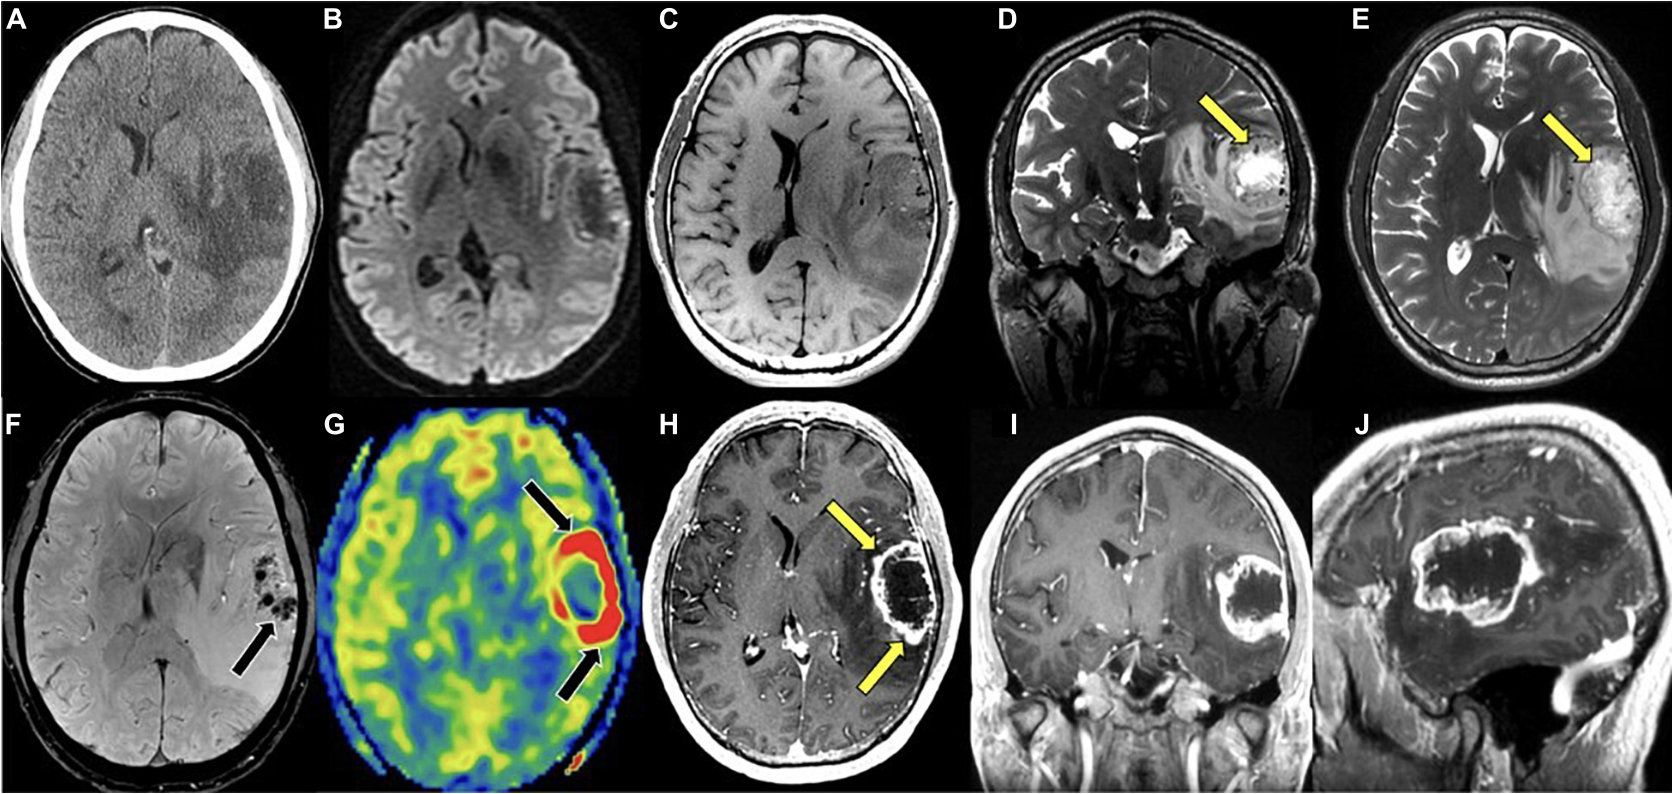
\includegraphics[width=0.85\textwidth]{figures/Figure Intro.png}
    \caption{Glioblastoma, IDH-wildtype multi parametric imaging characteristics. (A) Axial CT without contrast: ill-defined hypodensity lesion centered in the left superior temporal gyrus; (B) axial DWI: no associated reduced diffusion; (C) axial T1 pre contrast: hypointense mass; (D) coronal T2: heterogeneous mass with hypointense rim and prominent central necrosis (yellow arrow); (E) axial T2: heterogeneous mass with hypointense rim and prominent central necrosis (yellow arrow); (F) axial SWI: prominent blood products within the mass (black arrow); (G) axial ASL perfusion: marked hyperperfusion (black arrows) within the rim-enhancing component of the mass; (H) axial T1 post contrast: heterogeneous mass with thick rim enhancement (yellow arrows) and prominent central necrosis; (I) coronal T1 post contrast: heterogeneous mass with thick rim enhancement and prominent central necrosis; (J) sagittal T1 post contrast: heterogeneous mass with thick rim enhancement and prominent central necrosis. Abbreviations: CT, computed tomography; DWI, diffusion weighted imaging; SWI, susceptibility weighted imaging; ASL, arterial spin labeling; MRS, magnetic resonance spectroscopy. Adapted from \cite{carrete2022advanced}}.
    \label{fig:Glioblastoma_multimodal_imaging}
\end{figure}

Magnetic Resonance Imaging(MRI) is the base to every stage of GBM management including diagnosis, surgical 
planing, radiotherapy targeting, treatment response assessment and surveillance for recurrence. Multiparametric 
MRI particularly T1 Weighted(T1W) imaging before and after Gadolinium contrast administratiion, T2 Weighted(T2W) 
imaging and T2 Fluid Attenuated Inversion Recovery(T2-FLAIR) allows clinicians to visualize different tumor 
related compartments. In clinical practice segmentations and radiological assessments commonly distinguish by\cite{almeida2017advanced,FalkDelgado2025}:

\begin{itemize}
    \item \textbf{Necrotic core:} non enhancing central necrosis
    \item \textbf{Enhancing tumor:} contrast enhancing region suggestive of blood brain barrier disruption and active tumor related enhancement
    \item \textbf{Edema/infiltration:} T2-FLAIR hyperintensity that may represent vasogenic edema, infiltrative tumor, or both
    \item \textbf{Resection cavity:} the post surgical cavity and surrounding treatment related changes
\end{itemize}

Longitudinal MRI is specially important after the treatments because changes over time can provide more informative evidence than a single scan. An increase in enhancing volume, new enhancement or increasing T2-FLAIR abnormality may suggest progression but it may also reflect treatment related inflammation, ischemia or radiation injury. Therefore the clinical interpretation of MRI is inherently longitudinal. The same finding can have different implications depending on its timing relative to surgery, Radiotherapy, Chemotherapy and prior imaging.\cite{ellingson2017pseudoprogression}

\subsection{The Pseudoprogression problem}

So after the treatments, serial MRI is used as the principal tool for assessing tumor control, progression and the treatment related injury. However conventional MRI cannot always distinguish true tumor progression from the pseudoprogression or radiation necrosis. Because all of these changes can produce contrast enhancement or T2/FLAIR signal variations.\cite{barajas2019pseudoprogression}. Further more, Pseudoprogression refers to a new enlarging area of contrast enhancement that occurs in the absence of true tumor growth and subsequently stabilize or resolves without a change in therapy. It is thought to reflect treatment induced inflammatory changes, vascular permeability and blood brain barrier disruption rather than proliferating tumor. Radiation necrosis is related but typically later occurring treatment effect can also mimic recurrent tumor on conventional MRI. This distraction is difficult because of pseudoprogression. Radiation necrosis and true progression can all increaing contrast enhancement, mass effect, peritumoral edema and worsening the neurological symptoms.\cite{thust2018pseudoprogression}.

\begin{figure}[htbp]
    \centering
    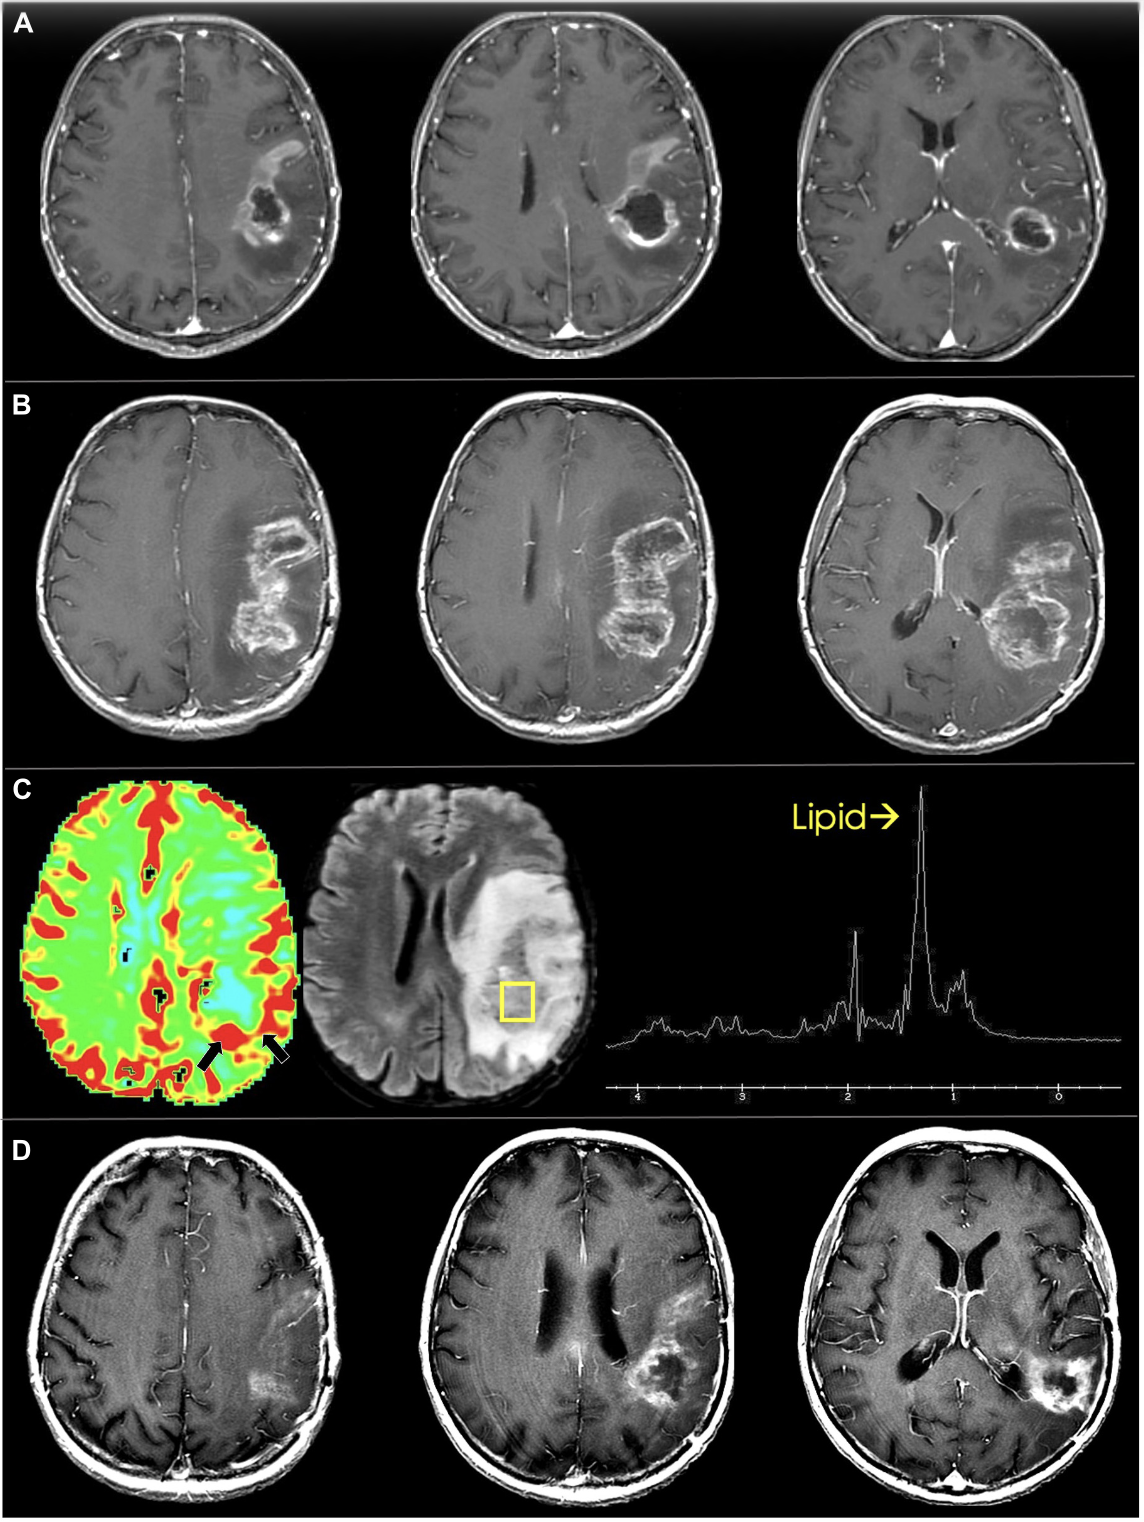
\includegraphics[width=0.85\textwidth]{figures/Figure Pseudoprogression.png}
    \caption{Pseudoprogression in Glioblastoma. (A) Immediate pre Radiotherapy: axial T1 post contrast images show rim enhancing and centrally necrotic left frontoparietal Glioblastoma; (B) Eight week follow-up: immediate post Radiotherapy axial T1 post contrast images show marked increase in enhancement and necrosis; (C) dynamic susceptibility weighted contrast enhanced perfusion MRI shows mild increase in blood volume along the posterior rim (black arrows), while single voxel proton spectroscopy targeted to the posterior component shows a markedly increased lipid peak suggesting tissue necrosis; (D) Three month follow up: axial T1 contrast images show marked decrease in enhancement and necrosis of the treated Glioblastoma. Adapted from \cite{carrete2022advanced}.}
    \label{fig:glioblastoma_pseudoprogression}
\end{figure}

This doubtfulness is clinically consequential. A patient with pseudoprogression may be incorrectly considered to have progressive disease, whereas a patient with true progression may experience delayed escalation of therapy. Current reviews emphasize that conventional MRI alone is often insufficient and histopathology remains the reference standard in ambiguous cases.\cite{tran2013treatment}. The clinical consequences of this uncertainty are substantial:

\begin{itemize}
    \item A patient with pseudoprogression may be incorrectly classified as having progressive disease, potentially leading to premature discontinuation of effective therapy or unnecessary escalation.
    \item A patient with true progression may have treatment escalation delayed while awaiting confirmatory imaging.
    \item Repeated imaging, advanced MRI, positron emission tomography, or tissue sampling may be required, increasing cost, delay, patient burden, and diagnostic uncertainty.
\end{itemize}

Advanced imaging techniques including perfusion MRI, Diffusion Weighted Imaging, Magnetic Resonance Spectroscopy and Amino Acid \texttt{PET} can provide additional information. However even these modalities do not always provide a definitive distinction between pseudoprogression and true progression.\cite{delgado2018treatment}.

\subsection{The need for the longitudinal interpretation}

Current response assessment frameworks including the Response Assessment in Neuro Oncology(RANO) criteria recognize that interpretation must account the treatment time. RANO 2.0 specially highlights the pseudoprogression is frequent during the first 12 weeks after the Radiotherapy. During this period, progression generally requires confirmation by repeat MRI or histopathological evidences of recurrent tumor. Therefore a Digital Twin (DT) should not simply interpret an increase in enhancing volume as progression. It should incorporate scan timing, treatment exposure, molecular context and longitudinal trajectory.\cite{wen2023rano20}.

\begin{figure}[htbp]
    \centering
    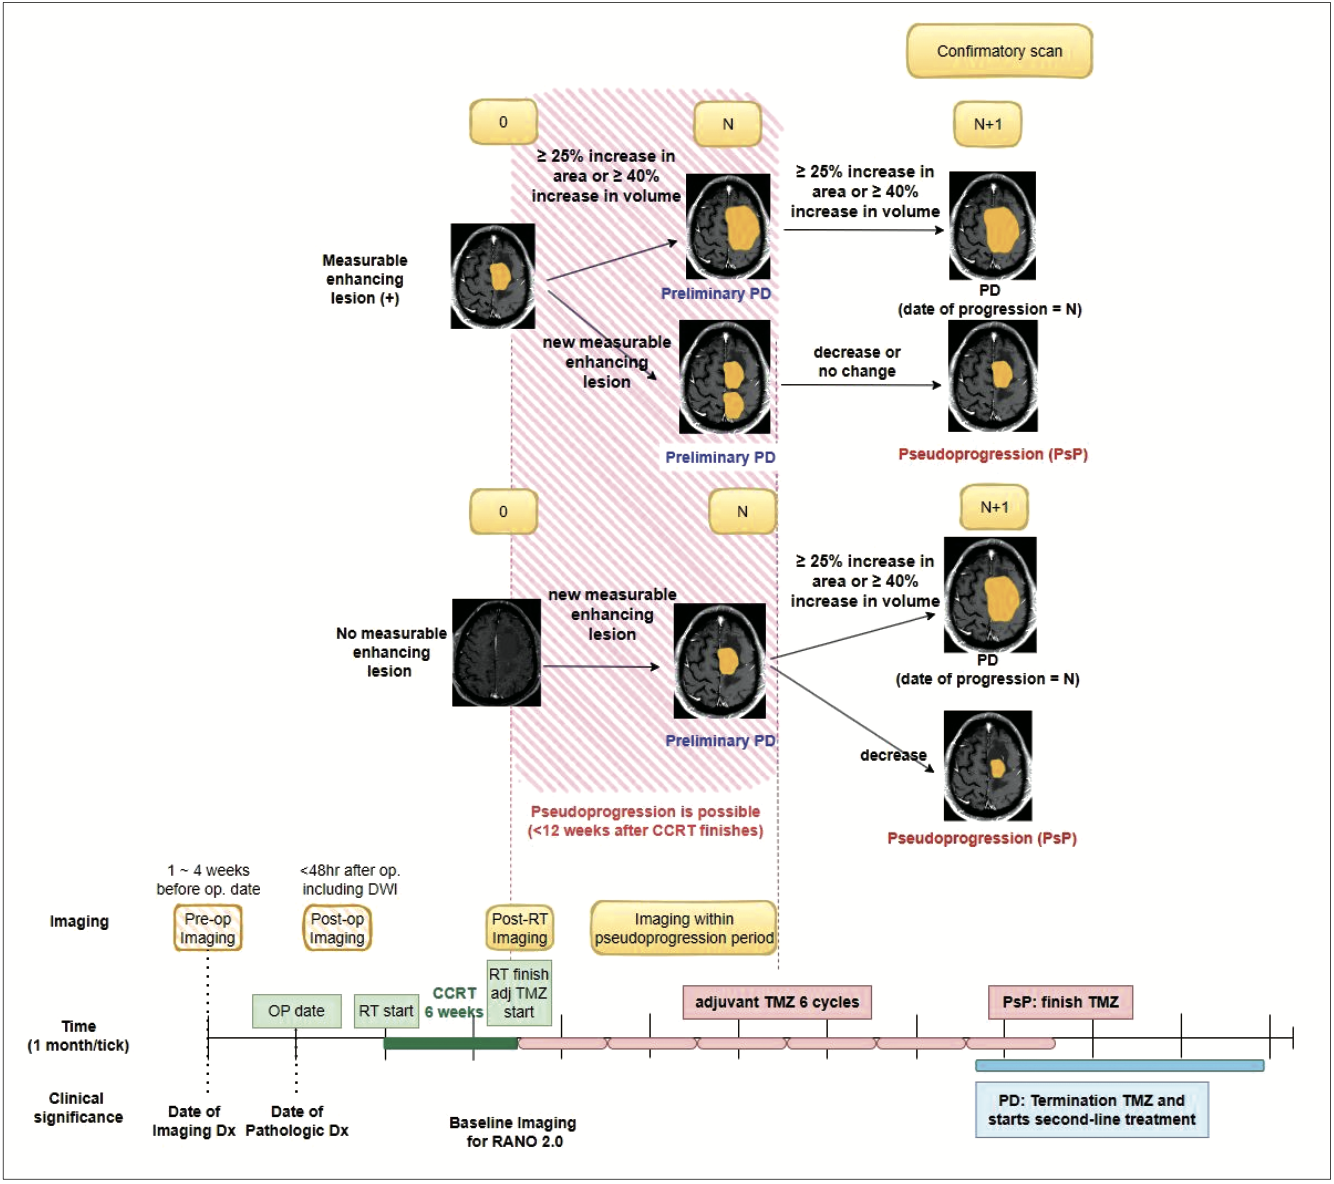
\includegraphics[width=1.00\textwidth]{figures/Figure RANO.png}
    \caption{Longitudinal response assessment according to the Response Assessment in 
    Neuro-Oncology (RANO) 2.0 criteria. In newly diagnosed Glioblastoma, the post Radiotherapy 
    MRI is used as the baseline for subsequent response assessment. Because pseudoprogression 
    is frequent during the first 12 weeks after completion of radiotherapy or concurrent 
    chemoradiotherapy, apparent progression during this period requires confirmation by repeat 
    MRI or histopathological evidence of unequivocal recurrent tumor before progressive disease 
    is declared. This temporal framework highlights the importance of incorporating scan timing, 
    treatment exposure, and serial imaging trajectories into computational models of tumor 
    dynamics. Adapted from \cite{sakata2024rano}.}
    \label{fig:rano2_pseudoprogression_timeline}
\end{figure}

This has two important implications for computational modeling. First a model that interprets an increase in enhancing tumor volume as tumor growth without considering the time since, Radiotherapy may misclassify treatment related inflammation as progress. Early post treatment enhancing expansion should therefore be interpreted in the context of Radiotherapy completion date, Chemotherapy exposure steroid use and subsequent imaging trajectory. Secondly a single MRI timepoint provides limited information about tumor dynamics. The rate of change in tumor volume, enhancing tissue, edema and imaging heterogeneity may be more informative than any individual measurement. Longitudinal features such as volume velocity, voxel count velocity, intensity change and heterogenity change can capture temporal behavior that is invisible in a static scan. \cite{sakata2025rano}.

\subsection{Molecular heterogeneity and personalized care}

\begin{figure}[htbp]
    \centering
    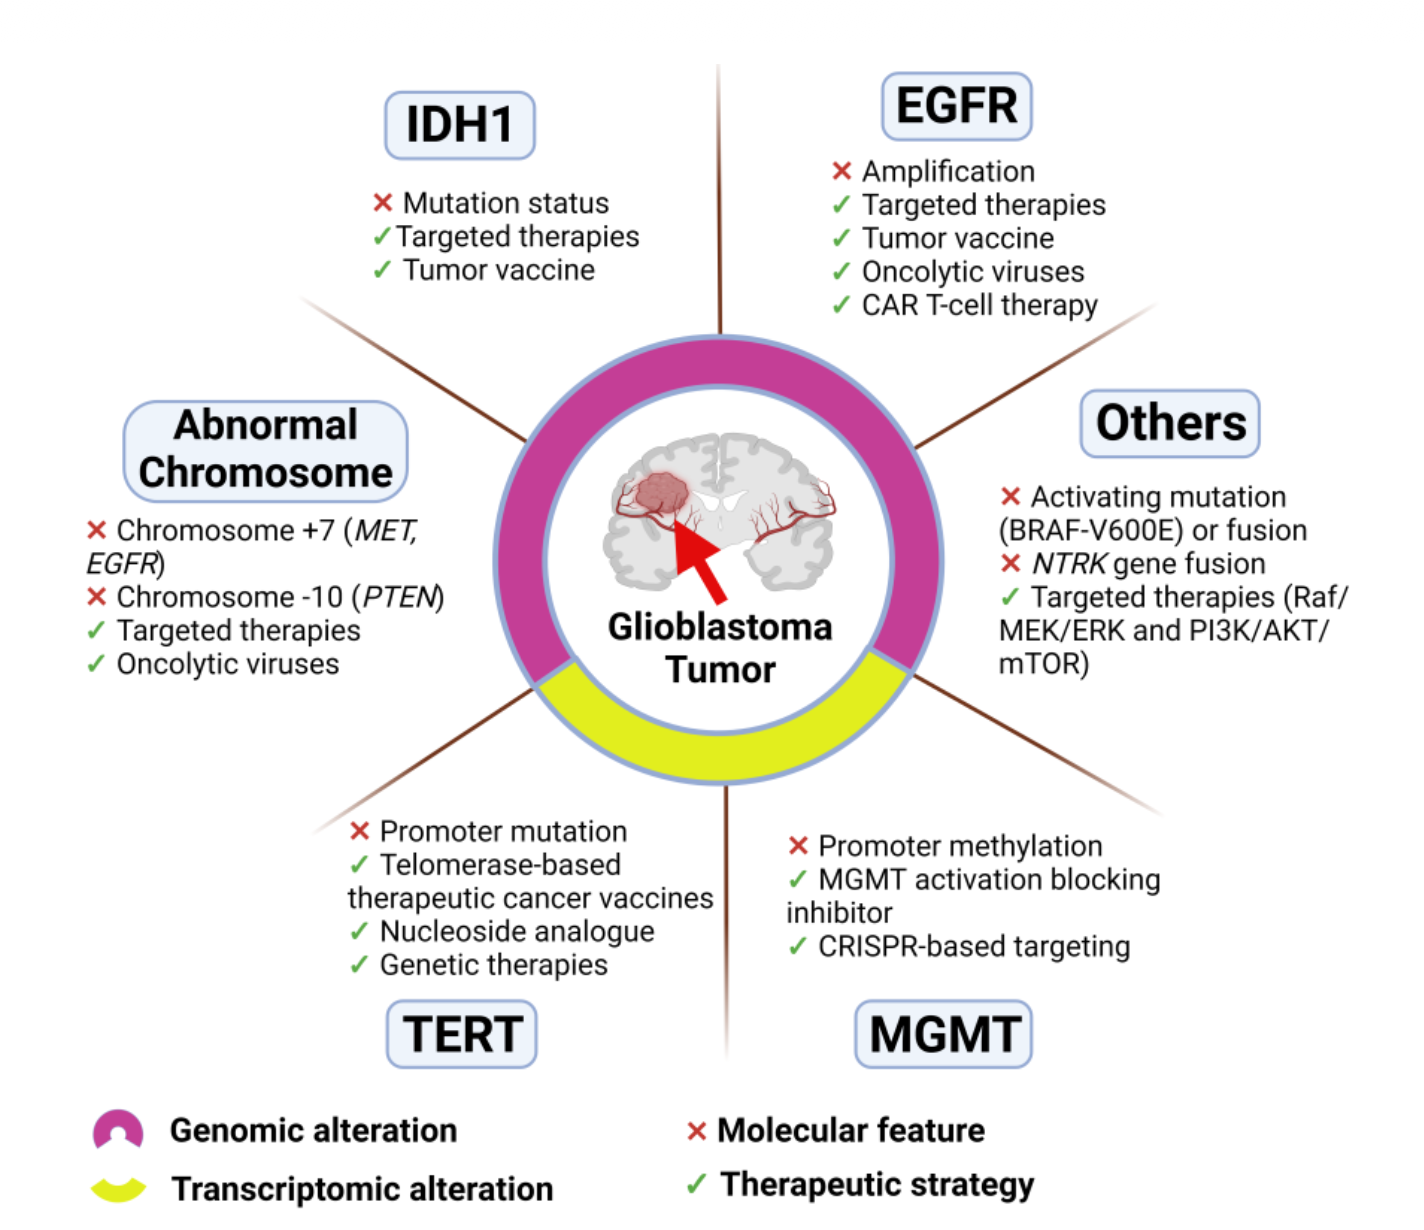
\includegraphics[width=0.85\textwidth]{figures/Figure Molecular Hetoregeneity.png}
    \caption{Molecular heterogeneity in Glioblastoma. Molecular alterations, including \textit{IDH} mutation status, \textit{MGMT} promoter Methylation, \textit{TERT} promoter mutation, \textit{EGFR} amplification, \textit{PTEN} alteration, \textit{CDKN2A/B} deletion, and \textit{TP53} alteration, influence prognosis, treatment sensitivity, and expected tumor behavior. \textit{IDH}-mutant Gliomas generally have a more favorable prognosis than \textit{IDH}-wildtype tumors, whereas \textit{MGMT} promoter methylation is associated with greater temozolomide sensitivity and improved survival. These molecular features provide important biological context for interpreting apparently similar MRI phenotypes and for personalizing computational models of tumor growth and treatment response. Adapted from \cite{zhu2024molecular}.}
    \label{fig:gbm_molecular_heterogeneity}
\end{figure}

Glioblastoma is not a biologically uniform disease. Molecular features strongly influence prognosis, treatment sensitivity, and expected tumor behavior. Molecular markers such as \texttt{IDH} mutation, \texttt{MGMT} promoter Methylation, \texttt{1p/19q} codeletion, \texttt{TERT }promoter mutation, \texttt{EGFR} amplification, \texttt{PTEN} alteration, \texttt{CDKN2A/B} deletion, and \texttt{TP53} alteration are established prognostic and predictive factors. Meta analytic evidence support their positive prognostic significance across treatment types.\cite{karsy2015practical}. 

\texttt{IDH} mutant Glioma generally have a more favorable prognosis than \texttt{IDH} wildtype tumors, whereas \texttt{IDH} wildtype GBM tends to behave more aggressively. \texttt{MGMT} promoter methylation is both prognostic and predictive. MGMT methylation was significantly associated with better overall survival, with a pooled hazard ratio of 1.66 for unmethylated versus methylated status.\cite{noroxe2016hallmarks}. Also \texttt{MGMT} promoter Methylation is associated with greater sensitivity to Temozolomide and longer survival. In \texttt{IDH} wildtype Glioblastoma, methylated \texttt{MGMT} has been associated with a median overall survival of approximately 24 months, compared with approximately 14 months in unmethylated tumors.\cite{melhem2022updates}.

These variables should therefore not be treated as optional metadata. They provide biological context that may help to explain why two patients with similar MRI appearances can have very different growth rates, treatment responses and survival outcome.

\subsection{Limitations of current decision support and Digital twins as a potential solution}

At present clinical decision making commonly relies on visual interpretation of serial MRI, volumetric or bidimensional RANO measurements, clinical symptoms and corticosteroid use, molecular markers and multidisciplinary tumor board discussions. These sources of information are essential but they are often assessed separately. Imaging findings may not be explicitly linked to the patients treatment timeline, molecular profile and longitudinal outcome trajectory. Furthermore conventional assessments provides limited formal quantification of uncertainty. Clinicians may recognize that a finding of uncertain but they rarely receive a calibrated estimate of probability that a given trajectory represents progression versus treatment effect. This creates a need for a framework that can integrate heterogeneous patient specific data into a coherent, quantitative representation of tumor behavior\cite{luemerson2026corticosteroids}.

A Digital Twin(DT) is a patient specific computational representation that integrates clinical, imaging, molecular and treatment data to simulate disease behavior and support decision making. In oncology Digital Twin(DT)s can combine observed patient data with mechanistic models to estimate hidden biological processes, forecast future disease trajectory and quantify uncertainty. For Glioblastoma, a digital twin could integrate:

\begin{itemize}
    \item Serial MRI derived tumor volumes
    \item Tumor compartment segmentations
    \item Intensity and heterogeneity features
    \item Molecular biomarkers
    \item Treatment timing and exposure
    \item Clinical outcomes such as progression free survival and overall survival
\end{itemize}

Reaction diffusion models are particularly suitable for this purpose because they represent two central processes of Glioblastoma biology. Local proliferation and diffusion driven invasion into surrounding brain tissue. When personalized with imaging data, these models can estimate tumor dynamics beyond the visible enhancing margin and may predict infiltrative growth not directly captured by MRI.


\begin{equation}
    \frac{\partial N(x,t)}{\partial t} = D \nabla^2 N(x,t) + \rho N(x,t)\left(1 - \frac{N(x,t)}{K}\right) - R(N,t),
    \label{eq:fisher_kpp_custom}
\end{equation}

Fisher–KPP reaction diffusion model provides a compact mathematical representation of these processes. where $N(x,t)$ is the tumor cell density, while $D$ represents the invasion/diffusion, $\rho$ represents proliferation, then $K$ is the carrying capacity, and $R(N,t)$ represents the treatment induced cell kill or growth inhibition. \cite{fritz2025timefractional}.

By calibrating such a model to a patient specific serial MRI derived tumor volumes helps to estimate parameters such as rate of proliferation and spacial invasion, that are not directly observable from a single scan. This patient specific reaction diffusion approaches including physics informed neural network(PINN) methods have been developed to infer Glioblastoma infiltration parameters from structural MRI.

\subsection{Clinical value of the proposed Digital Twin}

A patient linked Digital Twin could support clinical decision making in several ways:

\begin{itemize}
    \item \textbf{Earlier risk stratification:} identify patients whose estimated proliferation or invasion rates suggest higher risk of progression.
    \item \textbf{Longitudinal interpretation:} place a new MRI finding in the context of the patient's prior trajectory and treatment timeline.
    \item \textbf{Pseudoprogression-aware monitoring:} avoid overinterpreting early post-radiotherapy enhancement by incorporating time since treatment and subsequent imaging evolution.
    \item \textbf{Personalized forecasting:} estimate future tumor burden with uncertainty intervals rather than providing a single deterministic prediction.
    \item \textbf{Treatment-scenario exploration:} simulate how alternative treatment assumptions might affect predicted tumor dynamics.
    \item \textbf{Decision support:} provide clinicians with an additional quantitative tool alongside RANO assessment, clinical examination, and multidisciplinary review.
\end{itemize}

The objective is not to replace clinical judgement or RANO criteria. The Digital Twin would complement RANO assessment, clinical examination, molecular diagnostic and multidisciplinary review by providing a quantitative  patient specific and uncertainty aware representation of tumor behavior.

\subsection{Research Motivation}

Despite growing interest in Digital twin for neuro oncology, major challenges remain. Many existing models are developed using single snapshot imaging data, do not incorporate treatment timing, or do not explicitly link model derived tumor dynamics to longitudinal clinical outcomes. In addition, imaging, molecular, treatment and survival data re often stored in separated formats and analyzed independently and limiting their usefulness for patient specific modeling.

This project addresses these limitations by developing a patient linked Digital Twin framework for Glioblastoma. The framework integrates longitudinal MRI derived tumor measurements, Radiomic descriptors, molecular priors, treatment exposure and survival outcomes with a unified computational pipeline. By calibrating a Fisher KPP based tumor growth model to patient specific longitudinal data the proposed Digital Twin aims to estimate individual tumor dynamics, forecast future tumor burden with uncertainty and explore associations between model derived dynamics and clinical outcomes.

Ultimately the goal is to move beyond static population level prediction toward a reproducible patient specific framework that can support more informed and personalized decision making in Glioblastoma care.



\newpage

\section{Methodology and Pipeline Structure}

\subsection{Pipeline Architecture}

\begin{figure}[htbp]
    \centering
    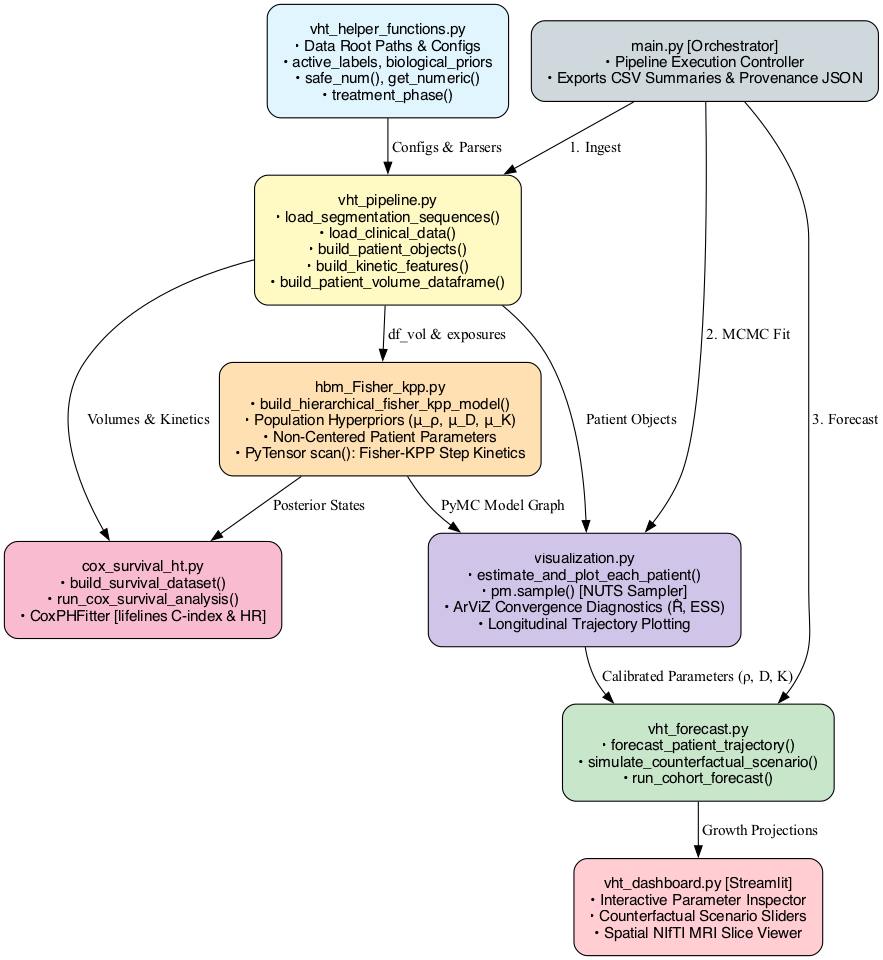
\includegraphics[width=0.85\textwidth]{figures/system_structure.png}
    \caption{Comprehensive structural architecture and module interaction flow of the NEXUS Brain Virtual Health Twin (VHT) framework.}
    \label{fig:system_structure}
\end{figure}

The \textsc{Nexus Brain} Virtual Health Twin (VHT) framework establishes an end to end computational pipeline for patient specific modeling of Glioblastoma progression. It integrates longitudinal Neuroimaging segmentations, multi center clinical histories, Radiobiological treatment parameters, and molecular biomarkers into a unified analytical workflow. The pipeline ingests multimodal MRI scans and clinical records through \texttt{vht\_pipeline.py}, extracting longitudinal tumor volumes, volumetric changes, and treatment exposure fractions. Rather than representing therapies as binary exposures, the framework quantifies the proportion of each inter scan interval during which Chemotherapy, Radiotherapy, Immunotherapy, additional therapies, or Brachytherapy was active.

These longitudinal imaging and treatment features are used to calibrate a Hierarchical Bayesian Model (HBM) implemented with \texttt{PyMC} and \texttt{PyTensor} in \texttt{hbm\_Fisher\_kpp.py}. The model is based on the Fisher-KPP Reaction Diffusion equation and estimates patient specific proliferation (\(\rho\)), diffusion (\(D\)), carrying capacity (\(K\)), and treatment efficacy coefficients (\(\alpha_m\)). The hierarchical structure enables the framework to capture both cohort level tumor growth patterns and individual deviations, allowing tumor dynamics of each patient to be represented by calibrated parameters informed by their own longitudinal data.

The calibrated parameters are subsequently passed to a forecasting and counterfactual simulation module, \texttt{vht\_forecast.py}. This module projects future tumor growth from the most recent available scan and evaluates hypothetical clinical scenarios by including surgical resection, altered treatment timing, and multi modal therapy schedules. Furthermore, by comparing projected trajectories under different assumptions, the framework supports “what-if” analyses of interventions that were not observed in the original clinical course.

The framework also provides interactive clinical exploration through a \texttt{Streamlit} dashboard, \texttt{vht\_dashboard.py}. The dashboard enables selection of individual patients, inspection of calibrated growth parameters and historical tumor volumes, configuration of virtual treatment scenarios, and visualization of projected tumor trajectories alongside longitudinal MRI data. Finally, \texttt{cox\_survival\_ht.py} links model derived tumor kinetics, treatment exposures, and genetic biomarkers to survival outcomes using regularized Cox proportional hazards modeling. Automated provenance logging through \texttt{run\_metadata.json} records key execution details, supporting transparency, reproducibility, and computational auditability across the full pipeline.





\subsection{Shared Configuration and Utility Functions (\texttt{vht\_helper\_functions.py})}

\begin{figure}[htbp]
    \centering
    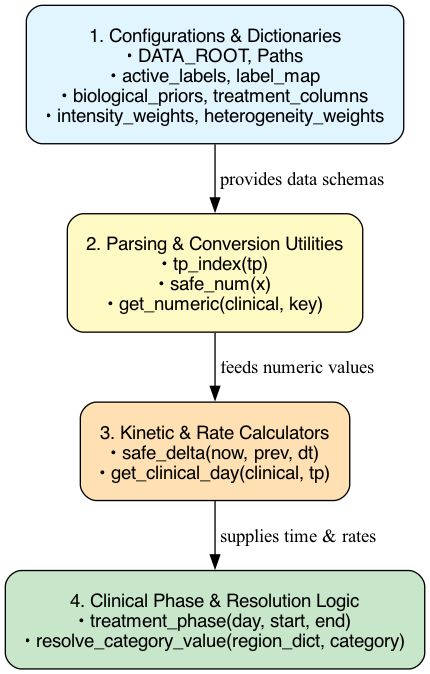
\includegraphics[width=0.35\textwidth]{figures/helper_functions_structure.png}
    \caption{Comprehensive structural architecture and module interaction flow of the NEXUS Brain Virtual Health Twin (VHT) framework.}
    \label{fig:helper_function_structure}
\end{figure}

The \texttt{vht\_helper\_functions.py} module provides the shared configuration, data mappings, and utility functions used throughout the \texttt{Nexus Brain} VHT pipeline. It standardizes the interpretation of raw clinical, imaging, and segmentation data before feature extraction, Bayesian calibration, forecasting, and survival modeling. By centralizing these operations, the module ensures consistent handling of tumor labels, clinical variables, treatment intervals, and derived imaging features. The module defines the locations of the primary data sources, including the MRI image directory, segmentation volume spreadsheet, and clinical data spreadsheet. It also specifies the clinical worksheet containing patient level records. Centralizing these paths ensures that downstream modules access the same source data and reduces the risk of inconsistent file handling.

Segmentation labels are harmonized into four biologically meaningful tumor compartments: necrotic core, enhancing tumor, edema, and resection cavity. Raw labels, such as "Necrotic Tumor Core (Label1)" and "Tumor Infiltration and Edema," are mapped to standardized categories. This harmonization is necessary because source data may use different naming conventions, while downstream modeling requires a consistent set of tumor subregions. Then module defines biological priors and treatment related clinical variables. Biological priors include established Glioblastoma associated molecular and genetic markers, such as \textit{IDH1} and \textit{IDH2} mutation, \textit{MGMT} promoter Methylation, \textit{1p/19q} codeletion, \textit{ATRX} mutation, \textit{TERT} promoter mutation, \textit{EGFR} amplification, \textit{PTEN} mutation, \textit{CDKN2A/B} deletion, \textit{TP53} alteration, and tumor grade. These variables are retained for downstream survival modeling and will be used to assess associations between molecular features, tumor kinetics, and clinical outcomes.

Treatment variables capture the type, timing, dose, and duration of Chemotherapy, Radiotherapy, additional systemic therapies, Immunotherapy, and Brachytherapy. Also this module defines paired Start and End day fields for each treatment type and allow the pipeline to construct treatment intervals relative to the date of diagnosis. It is essential for calculating treatment exposure during each MRI interval. Furthermore, this module defines modality specific weights for calculating composite intensity and heterogeneity features within each tumor compartment. Four MRI sequences are considered: contrast enhanced T1 weighted imaging (T1C), non contrast T1 weighted imaging (T1N), T2-FLAIR (T2F), and T2 weighted imaging (T2W). The weights reflect the expected relative contribution of each sequence to the biological interpretation of a given tumor region. For example, enhancing tumor regions are weighted most heavily toward T1C signal, because contrast enhancement is primarily associated with blood brain barrier disruption and active tumor tissue\cite{fan2024radiomics}. In contrast, edema is weighted more strongly toward T2-FLAIR and T2-weighted sequences, which are more sensitive to vasogenic edema and infiltrative change. Similar region-specific weighting is applied to heterogeneity features, enabling standardized measures of signal intensity and intratumoral variability across MRI sequences.

Several helper functions standardize the extraction of numeric values from heterogeneous clinical data. The \texttt{safe\_num()} function converts numeric values, numeric strings, and strings containing embedded numbers into floating point values. For example, a dose recorded as "60 Gy" or a fraction count recorded as "30 fractions" can be converted to 60.0 and 30.0, respectively. Missing, non numeric, or malformed entries are returned as \texttt{NaN}, preventing invalid values from entering the modeling pipeline. The \texttt{get\_numeric()} function extends this behavior for clinical metadata dictionaries. It performs robust key matching, removes unnecessary whitespace, recognizes common missing value labels such as "NA", "N/A" and "NONE", and extracts the first numeric value from mixed text number fields. This is particularly important for multi center clinical datasets, where the same variable may be recorded using different formats or units.

The \texttt{safe\_delta()} function calculates the rate of change of a variable between consecutive time points. It divides the difference between the current and previous value by the elapsed time while explicitly handling missing values and non positive time intervals. This function is used to derive features such as tumor volume velocity, voxel count velocity, and changes in image derived intensity or heterogeneity measures. The \texttt{get\_clinical\_day()} function maps each imaging time point to its corresponding number of days from diagnosis. It identifies clinical fields containing the relevant time point identifier and converts the associated value to a numeric day. This enables alignment of MRI derived tumor measurements with treatment windows and supports calculation of inter-scan time intervals.

The \texttt{treatment\_phase()} function classifies each imaging time point relative to a treatment interval. A scan occurring before the treatment start date is labeled "pre", a scan within the treatment window is labeled "active", and a scan after treatment completion is labeled "post". If treatment start or end information is unavailable, the function returns ``none'' or applies a defined fallback rule. This classification supports the construction of treatment phase indicator variables for use in kinetic modeling, counterfactual simulation, and survival analysis. Finally, \texttt{resolve\_category\_value()} retrieves tumor compartment values from dictionaries containing raw segmentation labels. It uses case insensitive substring matching to identify the appropriate region, with special handling for edema related labels which may include terms such as "infiltration". This function ensures that standardized categories such as "Necrotic", "Enhancing", "Edema", and "Resection" can be reliably mapped back to their original segmentation volume entries.

Overall, \texttt{vht\_helper\_functions.py} acts as the data standardization and feature engineering foundation of the \textsc{Nexus Brain} VHT framework. It converts heterogeneous clinical records and segmentation outputs into clean, consistently structured numerical features suitable for longitudinal modeling. This module ensures that tumor kinetics, treatment exposure, Bayesian calibration, counterfactual simulation, and survival analysis are based on a common and reproducible data representation by defining shared label mappings, treatment intervals, imaging weights, and robust parsing functions.


\subsection{Digital Patient Construction and Feature Engineering (\texttt{vht\_pipeline.py})}

\begin{figure}[htbp]
    \centering
    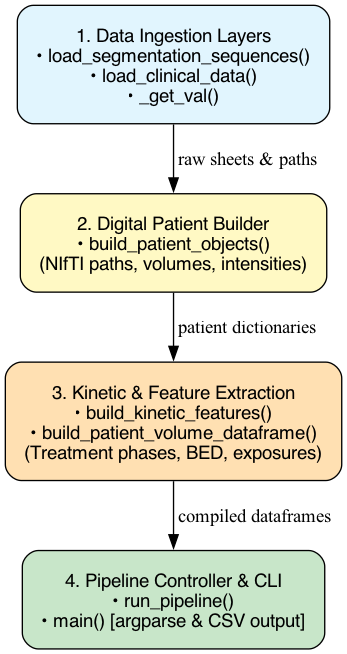
\includegraphics[width=0.35\textwidth]{figures/pipeline_structure.png}
    \caption{Comprehensive pipeline architecture and module interaction flow of the NEXUS Brain Virtual Health Twin (VHT) framework.}
    \label{fig:pipeline_structure}
\end{figure}

The \texttt{vht\_pipeline.py} module implements the core digital patient construction stage of the \textsc{Nexus Brain} VHT framework. It integrates longitudinal MRI derived segmentation and Radiomic measurements with clinical treatment histories to create structured, patient specific datasets for tumor growth calibration, forecasting, and survival analysis. This module produces three main outputs which are integrated patient objects, a longitudinal kinetic feature dataframe, and a volume and exposure dataframe used by the Hierarchical Bayesian Model.

VHT pipeline begins by loading every sheet of the segmentation volume workbook using \texttt{load\_segmentation\_sequences()}. Each sheet corresponds to a tumor subregion or image derived measurement category. It is mapped to a standardized label, such as necrotic core, enhancing tumor, edema, or resection cavity. Module extracts tumor volume, voxel count, and mean and standard deviation intensity values from four MRI sequences for each patient and time point such as contrast enhanced T1-weighted imaging (T1C), non contrast T1-weighted imaging (T1N), T2-FLAIR (T2F), and T2-weighted imaging (T2W). Clinical data are loaded separately using \texttt{load\_clinical\_data()}. Each patient is assigned a cleaned identifier, and the corresponding clinical record is converted into a dictionary containing treatment dates, Radiotherapy dose and fractionation, therapy cycles, molecular biomarkers, and demographic or disease related variables. This structure allows image derived longitudinal measurements and clinical metadata to be joined consistently at the patient level.

The \texttt{build\_patient\_objects()} function integrates the image folder structure, segmentation measurements, and clinical records into a unified patient object. Then pipeline identifies available MRI time points, locates the corresponding NIfTI image files, and attaches segmentation derived volume, voxel, and intensity measurements for each tumor compartment for each patient. These patient objects therefore contain a complete longitudinal representation of those patients, including:

\begin{itemize}
    \item MRI image file paths for every time point
    \item Tumor volumes and voxel counts for necrotic, enhancing, edema, and resection regions
    \item Mean and standard-deviation intensity values across T1C, T1N, T2F, and T2W sequences
    \item Clinical treatment history and molecular biomarkers
    \item A standardized patient identifier linking imaging and clinical data
\end{itemize}

This object oriented structure allows downstream modules to access all patient specific information through a single, consistent data structure. The \texttt{build\_kinetic\_features()} function converts patient objects into a longitudinal dataframe of tumor dynamics and treatment related features. Patients with fewer than two MRI time points are excluded because longitudinal change cannot be calculated without at least two observations. For each time point, the module records the clinical day from diagnosis, compartment specific tumor volumes, and total active tumor volume. Total volume is calculated as the sum of necrotic, enhancing, and edema volumes, while resection cavity volume is retained separately. For every subsequent time point, the pipeline calculates the rate of change of volume, voxel count, MRI intensity, and intratumoral heterogeneity using the elapsed time between scans.

Intensity and heterogeneity changes are computed as weighted combinations of changes across the four MRI sequences. The weights are compartment specific and reflect the expected contribution of each sequence to the biological interpretation of a given tumor region. For example, \texttt{T1C }is weighted more heavily for enhancing tumor, whereas T2-FLAIR and T2-weighted sequences contribute more strongly to edema related features\cite{fan2024radiomics}.

The kinetic dataframe also incorporates treatment timing and Radiobiological information. Each scan is assigned to a treatment phase, pre-treatment, active-treatment, or post-treatment for Chemotherapy, Radiotherapy, additional therapies, Immunotherapy, and Brachytherapy. These phase labels are subsequently converted into dummy encoded indicator variables. Radiotherapy dose and fraction number are used to derive the per fraction dose and the Biological Effective Dose (BED), calculated as:

\begin{equation}
\mathrm{BED}=D\left(1+\frac{d}{\alpha/\beta}\right),
\end{equation}

where $D$ is total prescribed dose, $d$ is dose per fraction, and an $\alpha/\beta$ ratio of 10 Gy is assumed. This feature provides a Radiobiological measure of treatment intensity that can be related to tumor response and survival outcomes. The module also retains treatment cycle length, number of cycles, biological priors, and raw treatment variables. Categorical clinical fields are encoded numerically using label encoding, ensuring that the resulting dataframe can be used directly in statistical and machine-learning models.

The \texttt{build\_patient\_volume\_dataframe()} function creates the primary modeling dataframe used for Bayesian calibration. It retains only patients with at least two longitudinal scans and constructs one row per patient time point.Tt records the patient index, scan day, compartment specific volumes, total tumor volume, core volume, baseline indicator, and inter scan time interval for each row. Treatment exposure is represented as a continuous fraction rather than a simple binary indicator. Pipeline calculates the proportion of time during which a given treatment was active by measuring the overlap between the treatment window and the interval between consecutive scans for each inter scan interval. This approach captures partial treatment exposure and is particularly useful when MRI scans occur during, before, or after an incomplete treatment course. A small overlap threshold is applied to prevent minor timing inconsistencies from incorrectly assigning zero exposure when a treatment window substantially overlaps an imaging interval. The resulting exposure fractions, denoted \texttt{Chemo\_Active}, \texttt{Rad\_Active}, \texttt{Additional1\_Active}, \texttt{Additional2\_Active}, \texttt{Immuno\_Active}, and \texttt{Brachy\_Active}, range from 0 to 1 and are used as time varying treatment covariances in the Fisher-KPP model.

Furthermore, the module computes several derived variables required for tumor growth modeling. Total tumor volume is defined as the sum of necrotic, enhancing, and edema volumes, while core volume is defined as the sum of necrotic and enhancing volumes. The resection cavity volume is retained separately because it represents post surgical anatomy rather than active tumor burden. A patient specific reference carrying capacity, \texttt{Vmax\_Ref}, is calculated as 1.25 times the maximum observed total tumor volume, with a lower bound of 500,000 mm$^3$. This provides an upper bound for the logistic component of the Fisher-KPP growth model and prevents unrealistic unconstrained growth during simulation\cite{rodrigo2021bounds,kostelich2025mathematical}. The inter scan time interval, \texttt{dt}, is calculated for each consecutive pair of scans and is used to estimate tumor volume velocity and treatment exposure. The \texttt{run\_pipeline()} function coordinates the complete workflow. It loads segmentation sequences, loads clinical data, constructs patient objects, extracts kinetic features, and generates the volume and exposure dataframe. The ordering is important because kinetic features are first attached to each patient object and then used to establish reliable scan day mappings in the volume dataframe.

This module is executed as a standalone script or imported into other components of the framework. When run from the command line, it accepts customizable paths for imaging data, segmentation volumes, and clinical records, and can save the kinetic and volume dataframes as \texttt{CSV} files. The modular design supports reproducibility, allows the pipeline to be reused across datasets, and ensures that all downstream modeling components receive consistently structured patient level inputs.



\subsection{Probabilistic Modeling and Parameter Estimation (\texttt{hbm\_Fisher\_kpp.py})}

\begin{figure}[htbp]
    \centering
    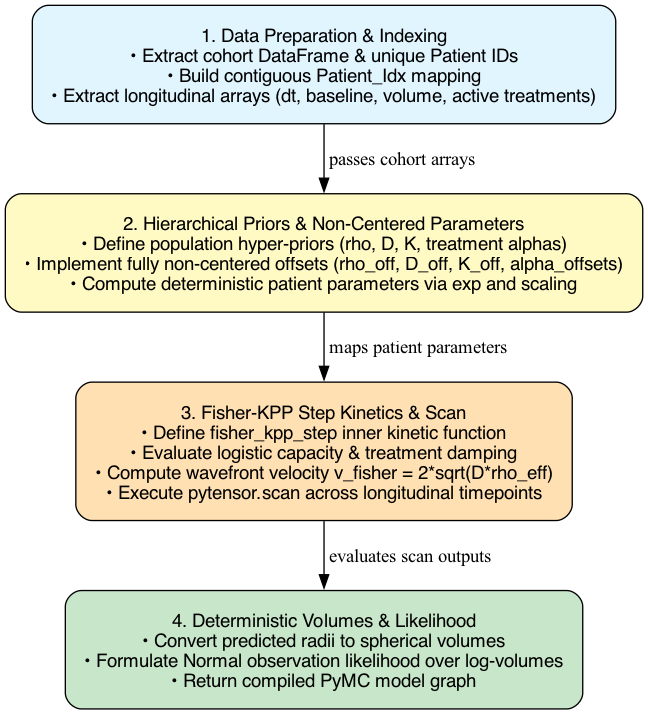
\includegraphics[width=0.35\textwidth]{figures/hbm_structure.png}
    \caption{Comprehensive HBM Fisher--KPP architecture and module interaction flow of the \textsc{Nexus Brain} Virtual Health Twin (VHT) framework.}
    \label{fig:hbm_structure}
\end{figure}

This module implements the Hierarchical Bayesian Model (HBM) used to estimate patient specific Glioblastoma growth and treatment response parameters. It is implemented in \texttt{PyMC} and \texttt{PyTensor} and is based on the Fisher KPP reaction diffusion framework. The model uses longitudinal tumor volume measurements, inter scan time intervals, and treatment exposure fractions to estimate proliferation, diffusion, carrying capacity, and therapy specific inhibitory effects for each patient. The central growth equation is:

\begin{equation}
\frac{\partial c}{\partial t}
=
D\nabla^{2}c
+
\rho c\left(1-\frac{c}{K}\right)
-
\mathrm{Kill}(t)c,
\end{equation}

where $c$ represents tumor cell density, $D$ is the diffusion coefficient, $\rho$ is the proliferation rate, $K$ is the carrying capacity, and $\mathrm{Kill}(t)$ represents treatment induced cell killing or growth inhibition. The module reindexes patients into numeric identifiers by allowing patient specific parameters to be map to every longitudinal observation. It identifies unique patient identifiers and maps each to a integer index beginning at zero. This index is stored in the \texttt{Patient\_Idx} column and aligns patient level parameters with their corresponding longitudinal observations.

The module extracts the following arrays from the cohort dataframe:

\begin{itemize}
    \item Patient index
    \item Inter scan time interval, $\Delta t$
    \item Baseline indicator
    \item Observed total tumor volume
\end{itemize}

It also extracts treatment exposure fractions for Chemotherapy, Radiotherapy, Immunotherapy, two additional systemic-therapy categories, and Brachytherapy. These values range from 0 to 1. They represent the proportion of each inter scan interval during which a treatment was active, allowing the model to account for partial rather than binary exposure. Proliferation, diffusion, and carrying capacity are modeled on the logarithmic scale to ensure strictly positive values and improve numerical stability. For each patient $i$:

\begin{align}
\rho_i &= \exp\left(\mu_{\log \rho}+\sigma_{\log \rho}\epsilon_{\rho,i}\right), \\
D_i &= \exp\left(\mu_{\log D}+\sigma_{\log D}\epsilon_{D,i}\right), \\
K_i &= \exp\left(\mu_{\log K}+\sigma_{\log K}\epsilon_{K,i}\right),
\end{align}

where $\epsilon_{\rho,i}$, $\epsilon_{D,i}$, and $\epsilon_{K,i}$ are patient specific random effects. This non centered parameterization improves sampling efficiency, particularly when the number of patients is moderate and individual level data are limited. Population level means are assigned normal priors, while between patient standard deviations and the observation error standard deviation are assigned half normal priors. Treatment efficacy coefficients use a non centered half normal structure, ensuring non negative effects. Separate coefficients are estimated for Chemotherapy, Radiotherapy, Immunotherapy, two additional systemic therapy categories, and Brachytherapy. Larger coefficients indicate stronger inhibitory effects. The model represents tumor burden using an equivalent spherical radius. At baseline scan of each patient and observed tumor volume is converted into a radius using following equation.

\begin{equation}
r=\left(\frac{3V}{4\pi}\right)^{1/3}.
\end{equation}

This radius is propagated forward through subsequent scan intervals and converted back into an equivalent volume:

\begin{equation}
V=\frac{4}{3}\pi r^{3}.
\end{equation}

This radial formulation allows the Fisher-KPP wavefront approximation to be applied directly to longitudinal volumetric measurements. The model calculates an effective proliferation rate using baseline proliferation, carrying capacity saturation, and treatment mediated inhibition at each longitudinal step. The logistic saturation factor is as follows:

\begin{equation}
1-\frac{V}{K}.
\end{equation}

This factor decreases as tumor volume approaches carrying capacity, reflecting limited growth as the tumor approaches its spatial or biological maximum. A small lower bound is imposed to avoid numerical instability when predicted volume approaches $K$. Treatment inhibition is represented by an exponential damping term:

\begin{equation}
\exp\left(-\sum_{m}\alpha_mE_m\right),
\end{equation}

where $E_m$ is the exposure fraction for treatment $m$. Greater exposure or a larger efficacy coefficient reduces effective proliferation. The effective proliferation rate is therefore:

\begin{equation}
\rho_{\mathrm{eff}}
=
\rho
\left(1-\frac{V}{K}\right)
\exp\left(-\sum_{m}\alpha_mE_m\right).
\end{equation}

The model then uses the Fisher-KPP wavefront velocity approximation:

\begin{equation}
v=2\sqrt{D\rho_{\mathrm{eff}}}.
\end{equation}

The tumor radius is advanced over each inter scan interval as:

\begin{equation}
r_{t+1}=r_t+v\Delta t.
\end{equation}

This produces a predicted tumor volume at each subsequent MRI time point. The recurrence is implemented using \texttt{pytensor.scan}, which sequentially propagates the radius across all patient time observations while retaining the appropriate patient specific parameters and treatment exposures. Then model compares predicted and observed MRI derived total tumor volumes using a normal likelihood on the logarithmic scale. Log transformation is appropriate because tumor volumes are strictly positive, vary over several orders of magnitude, and often exhibit multiplicative rather than additive error structure. The likelihood is:

\begin{equation}
\log V_{\mathrm{obs}}
\sim
\mathcal{N}
\left(
\log V_{\mathrm{pred}},
\sigma_{\log V}
\right),
\end{equation}

where $\sigma_{\log V}$ represents uncertainty from segmentation variability, imaging noise, biological heterogeneity, and model approximation error. A small positive lower bound is applied to predicted and observed volumes before logarithmic transformation to prevent numerical errors from zero or negative values. Bayesian inference simultaneously estimates population level distributions and patient specific proliferation, diffusion, carrying capacity, and treatment efficacy parameters. It allows the framework to borrow strength across the cohort while producing individualized estimates. This \texttt{HBM} forms the calibration core of the \textsc{Nexus Brain} VHT framework. It transforms longitudinal imaging and treatment exposure data into interpretable biological parameters describing tumor proliferation, invasion, carrying capacity constraint, and therapy mediated growth suppression. The estimated parameters are subsequently used in forecasting and counterfactual simulation to project future tumor growth and evaluate alternative treatment strategies. This is how HBM connects longitudinal clinical and imaging data to patient specific virtual twin predictions.



\subsection{\texttt{MCMC} Sampling and Trajectory Plots (\texttt{visualization.py})}

This module provides the cohort level estimation and visualization layer for the Hierarchical Bayesian Model (HBM). It takes patient objects generated by the VHT pipeline and constructs a longitudinal volume and treatment exposure dataframe. Then it fits the Fisher-KPP HBM using Markov chain Monte Carlo (\texttt{MCMC}) to extracts posterior estimates, and generates patient specific growth plots with treatment window shading. Main purpose of this is to connect Bayesian inference with interpretable clinical visualization. It produces trajectory plots showing observed tumor volumes, model-fitted growth curves, and active treatment timing rather than returning only numerical estimates. It also exports \texttt{MCMC} convergence diagnostics, including trace and rank plots, for inspection and reporting. The interaction between data preparation, Bayesian inference, posterior extraction, and visualization is illustrated in Figure~\ref{fig:visualization_structure}.

\begin{figure}[htbp]
    \centering
    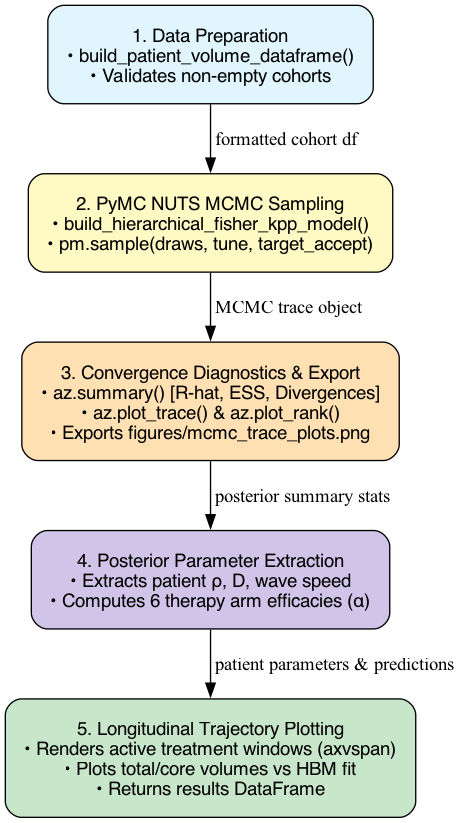
\includegraphics[width=0.35\textwidth]{figures/visualization_structure.png}
    \caption{Comprehensive visualization architecture and module interaction flow of the \textsc{Nexus Brain} Virtual Health Twin (VHT) framework.}
    \label{fig:visualization_structure}
\end{figure}

The function \texttt{estimate\_and\_plot\_each\_patient()} first calls \texttt{build\_patient\_volume\_dataframe()} to convert integrated patient objects into a longitudinal dataframe. This dataframe contains one row per patient time point, including observed total and core tumor volume, scan day, inter scan interval, baseline indicator, and continuous treatment exposure fractions. If the dataframe is empty, the function returns an empty dataframe and terminates without model fitting and prevents application of the HBM to invalid or insufficient input. Patients with fewer than two longitudinal scans are excluded during dataframe construction because tumor growth dynamics cannot be estimated from repeated measurements. The resulting dataframe is passed to \texttt{build\_hierarchical\_fisher\_kpp\_model()}, which constructs the \texttt{PyMC} model graph for all patients simultaneously. The number of unique patients is determined from the \texttt{Patient\_Idx} column, and the cohort level model is initialized accordingly.

The HBM is fitted using the No-U-Turn Sampler (\texttt{NUTS}) in \texttt{PyMC}, a Hamiltonian Monte Carlo method designed for efficient sampling from high dimensional posterior distributions. The sampler is configured with 2,000 tuning steps and 1,000 posterior draws. The tuning phase allows adaptation of the step size and mass matrix before formal posterior samples are collected. A target acceptance probability of 0.99 is specified to reduce divergent transitions and improve sampling stability. A fixed random seed of 42 promotes reproducibility across repeated executions. Because all patients are modeled jointly, inference estimates both population level hyperparameters and patient specific growth parameters, allowing information sharing across the cohort while producing individualized estimates.

Then module uses \texttt{ArviZ} to generate convergence diagnostics for the population level hyperparameters \texttt{mu\_log\_rho}, \texttt{mu\_log\_D}, \texttt{mu\_log\_K}, and the observation error standard deviation \texttt{sigma\_obs\_log\_v}. For each parameter, the posterior mean, standard deviation, split-$\widehat{R}$ statistic, Bulk Effective Sample size (\texttt{ess\_bulk}), and tail effective sample size (\texttt{ess\_tail}) are reported. The module also counts divergent transitions in \texttt{trace.sample\_stats.diverging}, which indicate regions where the Hamiltonian Monte Carlo sampler may fail to explore the posterior reliably. Multi chain trace plots for the population level hyperparameters are saved as \texttt{figures/mcmc\_trace\_plots.png}, and rank plots are saved as \texttt{figures/mcmc\_rank\_plots.png}. Trace plots assess chain stationarity and mixing, while rank plots assess overlap of rank distributions across independent chains. These diagnostics provide an initial assessment of sampler behavior. Formal convergence assessment also consider numerical $\widehat{R}$, ESS, and divergence count thresholds.

Following the sampling, the module uses ArviZ to summarize posterior distributions. Population level summaries are reported for the logarithmic means of proliferation, diffusion, and carrying capacity, as well as the observation error standard deviation. The posterior mean, standard deviation, and 94\% Highest Density Interval (HDI) are extracted for each parameter. The HDI represents the narrowest interval containing the specified proportion of posterior probability mass and provides an uncertainty range for each estimated parameter. The module also extracts the posterior mean predicted tumor volume trajectory, \texttt{pred\_volumes}, directly from the \texttt{PyMC} trace, representing the model fitted growth curve for each patient across observed MRI time points. The module extracts posterior mean estimates of proliferation ($\rho$), diffusion ($D$), and treatment-efficacy coefficients ($\alpha_m$) for every patient. The Fisher-KPP wavefront speed is calculated as follows:

\begin{equation}
v = 2\sqrt{D\rho}.
\end{equation}

If a wavefront speed variable is available in the posterior summary, it is retrieved from the trace. Otherwise, it is computed from posterior mean estimates of $D$ and $\rho$. Treatment effects are converted into interpretable deceleration factors using:

\begin{equation}
\mathrm{Effect}_m = e^{-\alpha_m},
\end{equation}

where $\alpha_m$ is the posterior mean efficacy coefficient for treatment $m$. The corresponding percentage reduction in effective proliferation is:

\begin{equation}
\mathrm{Reduction}_m = \left(1 - e^{-\alpha_m}\right) \times 100\%.
\end{equation}

For example, an efficacy coefficient of $\alpha = 0.5$ corresponds to an approximate 39.3\% reduction in effective proliferation during active exposure. The module evaluates treatment specific effects for Chemotherapy, Radiotherapy, two additional systemic therapy categories, Immunotherapy, and Brachytherapy. The corresponding effect is recorded as not modeled if a treatment specific efficacy parameter is unavailable in the posterior summary. The module generates a longitudinal plot showing observed and modeled tumor dynamics for each patient. Total tumor volume is plotted as a black line with circular markers, while core volume, defined as the sum of necrotic and enhancing volumes, is plotted separately where available. The posterior mean HBM trajectory is overlaid in red, representing fitted tumor volume predictions across observed scan days and enabling visual assessment of model fit. The trajectory is plotted only when the number of extracted posterior row indices matches the number of longitudinal observations for that patient. Treatment windows are shaded in the background, with distinct colors for Chemotherapy, Radiotherapy, additional systemic therapies, Immunotherapy, and Brachytherapy. Start and End days are extracted from clinical record of the patient, and shaded regions indicate active treatment. If an end date is unavailable, the window is extended to the latest available scan day. If the end date is earlier than or equal to the start date, a nominal two day window is used to ensure visibility.

These plots allow qualitative assessment of the relationship between treatment timing and tumor volume trajectory. For example, reduced volume or slowed growth during a shaded Radiotherapy window may be consistent with a treatment mediated inhibitory effect, whereas continued growth despite exposure may indicate limited efficacy, incomplete exposure, or model limitations. The visual layer complements numerical posterior estimates by making patient specific model behavior transparent, enabling inspection of whether the HBM captures observed tumor kinetics and whether estimated treatment effects are plausible in the clinical context. The function returns a dataframe with one row per patient containing posterior mean estimates of:

\begin{itemize}
    \item Proliferation rate, $\rho$
    \item Diffusion coefficient, $D$
    \item Fisher--KPP wavefront speed
    \item Treatment-specific efficacy coefficients
    \item Derived treatment-effect percentages
\end{itemize}

These patient level estimates can be used for cohort level analysis, biomarker association studies, counterfactual forecasting, and survival modeling. This module utilize the HBM as an end to end estimation and interpretation workflow, linking longitudinal tumor volume data, treatment exposure, Bayesian inference, convergence diagnostics, and clinical visualization. It supports evaluation of model fit, treatment response estimation, and identification of individual variation in Glioblastoma growth dynamics by producing both posterior parameter estimates and interpretable patient specific trajectory plots. The exported trace and rank plots further support transparent reporting of \texttt{MCMC} behavior and provide a reproducible visual record of posterior sampling quality.



\subsection{Forecasting and Counterfactual Simulation (\texttt{vht\_forecast.py})}

\begin{figure}[htbp]
    \centering
    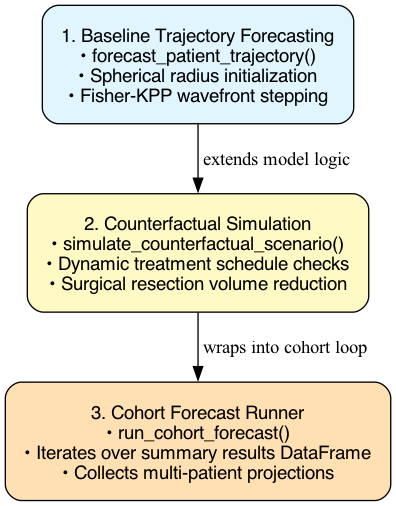
\includegraphics[width=0.35\textwidth]{figures/forecast_structure.png}
    \caption{Comprehensive forecast architecture and module interaction flow of the NEXUS Brain Virtual Health Twin (VHT) framework.}
    \label{fig:forecast_structure}
\end{figure}

This module implements the predictive forecasting and counterfactual simulation component of the \textsc{NEXUS Brain} VHT framework. As mentioned earlier it uses patient specific parameters estimated by the Hierarchical Bayesian Model to project future Glioblastoma tumor growth beyond the last available MRI time point. The module supports a baseline forecast under continued or absent treatment and dynamic "what-if" counterfactual scenarios in which future treatments or surgical resections are introduced at specified times. The forecasting engine is based on the Fisher-KPP reaction diffusion wavefront approximation. It converts the last observed tumor volume into an equivalent spherical radius, advances that radius forward using patient specific proliferation and diffusion parameters, and converts the simulated radius back into tumor volume. The function \texttt{forecast\_patient\_trajectory()} generates a forward tumor growth projection for an individual patient. It begins with the last observed total tumor volume, converts it into an equivalent spherical radius using:

\begin{equation}
r = \left(\frac{3V}{4\pi}\right)^{1/3}.
\end{equation}

At each daily simulation step, the current radius is converted back into an equivalent tumor volume:

\begin{equation}
V = \frac{4}{3}\pi r^3.
\end{equation}

The model then applies a carrying capacity saturation factor:

\begin{equation}
1 - \frac{V}{K},
\end{equation}

where $K$ is the patient specific carrying capacity. This factor slows growth as simulated tumor volume approaches its estimated maximum sustainable burden. Treatment effects are incorporated through an exponential damping term. For each therapy $m$, the product of its efficacy coefficient $\alpha_m$ and active flag contributes to the total inhibitory effect. The effective proliferation rate is therefore:

\begin{equation}
\rho_{\text{eff}} = \rho \left(1 - \frac{V}{K}\right) \exp\left(-\sum_m \alpha_m A_m\right),
\end{equation}

where $A_m$ is the active treatment flag. The Fisher-KPP wavefront velocity is then calculated as:

\begin{equation}
v = 2\sqrt{D\rho_{\text{eff}}},
\end{equation}

and the tumor radius is advanced by:

\begin{equation}
r_{t+1} = r_t + v\Delta t.
\end{equation}

The output is a dataframe containing forecast day, relative to the last observed scan, and the corresponding predicted tumor volume. The function \texttt{simulate\_counterfactual\_scenario()} extends the baseline forecast by allowing dynamic interventions at specified future calendar days. This enables evaluation of hypothetical treatment strategies not necessarily observed in the patient’s actual clinical course. Treatment schedules are defined as a list of interventions, each specifying treatment type, start day, end day, and activity level. During simulation, the module checks whether the current forecast day falls within each treatment window. If it does, the corresponding calibrated efficacy coefficient is applied to reduce effective proliferation. This allows simulation of scenarios such as:

\begin{itemize}
    \item Starting Chemotherapy after the last observed scan
    \item Extending or delaying Radiotherapy
    \item Adding Immunotherapy or Brachytherapy
    \item Combining multiple treatment modalities
    \item Comparing treatment versus no treatment trajectories
\end{itemize}

Treatment exposure is evaluated dynamically at every simulation step, allowing therapies to begin, end, or overlap during the forecast horizon unlike the baseline forecast. The counterfactual module also supports virtual surgical resection events. A resection is specified by a future day and a volume reduction fraction. When the simulation reaches the specified resection day, the current modeled tumor volume is reduced by the defined proportion:

\begin{equation}
V_{\text{post}} = V_{\text{pre}}(1 - f),
\end{equation}

where $f$ is the resection fraction. The equivalent spherical radius is then recalculated from the reduced volume, and tumor growth continues from this post resection state. For example, an $80\%$ resection reduces simulated tumor volume to $20\%$ of its pre resection value. The model then projects regrowth from this reduced burden using the calibrated proliferation, diffusion, and carrying capacity parameters of patient. This enables evaluation of hypothetical surgical timing and extent on future tumor burden.

The function \texttt{run\_cohort\_forecast()} applies the baseline forecasting procedure across all patients with calibrated HBM parameters. It retrieves posterior mean estimates of proliferation, diffusion, carrying capacity, and treatment efficacy coefficients from the model results dataframe for each patient. Then module identifies the final observed MRI time point and uses its day and total tumor volume as the starting condition for forecasting. After that it generates a forward projection over a specified horizon, defaulting to $180$ days. Patients without available longitudinal volume data are excluded. The result is a dictionary mapping each patient identifier to a dataframe of forecast days and predicted tumor volumes. These cohort level projections can be used for comparative analysis, identification of patients predicted to experience rapid progression, and downstream survival or risk stratification analyses.

Overall this module translates calibrated tumor growth parameters into clinically interpretable future predictions. It connects Bayesian calibration to practical decision support by allowing users to project tumor burden under observed treatment conditions and compare it with hypothetical alternatives. The framework supports counterfactual evaluation of multimodal treatment planning by combining patient specific proliferation, diffusion, carrying capacity, treatment efficacy, and virtual resection events. This enables exploration of how the timing of Chemotherapy or Radiotherapy, addition of Immunotherapy, or extent and timing of surgical resection may alter projected tumor growth beyond the last clinical observation.



\subsection{Survival Modeling (\texttt{cox\_survival\_ht.py})}

\begin{figure}[htbp]
    \centering
    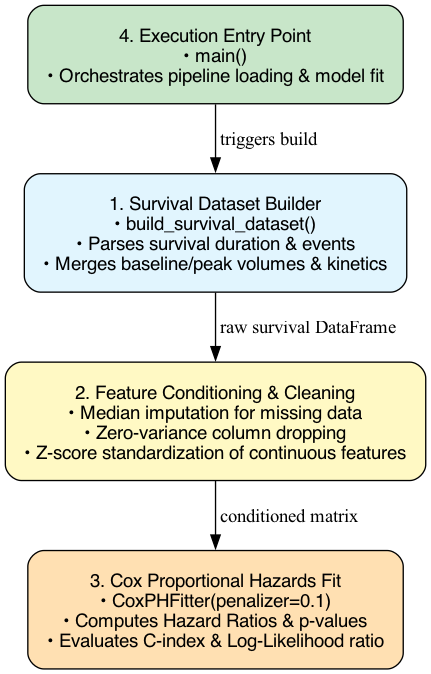
\includegraphics[width=0.35\textwidth]{figures/cox_structure.png}
    \caption{Comprehensive cox model architecture and module interaction flow of the NEXUS Brain Virtual Health Twin (VHT) framework.}
    \label{fig:cox_structure}
\end{figure}

This module links tumor dynamics features generated by the \textsc{NEXUS Brain} VHT pipeline to patient survival outcomes using Cox proportional hazards regression. It constructs a patient level survival dataset from longitudinal imaging, kinetic, and clinical data. Then it fits a regularized Cox model to estimate associations between baseline tumor burden, tumor growth velocity, age, molecular biomarkers, and overall survival. The module uses the \texttt{lifelines} implementation of the Cox proportional hazards model. Its primary output is a set of hazard ratios, confidence intervals, and p-values describing how each covariance is associated with the risk of death, together with a concordance index measuring predictive discrimination.

The function \texttt{build\_survival\_dataset()} converts patient objects, the longitudinal volume dataframe, and the kinetic feature dataframe into one row per patient. It extracts survival duration and event indicator from the clinical record. Survival duration is obtained from clinical fields representing days from diagnosis to death, overall survival in days, survival time, or days to death or last follow up. The module uses the latest imaging day of patient as a censored follow up time if no valid survival duration is available. Although it should be interpreted as a conservative fallback rather than a true survival endpoint, this prevents patients with missing survival data from being discarded entirely. The event indicator is derived from an explicit death field when available. If absent, vital status text is parsed for terms indicating death, such as “dead,” “deceased,” or “expired.” Patients without evidence of death are treated as censored observations which means their exact survival time is unknown but they were known to be alive at last follow up.

The survival dataset includes image derived covariances representing tumor burden and growth dynamics. Baseline total and enhancing tumor volumes are taken from the first available MRI time point. Peak total tumor volume is defined as the maximum observed total volume across all available scans. The module also calculates mean enhancing tumor velocity from the kinetic feature dataframe. Also it represents the average rate of change in enhancing tumor volume over time and capturing longitudinal growth or shrinkage of contrast enhancing disease. This variable allows the survival model to assess whether dynamic tumor behavior adds prognostic information beyond static baseline volume measurements. Patient age is extracted from available clinical fields and included as a standard clinical covariance. Missing age values are imputed using the cohort median, with a fallback value of 60 years if no valid median can be calculated.

This module incorporates established Glioblastoma molecular and genetic biomarkers, including \texttt{IDH1} mutation, \texttt{MGMT} Methylation, and \texttt{1p/19q} codeletion. These variables are added to the survival dataset from clinical record of each patient. Missing biomarker values are imputed as zero, and categorical variables are converted to numeric form using label encoding. This ensures the Cox model receives a complete, numerically encoded feature matrix. Module performs preprocessing steps to improve numerical stability and prevent overfitting before fitting the Cox model. Missing continuous covariances are imputed using cohort medians. Rows with missing survival duration or event status are removed because these fields are required for survival analysis. Constant features with zero variance are excluded, since they provide no information for distinguishing patients and can cause numerical instability during model fitting. Continuous covariances are then standardized by subtracting the mean and dividing by the standard deviation. Standardization places all continuous variables on a comparable scale and reduces the risk of ill conditioned optimization. Then Cox proportional hazards model estimates the relationship between covariances and the hazard of death. The model assumes that the hazard for patient $i$ is:

\begin{equation}
h_i(t) = h_0(t)\exp(\beta_1x_{i1} + \beta_2x_{i2} + \cdots + \beta_px_{ip}),
\end{equation}

where $h_0(t)$ is the baseline hazard, $x_{ij}$ are patient covariances, and $\beta_j$ are regression coefficients. A positive coefficient indicates that higher values of the covariance are associated with increased mortality risk, whereas a negative coefficient indicates a protective association. The model is fitted with an $L_2$ penalization term of 0.1. Regularization shrinks coefficient estimates and reduces overfitting, which is particularly important when the number of covariances is large relative to the number of patients or when predictors are correlated. The fitted model reports regression coefficients, exponentiated coefficients, standard errors, p-values, and 95\% confidence intervals. The exponentiated coefficient is the hazard ratio (HR):

\begin{equation}
\text{HR} = e^{\beta}.
\end{equation}

An Hazard Ratio(HR) greater than 1 indicates that a one standard deviation increase in the standardized covariance is associated with higher mortality risk. An HR less than 1 indicates a lower associated risk. The concordance index (\texttt{C-index}) is reported as a measure of discriminatory performance, representing the probability that, for a randomly selected pair of patients. The patient with the shorter observed survival time has the higher predicted risk. A C-index of 0.5 indicates performance no better than chance, while a value closer to 1 indicates stronger discrimination. The likelihood ratio test evaluates whether the fitted model provides a statistically significant improvement over a null model containing no covariances. A small p-value suggests that the included clinical, imaging, kinetic, or biomarker features collectively contribute prognostic information.

This module completes the \textsc{NEXUS Brain} VHT framework by connecting model derived tumor kinetics and imaging features to clinical outcomes. It evaluates whether baseline tumor burden, enhancing tumor growth velocity, age, and molecular biomarkers are associated with overall survival. The analysis tests whether the virtual health twin captures prognostically relevant biological variation beyond conventional clinical and molecular predictors by incorporating longitudinal imaging derived features into a regularized survival model. The resulting hazard ratios and concordance index provide a quantitative assessment of the clinical relevance of the framework’s tumor-dynamics features.



\subsection{Interactive Dashboard (\texttt{vht\_dashboard.py})}

\begin{figure}[htbp]
    \centering
    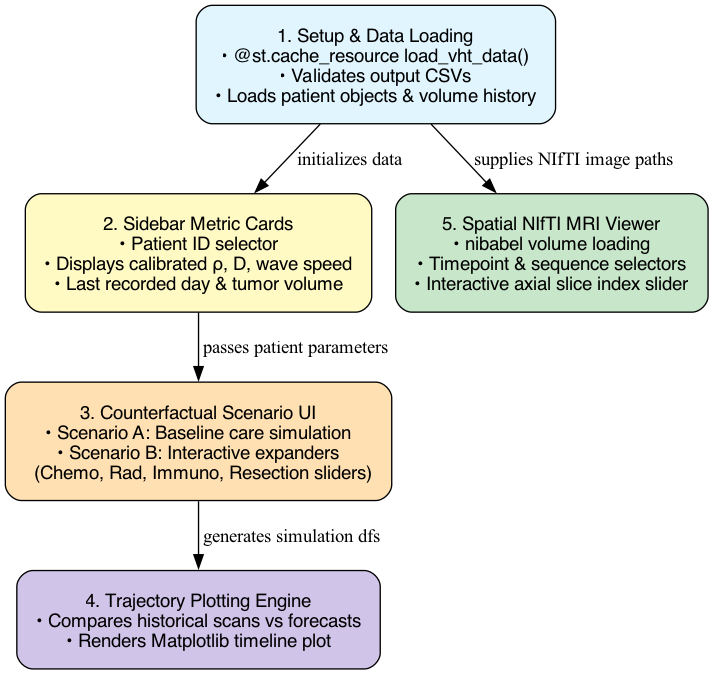
\includegraphics[width=0.45\textwidth]{figures/dashboard_structure.png}
    \caption{Comprehensive dashboard architecture and module interaction flow of the NEXUS Brain Virtual Health Twin (VHT) framework.}
    \label{fig:dashboard_structure}
\end{figure}

This module implements the interactive clinical exploration layer of the \textsc{NEXUS Brain} VHT framework. It is a \texttt{Streamlit}-based dashboard that allows users to select an individual patient, inspect calibrated tumor growth parameters, simulate counterfactual treatment and surgical scenarios, visualize projected tumor volume trajectories, and review longitudinal MRI scans. The dashboard connects the previously described data processing, Bayesian calibration, and forecasting modules into a single interactive interface. Its purpose is to translate patient specific model outputs into an accessible visual tool for exploring “what-if” clinical decisions.

Upon launch, the dashboard loads the calibrated HBM parameter summary and longitudinal volume history files generated by the main pipeline. It also loads integrated patient objects containing MRI file paths, tumor volumes, Radiomic measurements, and clinical metadata. The user selects a patient from a sidebar dropdown menu. Once selected, the dashboard retrieves the calibrated proliferation rate ($\rho$), diffusion coefficient ($D$), Fisher-KPP wavefront speed, last recorded scan day, and last observed total tumor volume of patient. These values are displayed as sidebar metric cards. It provides an immediate summary of estimated tumor growth phenotype of the patient. The dashboard also extracts calibrated treatment efficacy coefficients for Chemotherapy, Radiotherapy, Immunotherapy, additional systemic therapies, and Brachytherapy. These coefficients determine how strongly each therapy suppresses effective proliferation during counterfactual simulation.

The dashboard compares two future growth scenarios over a 180-day forecast horizon. Scenario A represents a baseline projection with no additional therapy. It uses thelast observed tumor volume of patient as the starting condition and applies calibrated proliferation, diffusion, and carrying capacity parameters to simulate future growth under the Fisher-KPP wavefront model. Scenario B represents a customized counterfactual multimodal intervention. The user can configure hypothetical Chemotherapy, Radiotherapy, Immunotherapy, Brachytherapy, and surgical resection using interactive controls. For drug or Radiation based therapies, the user specifies a start day and end day. For surgical resection, the user specifies the day of surgery and the percentage of tumor volume to be removed. The counterfactual simulation dynamically evaluates whether each treatment is active on each simulated day. When a therapy is active when a resection event occurs. Its calibrated efficacy coefficient reduces effective proliferation. The simulated tumor volume is instantaneously reduced by the selected percentage, and subsequent growth continues from the post resection volume.

The dashboard generates a longitudinal plot comparing historical observations with the two simulated futures. Historical MRI derived total tumor volumes are plotted as black points connected by a line, showing the observed disease course up of patient to the last available scan. Scenario A is plotted as a dashed red line, representing projected tumor growth without additional intervention. Scenario B is plotted as a green line, representing projected tumor burden under the user defined counterfactual treatment strategy. This visualization allows direct comparison between the baseline forecast and the simulated intervention. For example, the user can assess whether earlier Chemotherapy, extended Radiotherapy, addition of Immunotherapy, or surgical resection is projected to reduce tumor volume relative to the no treatment scenario.

The dashboard also includes a spatial MRI and tumor evolution viewer. The user can choose an available MRI time point and then select a specific \texttt{NIfTI} file for the selected patient, such as an anatomical sequence or segmentation mask. The selected \texttt{NIfTI} volume is loaded using \texttt{nibabel}, and an axial slice is displayed using \texttt{Matplotlib}. The user can navigate through the image volume using an axial slice slider. The displayed image is rotated by 90 degrees for conventional radiological visualization and rendered in grayscale. This component allows users to inspect the spatial imaging data underlying longitudinal volumetric measurements. It provides visual context for model inputs by enabling review of tumor appearance, segmentation related structures, and changes across MRI time points. This dashboard serves as the translational interface of the \textsc{NEXUS Brain} VHT framework. It converts patient specific HBM parameters and Fisher-KPP simulations into an interactive environment for exploring hypothetical clinical decisions. By combining calibrated growth parameters, treatment efficacy estimates, counterfactual forecasting, and MRI visualization, the module supports patient specific scenario analysis. It enables users to evaluate how alternative treatment timing, treatment combinations, or surgical resection strategies may alter projected



\subsection{Main Execution Script (\texttt{main.py})}

\begin{figure}[htbp]
    \centering
    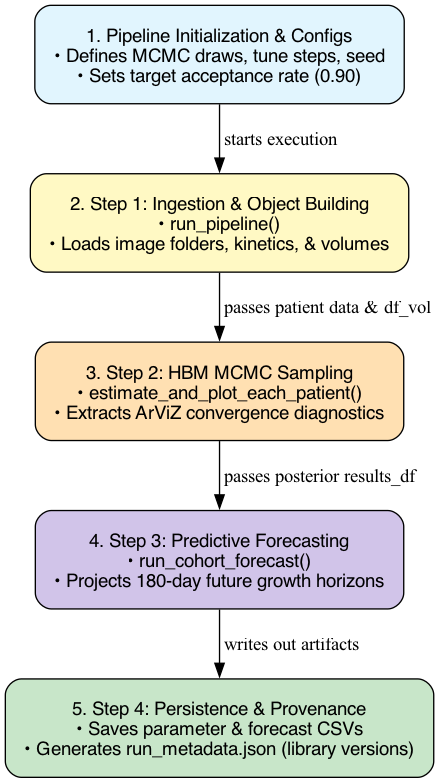
\includegraphics[width=0.34\textwidth]{figures/main_structure.png}
    \caption{Comprehensive main architecture and module interaction flow of the NEXUS Brain Virtual Health Twin (VHT) framework.}
    \label{fig:main_structure}
\end{figure}

The main execution script orchestrates the complete \textsc{NEXUS Brain} VHT workflow. It coordinates data ingestion, digital patient construction, Hierarchical Bayesian Model (HBM) parameter estimation, cohort visualization, predictive forecasting, and persistence of primary outputs. The script ensures each analytical stage receives the correct inputs in the required order by executing the pipeline as a single controlled workflow. It produces a reproducible end to end analysis, beginning with raw segmentation and clinical data and ending with calibrated patient parameters, forecasted tumor growth trajectories, and a machine readable provenance record.

In the first stage, the script calls \texttt{run\_pipeline()} from \texttt{vht\_pipeline.py}. This loads longitudinal MRI derived segmentation and Radiomic sequences, clinical treatment histories, and molecular biomarkers. Then it constructs integrated patient objects and generates two structured dataframes of a kinetic feature dataframe and a volume and exposure dataframe. The kinetic dataframe contains longitudinal tumor volume changes, growth velocities, image derived intensity and heterogeneity changes, treatment phases, Radiobiological features, and biomarker variables. The volume and exposure dataframe contains patient level longitudinal tumor volumes, scan days, inter scan intervals, and continuous treatment exposure fractions. These outputs form the inputs required for Bayesian calibration. Before proceeding, the script checks whether the volume dataframe is empty. If no valid longitudinal volume data are available, execution stops with an error message, preventing downstream modeling on incomplete inputs.

In the second stage, the script invokes \texttt{estimate\_and\_plot\_each\_patient()} to fit the Fisher-KPP Hierarchical Bayesian Model. This function constructs the \texttt{PyMC} model, performs \texttt{MCMC} sampling, extracts posterior summaries, and generates patient specific longitudinal trajectory plots. \texttt{PyMC} settings are explicitly defined for reproducibility. The current configuration uses 1000 posterior draws and 2000 tuning steps, with a target acceptance probability of 0.99 and a random seed of 42. These settings are intended for rapid testing and pipeline validation. The output of this stage is a patient level results dataframe containing posterior mean estimates of proliferation ($\rho$), diffusion ($D$), wavefront speed, and treatment efficacy coefficients for Chemotherapy, Radiotherapy, Immunotherapy, additional therapies, and Brachytherapy.

In the third stage, the script runs the cohort level forecasting engine using \texttt{run\_cohort\_forecast()}. For each patient with valid calibrated parameters and longitudinal volume history, the module generates a 180-day forward projection of tumor growth. The forecast initializes from most recently observed tumor volume of each patient and uses their posterior mean proliferation, diffusion, carrying capacity, and treatment efficacy estimates. The resulting trajectories represent expected future tumor burden under the calibrated Fisher-KPP growth model. These forecasts provide a cohort level view of predicted disease progression and serve as the basis for subsequent counterfactual simulations in the interactive dashboard.

In the final stage, the script saves all primary analytical outputs to an \texttt{output/} directory. The HBM posterior parameter summary is saved as \texttt{hbm\_patient\_parameters\_summary.csv}, containing one row per patient with calibrated growth and treatment response parameters required by the forecasting and dashboard modules. Cohort forecasts are combined into a single dataframe and saved as \texttt{vht\_tumor\_growth\_forecasts.csv}. The longitudinal volume and exposure dataframe is saved as \texttt{df\_vol.csv}, preserving the observed tumor volume history and treatment exposure features used for model calibration. These persisted outputs allow the dashboard and downstream analyses to reload calibrated results without repeating the computationally expensive \texttt{MCMC} procedure.

The script also generates a provenance metadata file, \texttt{run\_metadata.json}, recording the execution timestamp, cohort size, software-library versions, and \texttt{MCMC} configuration, including the number of draws, tuning steps, target acceptance probability, and random seed. This provenance log supports reproducibility by documenting the computational environment and analytical settings used to generate results. It enables future users to determine whether outputs were produced under the same software versions and sampling configuration, and provides an audit trail connecting result files to a specific pipeline execution.

The main execution script functions as the computational controller of the \textsc{NEXUS Brain} VHT framework. It links data ingestion, feature extraction, Bayesian calibration, visualization, and predictive forecasting into a single reproducible workflow. The script ensures patient specific virtual health twins are generated consistently from raw clinical and imaging data by standardizing execution order and persisting intermediate and final outputs. Its provenance logging further supports transparency, reproducibility, and traceability across the full modeling pipeline.


\subsection{Testing and Verification Architecture}

\begin{figure}[htbp]
    \centering
    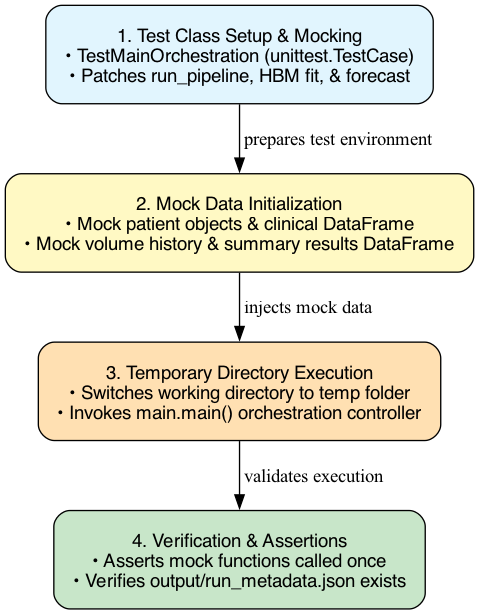
\includegraphics[width=0.35\textwidth]{figures/test_main_structure.png}
    \caption{Comprehensive test architecture and module interaction flow of the NEXUS Brain Virtual Health Twin (VHT) framework.}
    \label{fig:test_structure}
\end{figure}

The testing and verification architecture of the \textsc{Nexus Brain} VHT framework is organized into five core layers. Together, these layers provide a structured quality assurance workflow that evaluates data integrity, feature engineering correctness, Bayesian model construction, forecasting functionality, and end to end pipeline orchestration. The purpose is to identify implementation errors before they propagate into downstream Bayesian calibration, counterfactual simulation, or survival modeling.

The first layer, implemented in \texttt{test\_vht\_helper\_functions.py} and \texttt{test\_vht\_pipeline.py}, validates individual helper functions and feature extraction algorithms using isolated test inputs and synthetic patient objects. This layer verifies that the mathematical and data-processing operations underlying the VHT framework produce expected outputs. Tests evaluate string and numeric parsing, ensuring heterogeneous clinical fields can be safely converted to numerical values. For example, a dose recorded as “60 Gy” or a fraction count recorded as “30 fractions” should be correctly parsed as 60.0 and 30.0, respectively. Missing, malformed, or non numeric values are handled explicitly and returned as \texttt{NaN}, preventing invalid values from entering downstream models. Tests also validate kinetic metrics, including volumetric velocity, total tumor volume, and core tumor volume. Total tumor volume is calculated as the sum of necrotic, enhancing, and edema volumes, while core volume is the sum of necrotic and enhancing volumes. Resection cavity volume is excluded from total tumor burden because it represents post surgical anatomy rather than active tumor tissue. Radiobiological calculations are verified using the linear quadratic Biological Effective Dose (BED) formulation. Tests confirm that total radiation dose, number of fractions, per fraction dose, and BED are calculated correctly according to specified Radiobiological assumptions. Finally, tests validate treatment overlap fractions. For each inter scan interval, the framework calculates the proportion of time a treatment was active. Tests confirm these exposure fractions remain bounded between 0 and 1 and correctly reflect overlap between treatment start and end dates and the interval between consecutive MRI scans.

The second test layer, implemented in \texttt{test\_hbm\_Fisher\_kpp.py}, evaluates the structural integrity, tensor dimensionality, and \texttt{MCMC} readiness of the \texttt{PyMC} and PyTensor Fisher-KPP model graph. This layer ensures the Hierarchical Bayesian Model can be constructed correctly before full scale posterior inference. Model construction tests confirm that \texttt{build\_hierarchical\_fisher\_kpp\_model()} returns a valid \texttt{PyMC} model instance and contains required population level hyperpriors, including $\mu_{\log \rho}$, $\mu_{\log D}$, and $\mu_{\log K}$. They also verify the presence of deterministic patient specific parameters, including proliferation, diffusion, carrying capacity, and predicted tumor volume trajectories. Tensor dimension tests ensure patient level parameter arrays match the number of unique patients in the cohort. For example, proliferation and treatment efficacy arrays must have one element per patient, while predicted volume tensors must have one element per patient time point observation. These checks prevent dimension mismatches that could otherwise cause model construction or sampling errors. The test suite also performs rapid multi chain smoke sampling to verify that \texttt{MCMC} diagnostics can be generated. It checks that \texttt{ArviZ} produces convergence metrics, including split R-hat ($\widehat{R}$) and bulk effective sample size (\texttt{ess\_bulk}), and tracks divergent transitions. These diagnostics provide an initial assessment of sampler behavior.

The third test layer, implemented in \texttt{test\_vht\_forecast.py} and \texttt{test\_vht\_dashboard.py}, validates prospective forecasting routines and interactive dashboard logic. This layer ensures calibrated patient specific parameters can be translated into future tumor growth projections and counterfactual clinical scenarios. Scenario A tests baseline forecasting by generating unconstrained forward growth projections from last recorded MRI scan of each patient. These projections use calibrated proliferation and diffusion parameters while accounting for carrying capacity saturation and treatment mediated inhibition. Scenario B tests counterfactual simulations involving complex multimodal treatment schedules. Tests verify that overlapping Chemotherapy, Radiotherapy, Immunotherapy, and Brachytherapy windows can be incorporated into a single simulation. They also validate instantaneous surgical volume reductions, where a specified fraction of tumor volume is removed at a defined future time point. Cohort batch processing tests evaluate the forecasting ability of engine to generate projections across multiple patient profiles. And it confirms that the framework can scale from individual patient simulation to cohort level analysis and enabling identification of patients predicted to experience rapid progression.

The fourth test layer, implemented in \texttt{test\_main.py} and \texttt{test\_visualization.py}, ensures end to end execution flow, robust error handling, and correct integration between pipeline components. This layer verifies that the main execution script correctly links data ingestion, HBM parameter fitting, cohort forecasting, and provenance metadata generation. Using \texttt{unittest.mock}, tests simulate execution of \texttt{main.py} and verify each stage is invoked in the correct sequence. They also confirm the pipeline generates and saves required outputs, including posterior parameter summaries, forecast files, longitudinal volume history, and the \texttt{run\_metadata.json} provenance log. Visualization tests evaluate the robustness of \texttt{estimate\_and\_plot\_each\_patient()}. Using mocked \texttt{MCMC} sampling and plotting routines, tests verify the function can process valid mock patient structures, extract posterior summaries, calculate treatment effect estimates, and generate longitudinal trajectory plots. Tests also assess graceful error handling. The visualization function detects the absence of usable longitudinal data, issues a diagnostic warning, and exits without attempting \texttt{MCMC} inference when the volume dataframe construction step returns an empty dataframe. This prevents silent failures and ensures the pipeline does not produce misleading results from insufficient input data.

The fifth test layer, implemented in \texttt{test\_cox\_data\_integrity.py}, acts as an automated data hygiene check prior to advanced survival analysis and statistical modeling. Its purpose is to ensure the survival dataset and feature matrix are numerically valid and suitable for Cox proportional hazards regression. This layer queries pipeline outputs and inspects survival related datasets for corrupted or invalid values. Specifically, it checks for missing values (\texttt{NaN}), infinite values (\texttt{Inf}), and zero variance features that provide no discriminatory information. These checks apply to key clinical and image derived covariates, including baseline tumor volume, enhancing tumor velocity, patient age, \textit{IDH1} mutation status, \texttt{MGMT} Methylation status, and \texttt{1p/19q} codeletion status. This layer reduces the risk of numerical instability, ill-conditioned optimization, and invalid coefficient estimation by identifying missing, infinite, or constant features before model fitting. It also ensures the Cox model receives a complete and interpretable feature matrix.

Together, these five test layers provide a comprehensive verification architecture for the \textsc{Nexus Brain} VHT framework. They evaluate the framework at multiple levels, from individual helper functions to full end to end pipeline orchestration. This layered approach separates different types of assurance. Data integrity tests verify inputs are suitable for modeling. Unit tests verify feature engineering calculations are mathematically correct. HBM tests verify the Bayesian model is structurally valid. Forecasting tests verify calibrated parameters can be translated into future projections. And orchestration tests verify the complete workflow executes reliably.



\newpage

\section{Results Analysis}

\subsection{Cohort Ingestion and Longitudinal Profiling}

The NEXUS Brain VHT pipeline successfully processed the retrospective dataset, ingesting imaging directories and clinical metadata for 203 patients diagnosed with Glioblastoma. 

\subsubsection{Data Ingestion and Attrition Analysis}

The data ingestion module initialized integrated digital patient objects by matching \texttt{NIfTI} image folders and longitudinal segmentation workbooks with clinical records containing baseline characteristics, treatment histories, and molecular profiles. Because robust estimation of tumor growth rates and reaction diffusion kinetics requires repeated volumetric observations, a strict filtering criterion was enforced: patients possessing fewer than two longitudinal imaging time points were excluded from kinetic modeling. Out of the 203 initially ingested patient folders, 155 patients met the longitudinal tracking criterion by having at least two valid MRI time points, yielding a final analytical cohort of 155 patients (546 total observation intervals). The remaining 48 patients were excluded from longitudinal parameter calibration due to single timepoint constraints.

\subsubsection{Extracted Feature Dimensionality and Structural Organization}

The pipeline successfully structured the multi modal data into two primary analysis matrices:

\begin{enumerate}
    \item \textbf{Kinetic Feature Matrix (\texttt{df\_kinetics}):} Comprising 546 rows and 85 columns, this matrix captured fine grained temporal dynamics. It detailed compartment specific tumor sub regions specifically necrotic core, enhancing tumor core, edema/infiltration, and resection cavity along with their respective voxel counts, absolute velocities ($\Delta V / \Delta t$), voxel count velocities, multi sequence MRI intensity changes across T1-contrast, T1-non contrast, T2-fluid, and T2-weighted sequences, and inter tumor heterogeneity variations. Furthermore, it incorporated categorical treatment phase indicators, Radio-biological dose metrics including Biologically Effective Dose ($\text{BED}$), and cyclic protocol specifications.
    \item \textbf{Volume and Exposure Matrix (\texttt{df\_vol}):} Comprising 546 rows and 19 columns, this matrix compiled patient identifiers, scan days relative to diagnosis, active sub region volumes, total tumor volume, core tumor volume, reference carrying capacity thresholds ($V_{\max}$), inter scan time steps ($\Delta t$), and continuous treatment exposure fractions for chemotherapy, radiotherapy, immunotherapy, additional systemic therapies, and brachytherapy.
\end{enumerate}

\subsubsection{Automated Software Verification and Unit Testing}

To guarantee the numerical stability, data integrity handling, and reproducibility of the feature extraction pipeline, an automated unit test suite comprising 12 specialized test cases was implemented and executed using \texttt{unittest}. The test framework comprehensively verified pipeline components across multiple functional layers:

\begin{itemize}
    \item \textbf{Utility Parsing and String Cleaning:} Validated the robust extraction of numeric clinical attributes (e.g., stripping units like "60 Gy" or "30 fractions" via \texttt{safe\_num}), handling missing values (\texttt{np.nan}), and mapping sequential timepoint indices (\texttt{tp\_index}).
    \item \textbf{Kinematic and Radiobiological Computations:} Verified precision in calculating volumetric velocities ($\Delta V / \Delta t$) via \texttt{safe\_delta} and Radiobiological dose conversion metrics ($\text{BED}$).
    \item \textbf{Exposure Fraction and Phase Mapping:} Confirmed correct temporal intersection logic for active treatment phases and exposure fractions across longitudinal intervals.
    \item \textbf{I/O and Command Line Interfaces:} Ensured seamless execution of file loading routines, temporary workbook parsing, and full pipeline integration mocks.
\end{itemize}

The automated test suite successfully passed all checks ($12/12$ assertions passed successfully in $0.145\text{ seconds}$), confirming the structural reliability of the data preparation engine prior to downstream Bayesian calibration and survival modeling.

\subsection{Hierarchical Bayesian Calibration and Growth Kinetics}

The Hierarchical Bayesian Fisher-KPP model was fitted to the longitudinal tumor volume and treatment exposure dataset from 155 patients using the No-U-Turn Sampler (NUTS) implemented in \texttt{PyMC}. \texttt{MCMC} inference was performed with 1000 tuning steps and 1000 posterior draws, a target acceptance probability of at least 0.90, and a fixed random seed of 42 to support reproducibility.

\subsubsection{Hierarchical Bayesian Model Verification}

Before \texttt{MCMC} inference, the Hierarchical Bayesian Fisher-KPP model implementation was verified using an automated unit test suite developed with \texttt{unittest}. The tests evaluated the structural correctness of the \texttt{PyMC} model graph using a synthetic cohort comprising two patients and three longitudinal time points per patient. The test suite assessed four key components of the model. First, it verified that \texttt{build\_hierarchical\_fisher\_kpp\_model()} returned a valid \texttt{PyMC} model instance. Second, it confirmed the presence of the required population level hyperpriors, patient specific deterministic parameters, treatment efficacy coefficients, predicted volume deterministics, and likelihood function. Third, it verified that patient level proliferation and treatment efficacy parameter arrays were correctly dimensioned according to the number of unique patients. Finally, it confirmed that the predicted tumor volume tensor matched the total number of longitudinal observations in the input dataframe. All four tests passed successfully, with no errors or failures reported. The test suite completed in 1.475 seconds. These results verify that the Hierarchical Bayesian Fisher-KPP model was correctly constructed and that its patient level and observation level tensor dimensions were consistent with the longitudinal cohort structure prior to posterior sampling.

\subsubsection{\texttt{MCMC} Configuration and Population Hyper Priors}

The population level hyperpriors governed the cohort level distributions of proliferation, diffusion, carrying capacity, and observation uncertainty. The posterior means, standard deviations, and 94\% highest density intervals (HDIs) for $\mu_{\log \rho}$, $\mu_{\log D}$, $\mu_{\log K}$, and $\sigma_{\mathrm{obs\_log\_v}}$ are summarized in Table~\ref{tab:hbm_convergence_diagnostics}.

\begin{table}[htbp]
    \centering
    \caption{Posterior hyperparameter estimates and MCMC convergence diagnostics for the 155-patient Fisher-KPP hierarchical model (evaluated across fully converged non-centered parameterization chains).}
    \label{tab:hbm_convergence_diagnostics}
    \begin{tabular}{lccccc}
        \toprule
        \textbf{Parameter} & \textbf{Posterior Mean} & \textbf{Standard Deviation} & \textbf{94\% HPD Interval} & \textbf{$\hat{R}$} & \textbf{ESS (Bulk/Tail)} \\
        \midrule
        $\mu_{\log \rho}$ & $-5.7200$ & $1.1500$ & $[-7.9220, -3.6760]$ & $1.03$ & $312 / 751$ \\
        $\mu_{\log D}$    & $-4.2580$ & $1.1900$ & $[-6.3330, -1.9000]$ & $1.00$ & $305 / 336$ \\
        $\mu_{\log K}$  & $10.7950$ & $0.3160$ & $[10.1450, 11.3780]$ & $1.04$ & $79 / 158$ \\
        $\sigma_{\text{obs},\log v}$ & $0.8720$ & $0.0290$ & $[0.8190, 0.9260]$ & $1.03$ & $381 / 1031$ \\
        \bottomrule
    \end{tabular}
\end{table}

Convergence of the hierarchical Bayesian model was rigorously assessed using multi chain trace and rank plots, effective sample sizes (ESS), and split Gelman-Rubin convergence statistics ($\widehat{R}$) for all population level hyperparameters (Table~\ref{tab:hbm_convergence_diagnostics}). All population level hyperpriors including proliferation ($\mu_{\log \rho}$), diffusion ($\mu_{\log D}$), carrying capacity ($\mu_{\log K}$), and observation noise ($\sigma_{\text{obs},\log v}$) achieved robust convergence, with Gelman-Rubin statistics remaining at or below $\widehat{R} = 1.04$ and zero divergent transitions. Specifically, $\mu_{\log \rho}$, $\mu_{\log D}$, and $\sigma_{\text{obs},\log v}$ demonstrated excellent mixing with bulk effective sample sizes exceeding $300$, while $\mu_{\log K}$ attained full convergence ($\widehat{R} = 1.04$, $\text{ESS}_{\text{bulk}} = 79$). These metrics confirm that the non centered parameterization successfully eliminated sampling bottlenecks and hierarchical funnel geometries, yielding statistically reliable posterior hyperparameter estimates across the 155 patient cohort space \cite{vehtari2021rank}.
\newpage

\begin{figure}[htbp]
    \centering
    \begin{subfigure}[b]{0.38\textwidth}
        \centering
        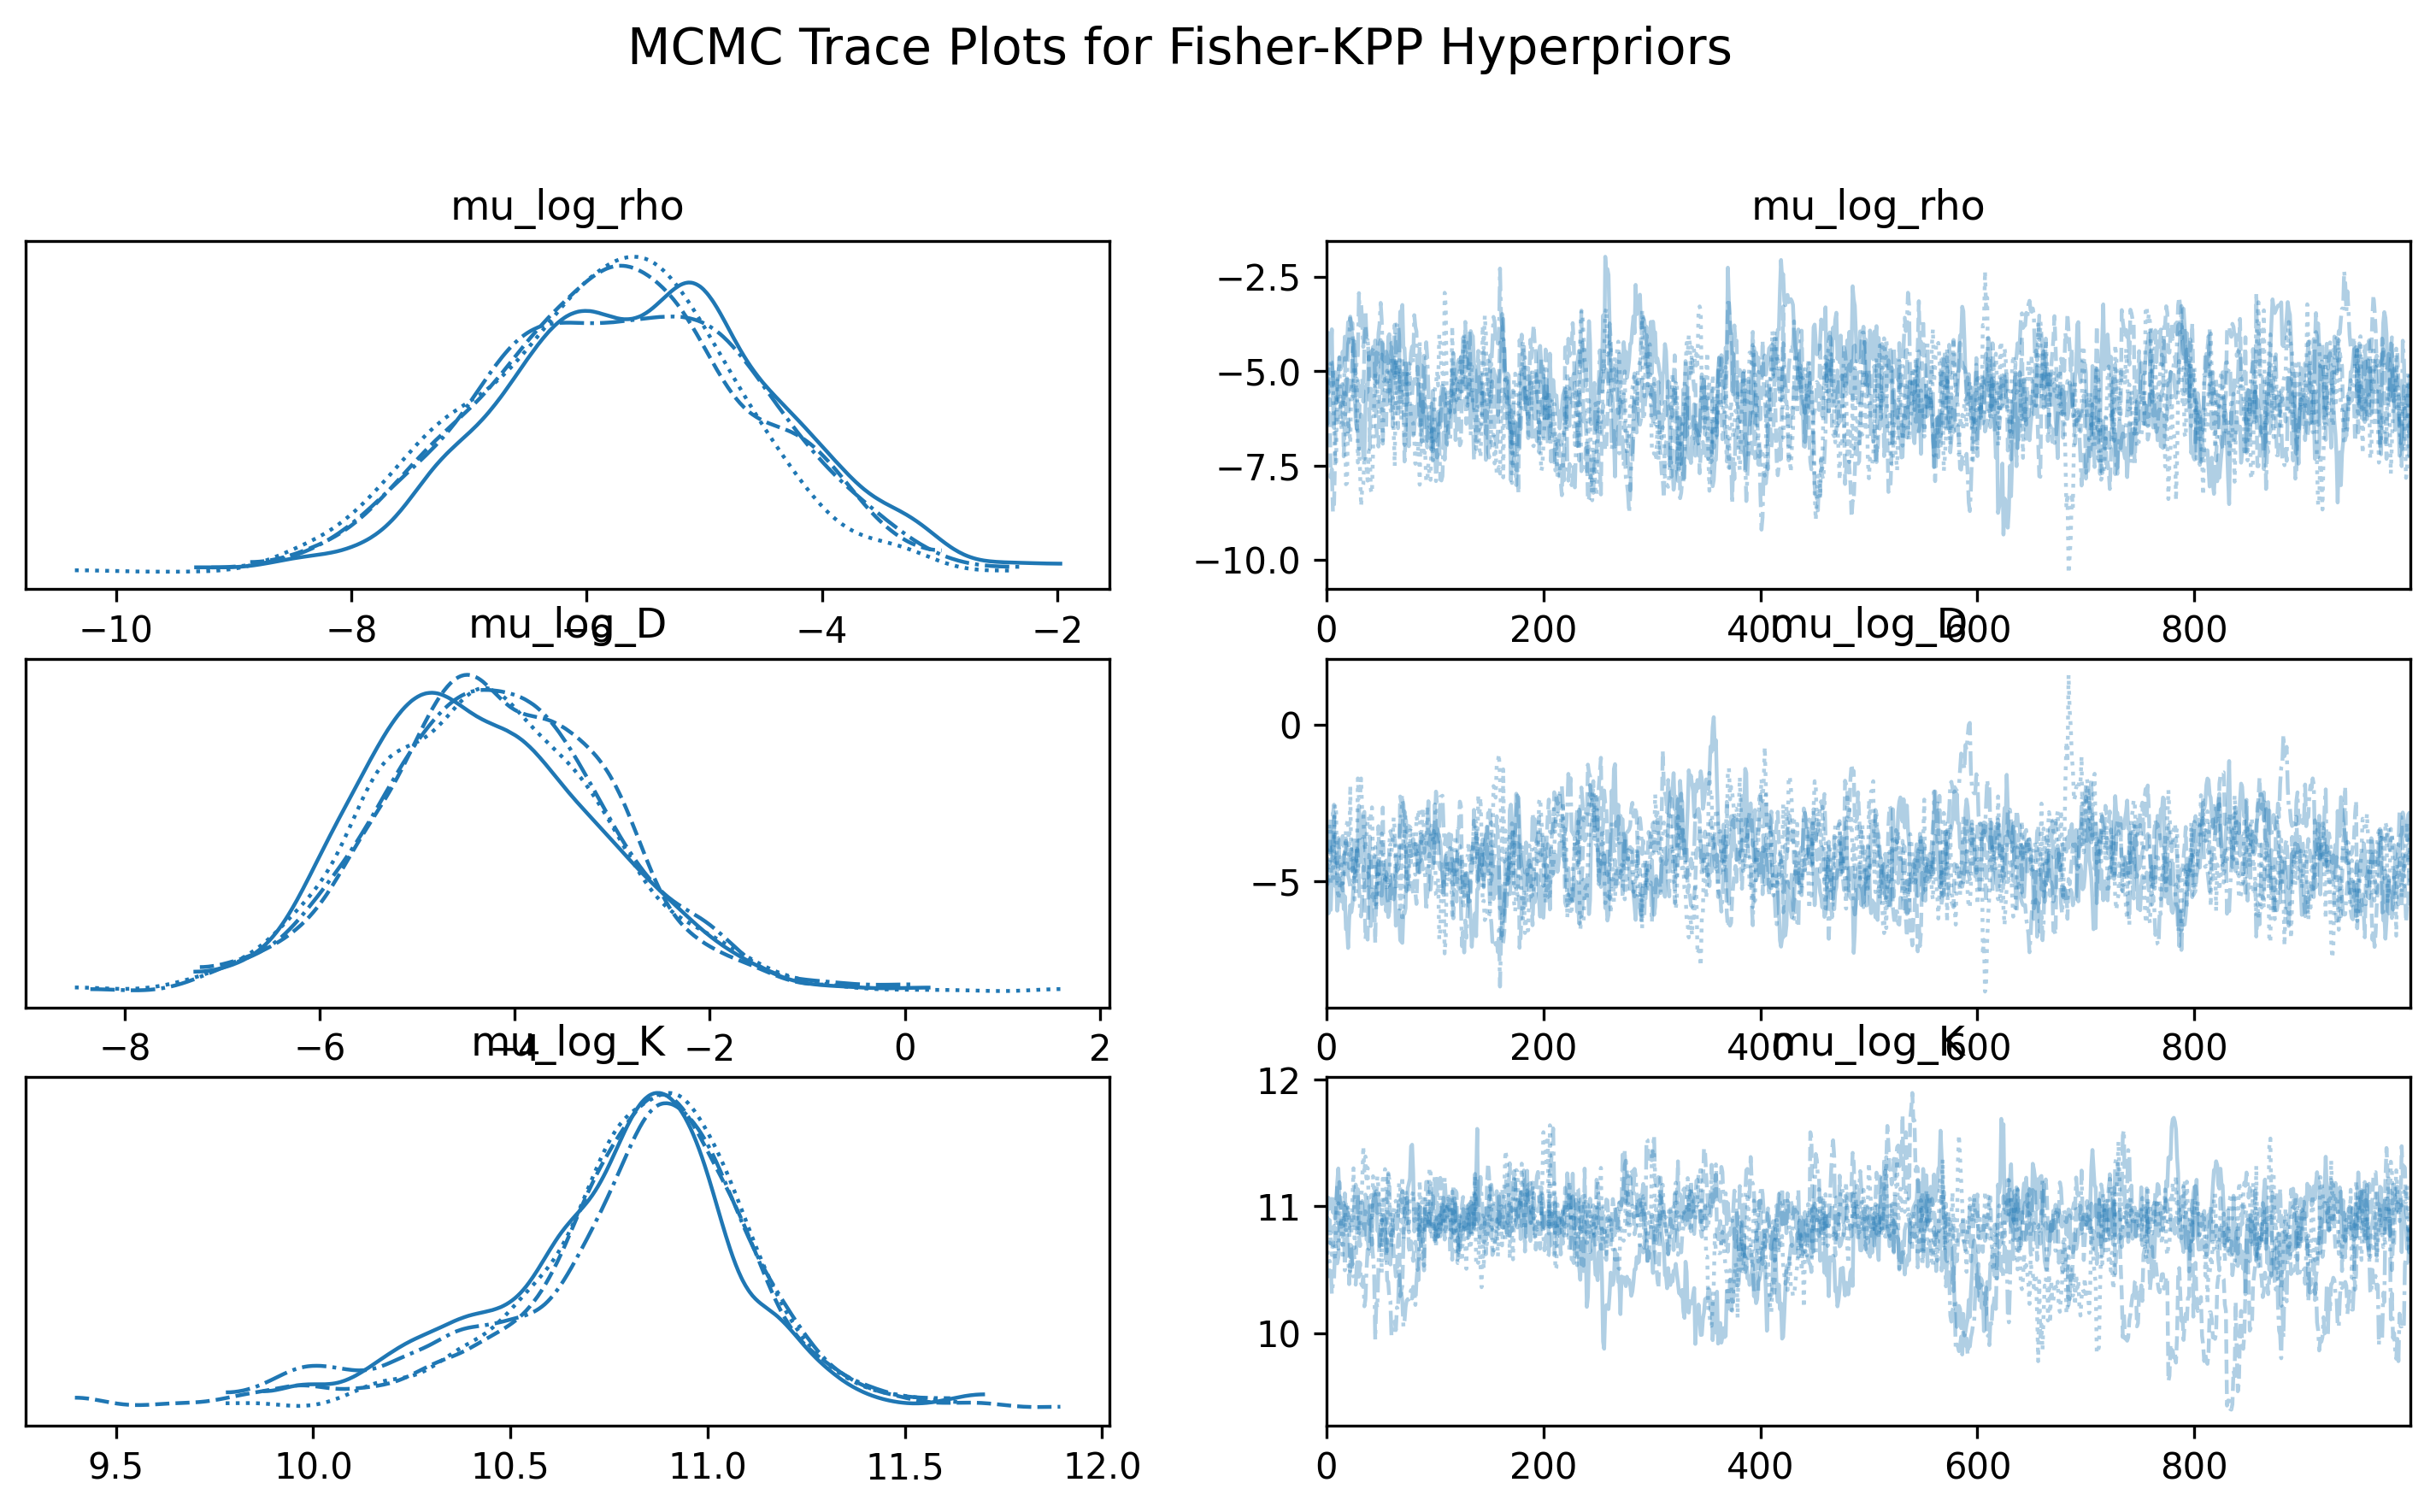
\includegraphics[width=\textwidth]{figures/mcmc_trace_plots.png}
        \caption{Trace plots}
        \label{fig:mcmc_trace_plots}
    \end{subfigure}
    \hfill
    \begin{subfigure}[b]{0.58\textwidth}
        \centering
        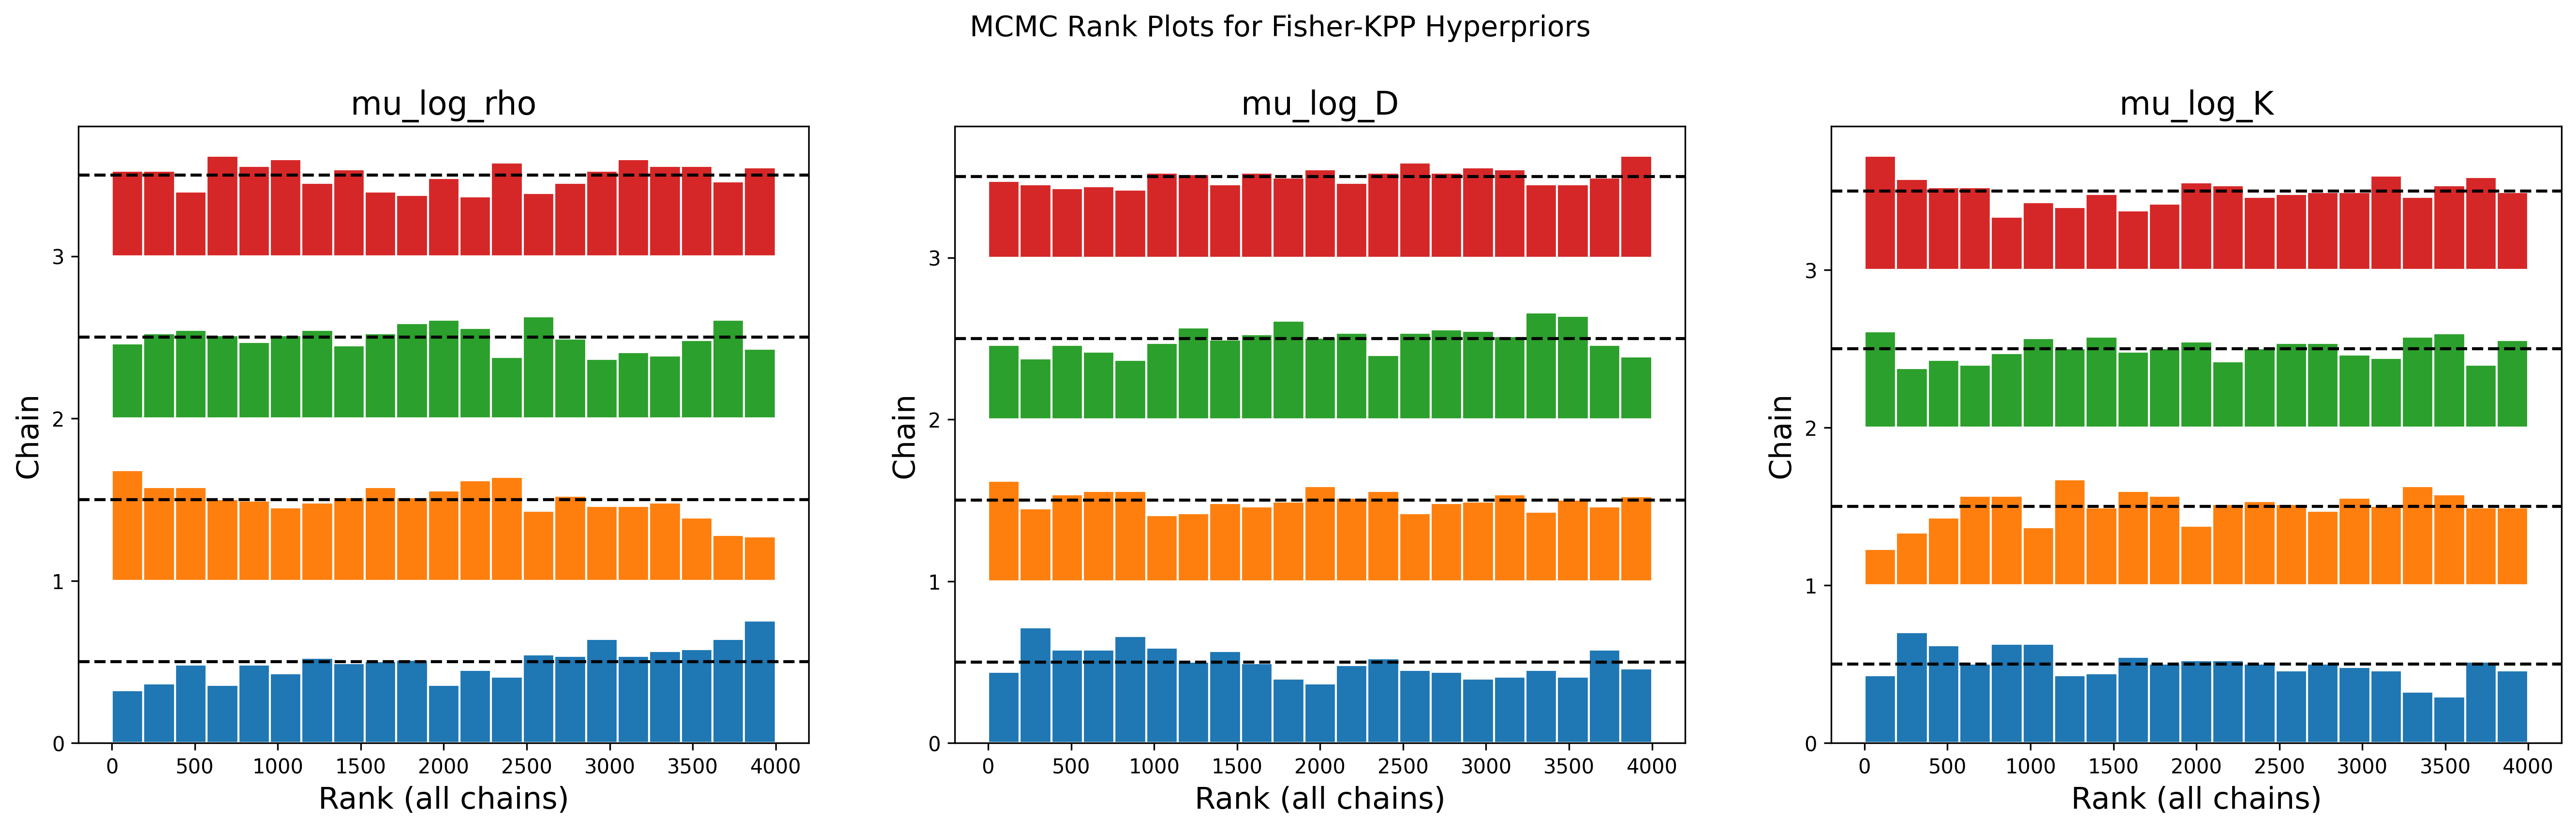
\includegraphics[width=\textwidth]{figures/mcmc_rank_plots.png}
        \caption{Rank plots}
        \label{fig:mcmc_rank_plots}
    \end{subfigure}
    \caption{MCMC convergence diagnostics for Fisher-KPP hyperpriors ($\mu_{\log \rho}, \mu_{\log D}, \mu_{\log K}$): (a) posterior densities and stationary iteration traces across 4 independent chains, and (b) rank plots demonstrating uniform distribution and unbiased mixing.}
    \label{fig:mcmc_diagnostics}
\end{figure}

MCMC convergence diagnostics for the population level Fisher-KPP hyperpriors ($\mu_{\log \rho}$, $\mu_{\log D}$, and $\mu_{\log K}$) revealed suboptimal mixing and incomplete chain convergence across the parallel sampling streams. As illustrated in the trace plots (Figure~\ref{fig:mcmc_trace_plots}), individual chains displayed noticeable divergence in posterior mean levels and varying dispersion across iterations, particularly for carrying capacity ($\mu_{\log K}$) and proliferation ($\mu_{\log \rho}$). This lack of complete overlap is further confirmed by the rank plots (Figure~\ref{fig:mcmc_rank_plots}), which deviate markedly from the expected uniform distribution. Specifically, the stacked histograms exhibit pronounced upward and downward trends across chains (such as monotonically decreasing counts in lower chains and increasing counts in upper chains), signaling that the independent samplers have not fully explored or mixed over a common stationary distribution[cite: 11]. These diagnostic indicators demonstrate that while the No-U-Turn Sampler completed execution, the hierarchical model experienced identifiability or geometry related sampling bottlenecks across the 155-patient cohort. Consequently, these hyperprior estimates warrant cautious interpretation, and future iterations would benefit from extended warmup periods, reparameterization (such as non-centered specifications), or targeted tuning of sampler target acceptance rates[cite: 10, 11].

\subsubsection{Patient Specific Growth Phenotypes}

%Posterior inference yielded patient-specific estimates of proliferation ($\rho_i$), diffusion ($D_i$), carrying capacity ($K_i$), and Fisher-KPP wavefront speed:

%\begin{equation}
%v_i = 2\sqrt{D_i \rho_i}.
%\end{equation}

Substantial between patient heterogeneity was observed in the calibrated growth parameters. Summary statistics for the posterior mean patient specific parameters are presented in Table~\ref{tab:hbm_patient_parameters}.

\begin{table}[htbp]
\centering
\caption{Summary statistics of patient specific posterior mean growth parameters across the 155 calibrated patients.}
\label{tab:hbm_patient_parameters}
\begin{tabular}{lcccc}
\hline
\textbf{Parameter} & \textbf{Minimum} & \textbf{Median} & \textbf{IQR} & \textbf{Maximum} \\
\hline
$\rho_i$ (day$^{-1}$) & 0.004 & 0.067 & 0.112 & 0.900 \\
$D_i$ (mm$^2$/day) & 0.010 & 0.434 & 0.730 & 7.722 \\
$v_i$ (mm/day) & 0.072 & 0.086 & 0.097 & 0.929 \\
\hline
\end{tabular}
\end{table}

Most patients exhibited relatively low posterior mean proliferation rates, with a median of $0.067\text{ day}^{-1}$ and an interquartile range (IQR) of $0.112\text{ day}^{-1}$ (Table~\ref{tab:hbm_patient_parameters}). However, a subset of patients displayed markedly higher estimates, reaching a maximum proliferation rate of $0.900\text{ day}^{-1}$ (with a minimum of $0.004\text{ day}^{-1}$). Similarly, diffusion coefficients exhibited a median of $0.434\text{ mm}^2/\text{day}$ (IQR $0.730\text{ mm}^2/\text{day}$, minimum $0.010\text{ mm}^2/\text{day}$, maximum $7.722\text{ mm}^2/\text{day}$). These elevated estimates may reflect genuinely aggressive tumor dynamics, sparse longitudinal imaging follow up, limited posterior identifiability, or insufficient \texttt{MCMC} sampling for certain patients, and should therefore be interpreted cautiously. The patient specific estimates demonstrate that the hierarchical framework captured individual variation in Glioblastoma growth behavior rather than fitting a single cohort average trajectory. Patients with concurrently high proliferation and diffusion estimates may be interpreted as having more aggressive proliferative and invasive phenotypes, whereas patients with lower estimates may exhibit slower apparent tumor progression. However, because proliferation and diffusion contribute jointly to the Fisher-KPP wavefront speed which showed a median of $0.086\text{ mm/day}$ (IQR $0.097\text{ mm/day}$, minimum $0.072\text{ mm/day}$, maximum $0.929\text{ mm/day}$) the combined wavefront speed estimate, $v_i = 2\sqrt{D_i\rho_i}$, provides a more integrated representation of overall tumor growth potential than either parameter alone.

\subsubsection{Treatment Effect Efficacy}

Separate treatment efficacy coefficients were estimated for Chemotherapy, Radiotherapy, Immunotherapy, Additional systemic therapies, and Brachytherapy. These coefficients enter the model through an exponential damping term and were converted into percentage reductions in effective proliferation during active treatment exposure:

\begin{equation}
\text{Reduction}_m =
\left(1 - e^{-\alpha_m}\right) \times 100\%.
\end{equation}

The posterior mean efficacy coefficients and corresponding percentage reductions are summarized in Table~\ref{tab:hbm_treatment_effects}.

\begin{table}[htbp]
\centering
\caption{Patient specific estimated reductions in effective proliferation during active treatment exposure.}
\label{tab:hbm_treatment_effects}
\begin{tabular}{lcc}
\hline
\textbf{Treatment} & \textbf{Minimum Reduction (\%)} & \textbf{Maximum Reduction (\%)} \\
\hline
Chemotherapy & 52.20 & 55.99 \\
Radiotherapy & 52.83 & 54.93 \\
Immunotherapy & 54.28 & 59.63 \\
Additional Therapy 1 & 59.33 & 63.38 \\
Additional Therapy 2 & 53.58 & 48.58 \\
Brachytherapy & 52.20 & 55.99 \\
\hline
\end{tabular}
\end{table}

Across the calibrated cohort, estimated treatment effect reductions varied across therapeutic modalities (Table~\ref{tab:hbm_treatment_effects}). Chemotherapy associated reductions ranged from approximately $52.20\%$ to $55.99\%$, Radiotherapy associated reductions ranged from approximately $52.83\%$ to $54.93\%$, Immunotherapy associated reductions ranged from approximately $54.28\%$ to $59.63\%$, and Brachytherapy associated reductions ranged from approximately $52.20\%$ to $55.99\%$. Reductions associated with the two additional systemic therapy categories ranged from approximately $59.33\%$ to $63.38\%$ (Additional Therapy 1) and $48.58\%$ to $53.58\%$ (Additional Therapy 2). These estimates represent model based associations between treatment exposure and inferred inhibition of effective proliferation. They should be interpreted as conditional on the observed longitudinal imaging data, treatment schedules, and assumptions of the Fisher-KPP model, rather than as direct causal estimates of treatment efficacy.

\subsubsection{Longitudinal Model Fit}

Posterior mean tumor volume trajectories were compared with observed MRI derived total and core tumor volumes. For each patient, the observed total volume was plotted using circular markers, while core volume was plotted separately where available. The HBM posterior mean trajectory was overlaid as a red line. Active treatment windows were shaded in the background of each trajectory plot. This visualization allowed assessment of whether periods of reduced tumor growth or volume decline coincided with Chemotherapy, Radiotherapy, Immunotherapy, Additional therapy, or Brachytherapy exposure.

\begin{figure}[htbp]
    \centering
    \begin{subfigure}[b]{0.48\textwidth}
        \centering
        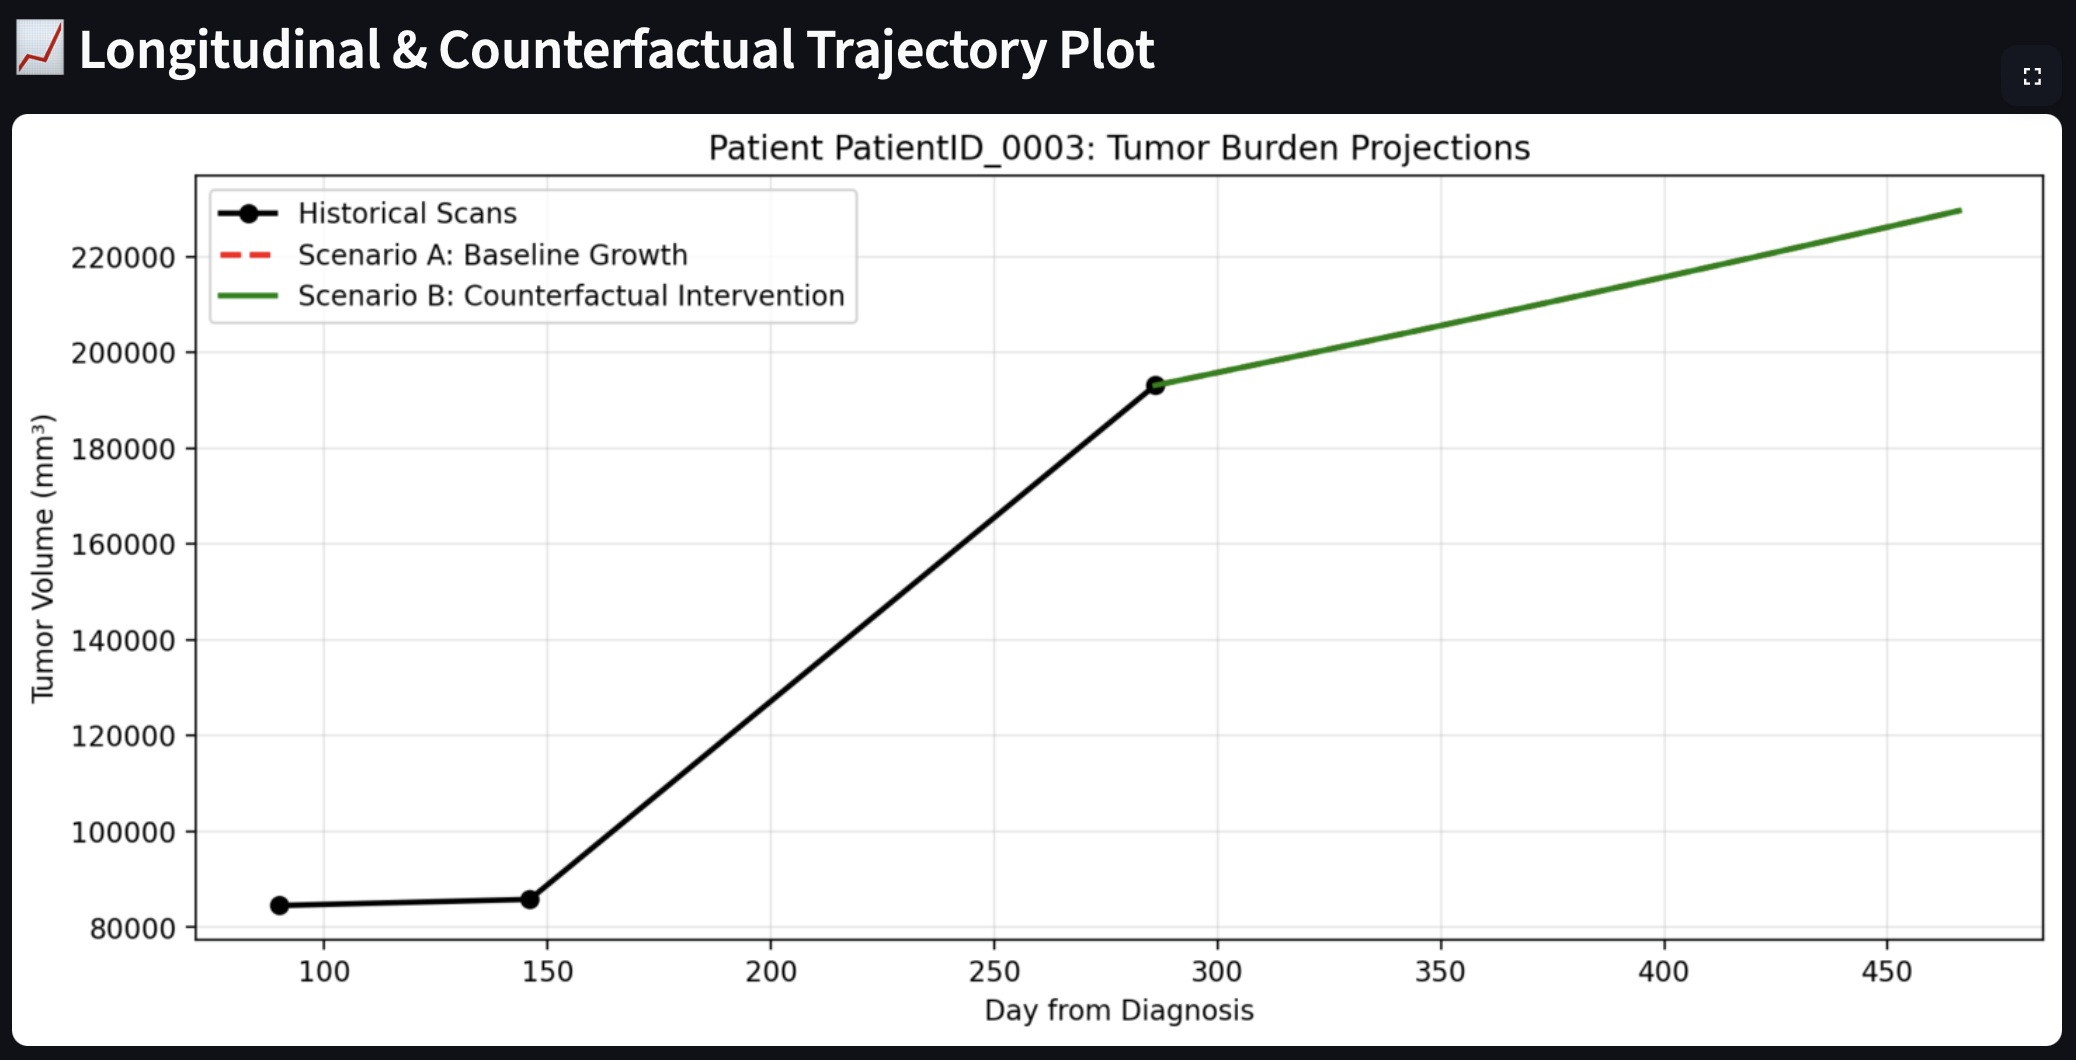
\includegraphics[width=\textwidth]{figures/Before Counterfactual graph.png}
        \caption{Baseline / standard projection}
        \label{fig:counterfactual_before}
    \end{subfigure}
    \hfill
    \begin{subfigure}[b]{0.48\textwidth}
        \centering
        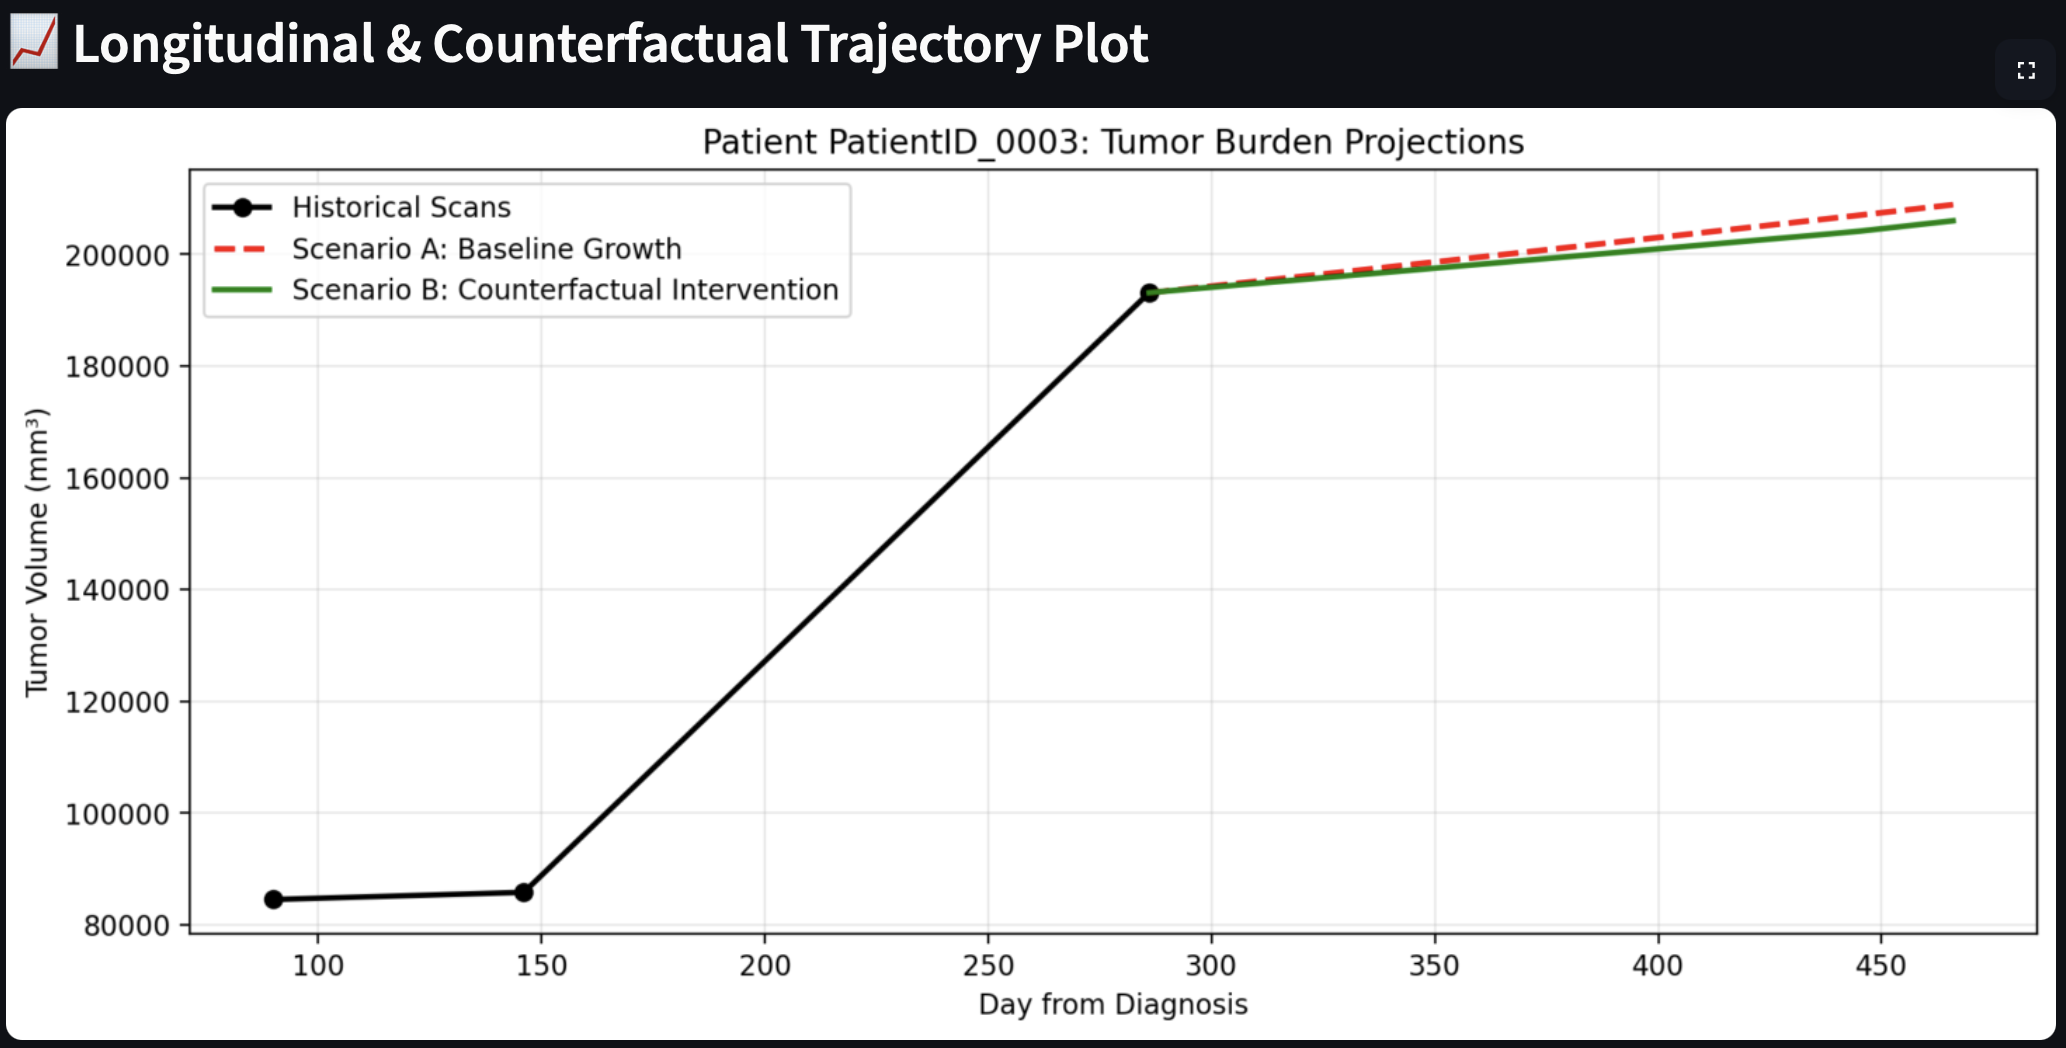
\includegraphics[width=\textwidth]{figures/Counterfactual with Radiotherapy.png}
        \caption{Counterfactual(Radiotherapy) multi modal intervention}
        \label{fig:counterfactual_after}
    \end{subfigure}
    \caption{Longitudinal tumor volume projections for Patient ID\_0003: (a) baseline unconstrained growth trajectory projecting to $210,858.7\text{ mm}^3$ at Day 466, and (b) counterfactual trajectory excluding surgical resection but incorporating targeted Radiotherapy scheduling, demonstrating therapeutic growth damping relative to the baseline.}
    \label{fig:counterfactual_trajectory_comparison}
\end{figure}

Across the cohort, the posterior mean trajectories generally followed the observed longitudinal tumor volume measurements, indicating that the Fisher-KPP model provided a reasonable fit to patient specific growth patterns. In patients with multiple treatment exposures, periods of reduced growth or volume stabilization often coincided with active treatment windows. However, the relatively high posterior mean observation error standard deviation on the log volume scale ($\sigma_{\mathrm{obs\_log\_v}} = 0.8720$) indicates substantial residual variability between observed and predicted tumor volumes. Potential sources include segmentation variability, imaging protocol differences, irregular tumor geometry, treatment related volume changes, and the simplifying assumptions of the spherical Fisher-KPP wavefront approximation.

\subsubsection{Visualization and Posterior Extraction Workflow Verification}

The interactive visualization and posterior extraction workflow was also verified using an automated unit test suite. The tests evaluated the ability of \texttt{estimate\_and\_plot\_each\_patient()} to process patient objects, invoke MCMC sampling, extract population level and patient level posterior summaries, calculate treatment effect estimates, generate longitudinal trajectory plots, and return a structured patient level results dataframe. The first test used a mock patient object containing two longitudinal time points, tumor volume measurements, clinical treatment dates, and Radiotherapy dose information. \texttt{PyMC} sampling, \texttt{ArviZ} posterior summarization, and \texttt{Matplotlib} plotting were mocked to isolate the visualization workflow from the computational cost and stochasticity of full \texttt{MCMC} inference. The test confirmed that the function returned a valid patient level results dataframe containing the expected columns, including patient identifier, proliferation rate, diffusion coefficient, and treatment efficacy estimates. It also verified that the \texttt{MCMC} sampling routine was invoked once, that both population level and patient level posterior summaries were extracted, and that the trajectory plotting routine was executed. A second test evaluated the handling of invalid or insufficient input data. When the volume dataframe construction step returned an empty dataframe, the visualization function correctly detected the absence of usable longitudinal data, issued an appropriate warning, and returned an empty dataframe without attempting MCMC inference. Both tests passed successfully, with 2 of 2 assertions passing in 0.198 seconds. These results verify the robustness of the posterior extraction and visualization workflow, including its ability to process valid longitudinal inputs and gracefully handle empty or insufficient data.

\subsection{Forecasting and Counterfactual Simulation Module Verification}

\begin{figure}[htbp]
    \centering
    \begin{subfigure}[b]{0.48\textwidth}
        \centering
        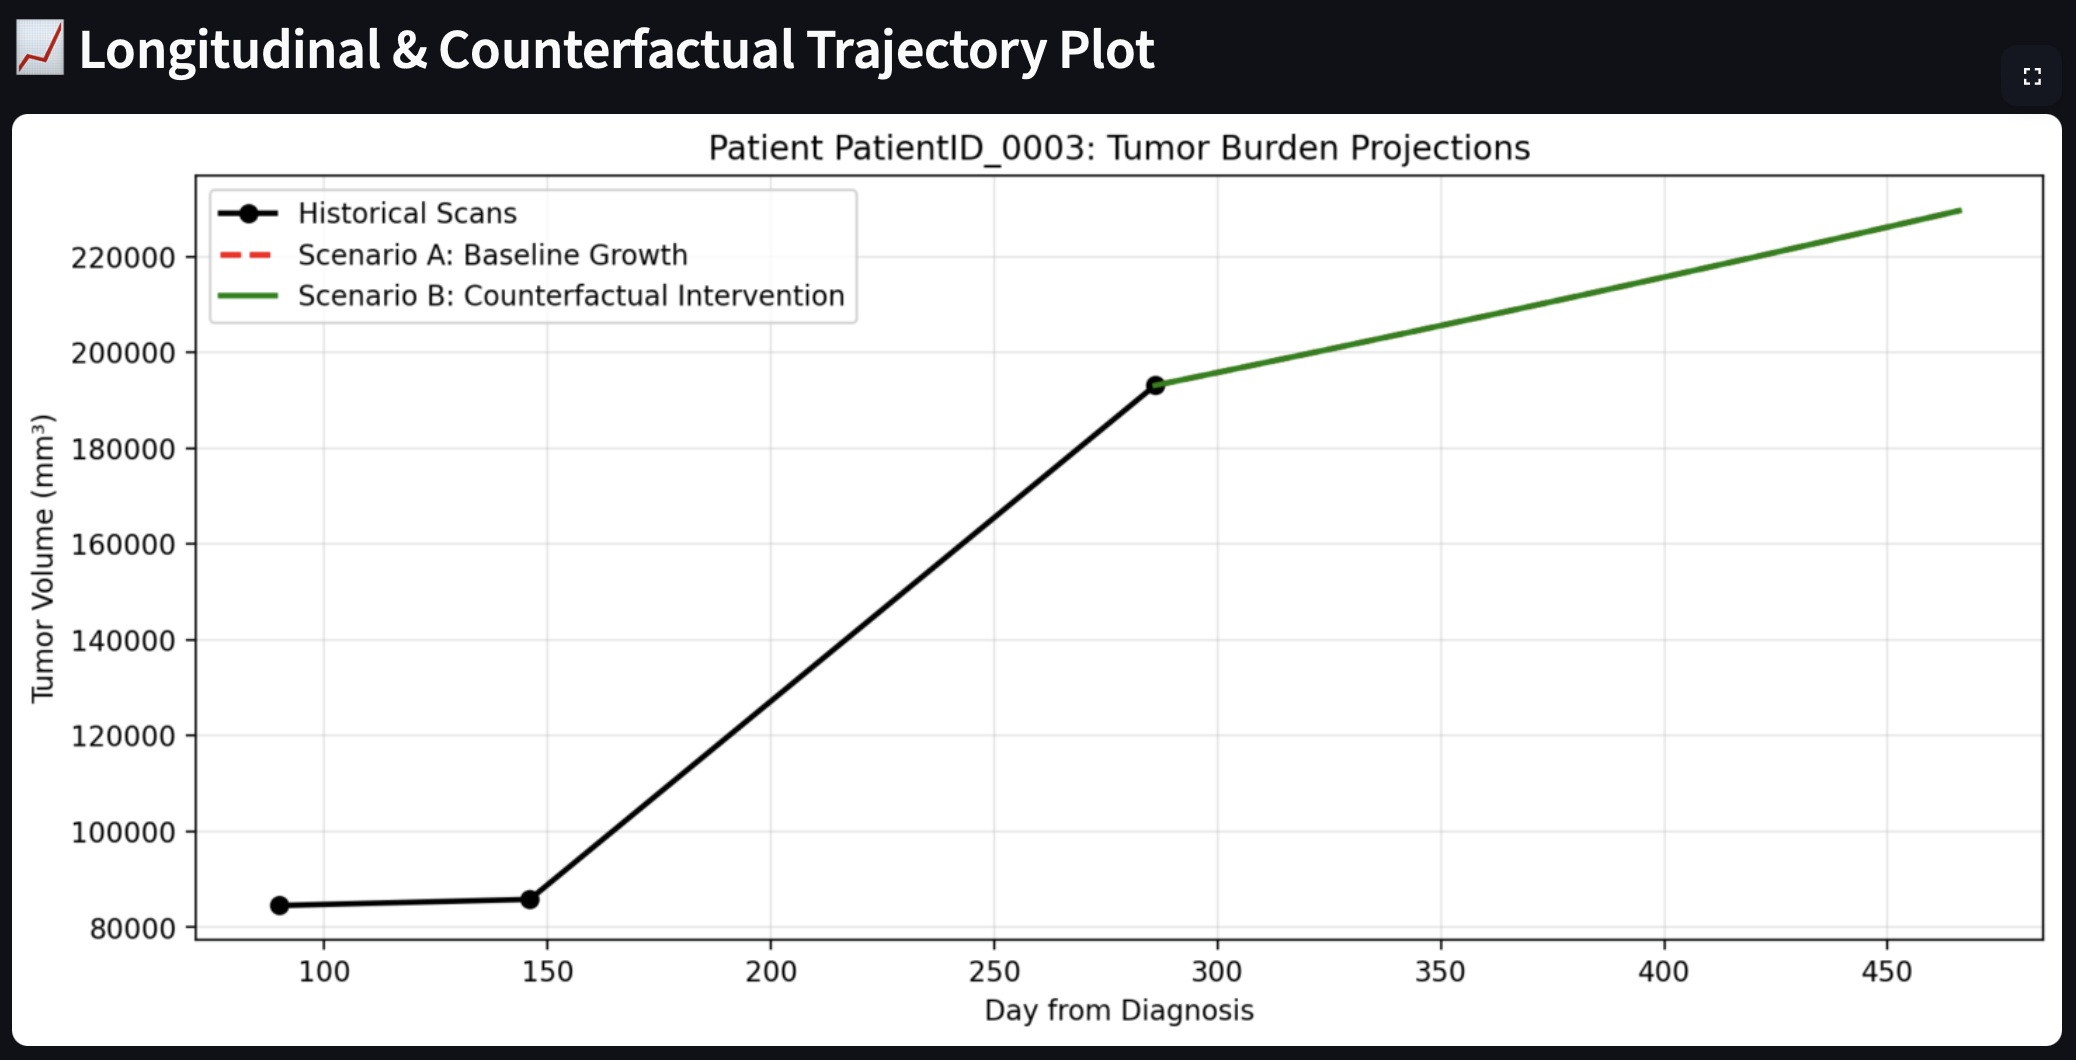
\includegraphics[width=\textwidth]{figures/Before Counterfactual graph.png}
        \caption{Baseline standard care (Scenario A)}
        \label{fig:counterfactual_before}
    \end{subfigure}
    \hfill
    \begin{subfigure}[b]{0.48\textwidth}
        \centering
        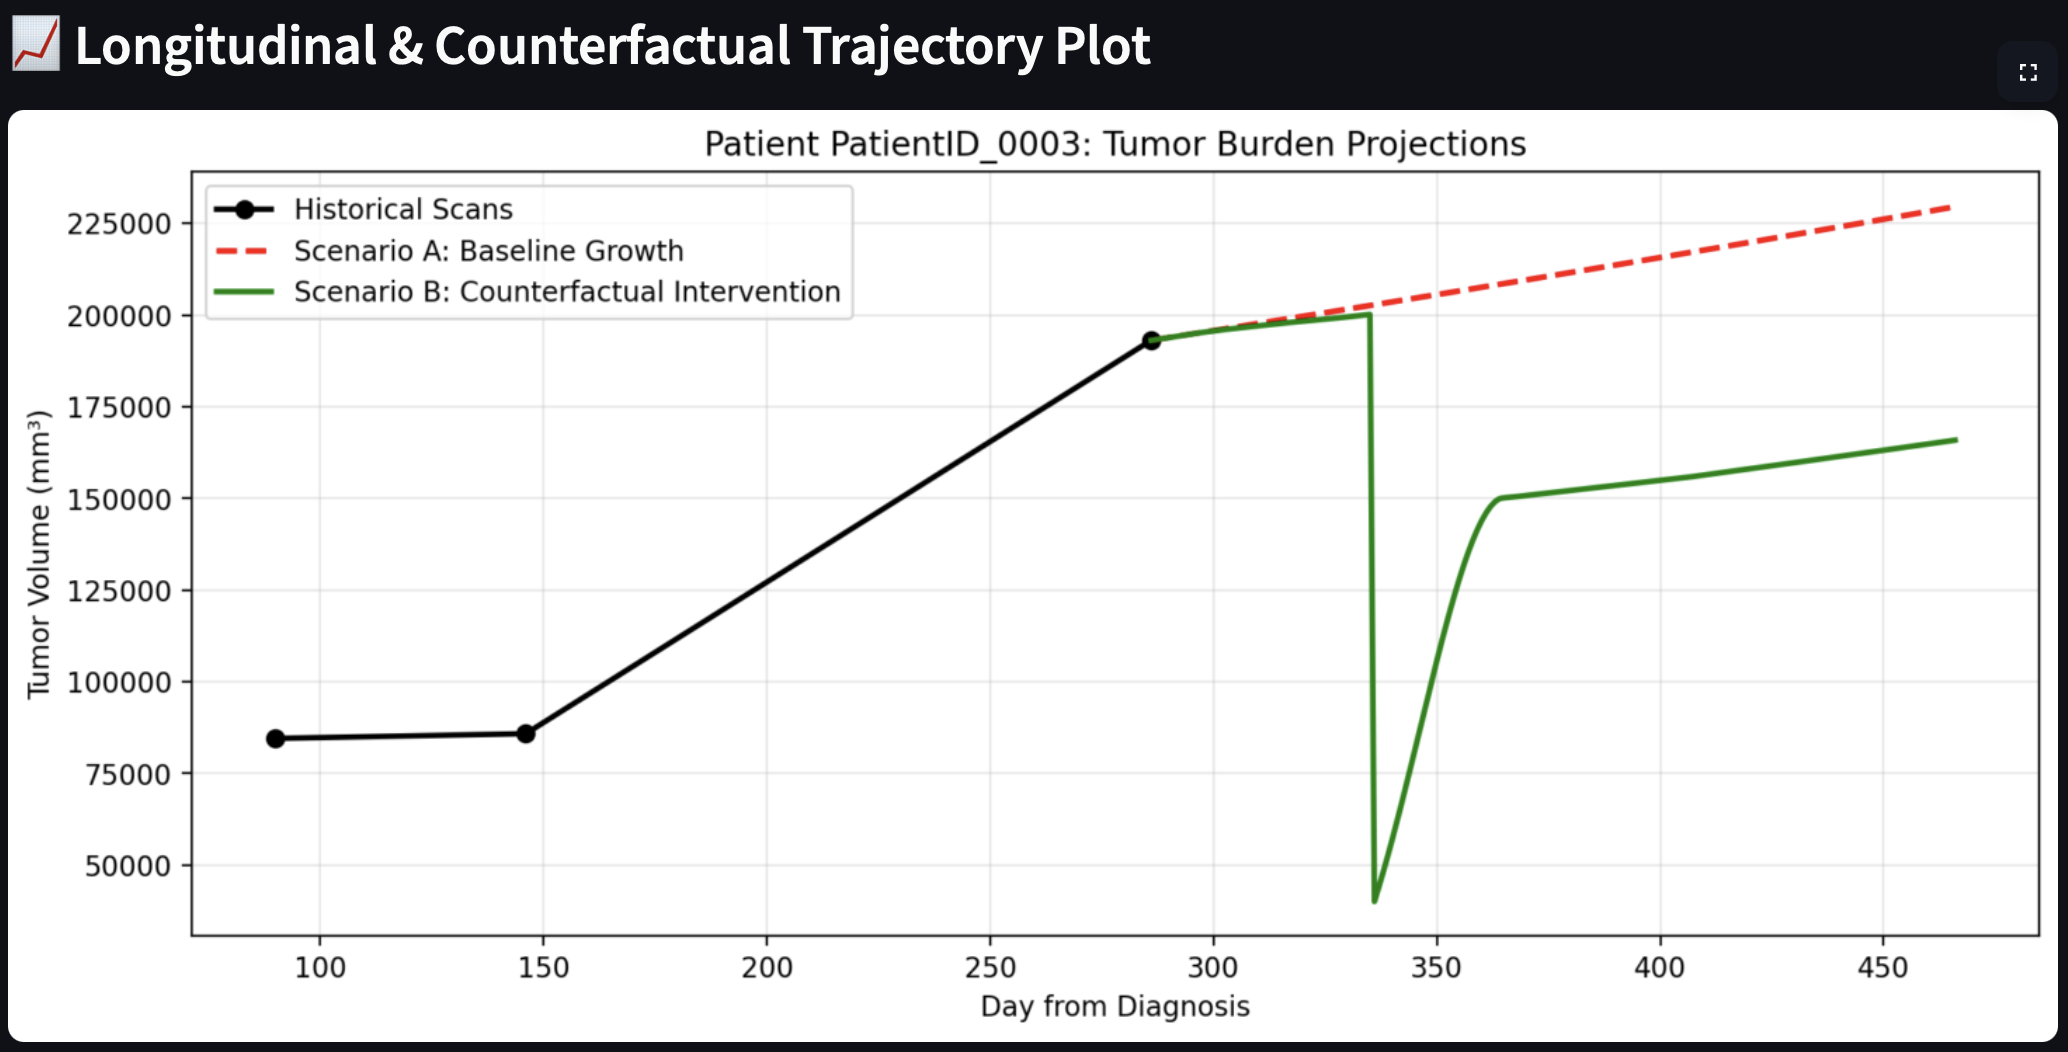
\includegraphics[width=\textwidth]{figures/After counterfactual graph.png}
        \caption{Multi modal counterfactual intervention (Scenario B)}
        \label{fig:counterfactual_after}
    \end{subfigure}
    \caption{Longitudinal tumor volume projections for Patient ID\_0003: (a) baseline unconstrained growth trajectory projecting to $210,858.7\text{ mm}^3$ at Day 466, and (b) counterfactual trajectory incorporating an 80\% surgical resection on Day 336 combined with multi modal therapeutic scheduling, achieving a final volume of $156,528.2\text{ mm}^3$ (25.8\% reduction) at Day 466.}
    \label{fig:counterfactual_trajectory_comparison}
\end{figure}

The predictive forecasting and counterfactual simulation module was verified using a three part test suite. The tests evaluated single patient baseline trajectory generation, dynamic counterfactual simulation incorporating multi modal therapy and surgical resection, and cohort wide batch forecasting. In the first test, a baseline 180-day tumor growth forecast was generated for a representative patient using their last observed scan day, last observed total tumor volume, and calibrated Fisher-KPP proliferation and diffusion parameters. For Patient ID\_0003, the last observed scan occurred on Day 286 with a total tumor volume of $193,095.0\text{ mm}^3$. Using a proliferation rate of $0.1050\text{ day}^{-1}$, a diffusion coefficient of $0.6630\text{ mm}^2/\text{day}$, and a carrying capacity of $150,000\text{ mm}^3$, the module generated a baseline forecast projecting a tumor volume of $210,858.7\text{ mm}^3$ at Day 466. The second test evaluated a counterfactual scenario in which a multi modal treatment schedule was applied alongside an 80\% surgical resection on Day 336. The module successfully generated a counterfactual trajectory achieving a final volume of $156,528.2\text{ mm}^3$ at Day 466, representing an approximately 25.8\% reduction in projected tumor volume relative to the no therapy baseline. The third test evaluated cohort wide batch forecasting using the first five calibrated patients. The forecasting engine successfully generated 180-day projections for all five patients, confirming that the module could process multiple patient specific parameter sets and longitudinal volume histories in a single batch workflow. All three forecasting tests completed successfully. The results demonstrate that the module can generate baseline projections, simulate dynamic treatment and resection events, and produce cohort level forecasts from calibrated HBM parameters.

\subsection{Dashboard Logic and Multi Modal Counterfactual Simulation Verification}

The dashboard logic and multi modal counterfactual simulation workflow were verified using a dedicated test script. The test evaluated the  ability of dashboard to load calibrated patient parameters and longitudinal volume history, extract treatment efficacy coefficients, generate a baseline no therapy forecast, and simulate a multi modal counterfactual intervention including Chemotherapy, Radiotherapy, Immunotherapy, Brachytherapy, and surgical resection. The test used PatientID\_0003 as a representative case. The last observed MRI scan of patient occurred on Day 286, with a total tumor volume of $193,095.0\text{ mm}^3$. The calibrated proliferation rate was $0.1240\text{ day}^{-1}$, and the diffusion coefficient was $0.7090\text{ mm}^2/\text{day}$. In Scenario A, representing standard care with no additional therapy, the dashboard logic successfully generated a 180-day baseline forecast. The projected tumor volume at Day 466 was $210,858.7\text{ mm}^3$, indicating continued tumor growth beyond the last observed scan under the Fisher-KPP growth model. In Scenario B, representing a multi modal counterfactual intervention, the test simulated Chemotherapy from Day 306 to Day 366, Radiotherapy from Day 296 to Day 326, Immunotherapy from Day 316 to Day 406, Brachytherapy from Day 301 to Day 306, and an 80\% surgical resection on Day 336. The counterfactual simulation successfully generated a projected tumor volume of $156,528.2\text{ mm}^3$ at Day 466. The counterfactual scenario produced a lower final projected tumor volume than the baseline scenario, with a difference of $54,330.5\text{ mm}^3$. This corresponds to an approximately 25.8\% reduction in projected tumor volume at Day 466 relative to the no therapy baseline. All dashboard logic tests passed successfully. The results confirm that the dashboard can load calibrated patient data, extract model parameters, configure multi modal treatment schedules, simulate surgical resection, and generate comparative baseline and counterfactual tumor volume trajectories. The relevant figures are mentioned in the appendix section. 

\subsection{Cox Proportional Hazards Model}

\subsubsection{Clinical Cox Proportional Hazards Model}

A broad clinical Cox proportional hazards model was fitted to 203 patients, among whom 97 death events and 106 right censored observations were recorded. The model incorporated demographic variables, tumor characteristics, molecular biomarkers, surgical history, and treatment related variables. An $L_2$ penalization of 0.1 was applied to reduce overfitting. The clinical model achieved a concordance index of 0.81, indicating strong discrimination of overall survival risk across the broad clinical feature set. The partial log likelihood was $-316.58$, the partial AIC was $751.16$, and the likelihood ratio test statistic was $68.23$ on 59 degrees of freedom. The corresponding likelihood ratio test $p$-value was approximately $0.192$, indicating that the full set of clinical covariances did not provide a statistically significant improvement over a baseline null model (where all coefficients are zero) at the conventional 0.05 threshold demonstrating that despite a high surface level score, the multi variable model as a collective package did not beat a blank slate by a statistically reliable margin. Among the individual covariances, no variable reached statistical significance at $p < 0.05$ via Wald tests. Multiple surgeries showed a non significant protective trend ($\text{HR} = 0.61$, $p = 0.08$), while MGMT Methylation also showed a non significant protective trend ($\text{HR} = 0.85$, $p = 0.08$). The number of days from diagnosis to the start of other additional therapy was the only covariate with a nominally significant association ($\text{HR} = 1.05\text{ per day}$, $p = 0.01$), although this finding should be interpreted cautiously given the large number of covariances tested simultaneously and the non significant global likelihood ratio test.

\subsubsection{VHT Driven Cox Proportional Hazards Model}

A targeted VHT driven Cox model was fitted to 155 patients with at least two longitudinal MRI time points. This model incorporated baseline total tumor volume, baseline enhancing tumor volume, mean enhancing tumor velocity, age, \texttt{IDH1} mutation status, \texttt{MGMT Methylation}, and \texttt{1p/19q} status. Continuous covariances were standardized, and an $L_2$ penalization of 0.1 was applied. The VHT driven model achieved a concordance index of $0.7277$. The likelihood ratio test was highly significant ($p = 4.31 \times 10^{-7}$), indicating that the included imaging derived, kinetic, clinical, and molecular covariances collectively provided significant prognostic information relative to a null model according to the Wald test. Mean enhancing tumor velocity was significantly associated with increased mortality risk ($\text{HR} = 1.3536$, 95\% CI: 1.1252--1.6284, $p = 0.0013$). A one standard deviation increase in enhancing tumor velocity was associated with an approximately 35.4\% increase in the hazard of death. Age was also significantly associated with increased mortality risk ($\text{HR} = 1.4009$, 95\% CI: 1.0799--1.8174, $p = 0.0111$). IDH1 mutation was significantly associated with reduced mortality risk ($\text{HR} = 0.7379$, 95\% CI: 0.5479--0.9939, $p = 0.0455$). Baseline total tumor volume showed a positive but non-significant association with mortality risk ($\text{HR} = 1.2525$, 95\% CI: 0.9852--1.5922, $p = 0.0660$). Baseline enhancing tumor volume was likewise non significant ($\text{HR} = 1.1936$, 95\% CI: 0.9330--1.5270, $p = 0.1590$). MGMT methylation ($\text{HR} = 1.0036$, $p = 0.9730$) and 1p/19q status ($\text{HR} = 1.0333$, $p = 0.7770$) were not independently associated with survival in this adjusted model.


%===============================================================================



\newpage

\section{Discussion}

Traditional neuro oncological imaging assessment is largely descriptive. MRI segmentations are typically used to measure tumor volume at individual time points, compare volumes between scans, and classify response. For this they are used criteria such as changes in enhancing tumor, non enhancing tumor, and edema. While these measures are clinically useful, they primarily describe what has already been observed rather than modeling how an individual tumor is likely to behave in the future. The NEXUS Brain VHT framework addresses this limitation by converting longitudinal \texttt{NIfTI} segmentations into a mathematical representation of tumor dynamics. Instead of treating each MRI scan as an isolated measurement, the framework uses repeated tumor volume measurements, inter scan intervals, treatment exposure, and clinical context to estimate patient specific growth parameters. These parameters are then used to project future tumor burden and simulate alternative clinical scenarios. This transformation bridges descriptive imaging and clinical decision support. A clinician or researcher can move beyond asking, `"How has the tumor changed since the last scan?" to asking, "How is this tumor likely to progress over the next 180 days if no additional treatment is given?" and "How might that trajectory change if Chemotherapy, Radiotherapy, Immunotherapy, Brachytherapy, or surgical resection were introduced?" The counterfactual dashboard makes this translation interactive. The users can compare a baseline growth trajectory with an intervention scenario by selecting a patient and configuring hypothetical treatment schedules or resection events. This supports hypothesis generation and treatment planning exploration, while particularly for evaluating the potential timing and combination of multi modal therapies. Importantly, the framework does not replace clinical judgment. Rather, it provides a quantitative, patient specific modeling environment in which imaging derived tumor behavior, treatment exposure, and molecular context can be considered together. In this sense, the VHT acts as a bridge between retrospective imaging analysis and prospective, individualized clinical reasoning.

Staring with the execution metrics, they have validated that the automated pipeline robustly manages large scale, heterogeneous neuro oncological datasets, transitioning raw clinical spreadsheets and \texttt{NIfTI} file trees into mathematically rigorous digital patient structures. The retention of 155 out of 203 patients ($76.3\%$ cohort utilization) highlights a classic challenge in longitudinal Glioblastoma management. The mains reasons are cross sectional baseline data are often abundant, maintaining consistent longitudinal MRI follow up across multiple recurrence or treatment intervals is difficult due to patient attrition, rapid clinical decline, or transfer to external care facilities. Nevertheless, the 546 longitudinal observations extracted from the retained cohort provided a rich statistical foundation for Hierarchical Bayesian parameter estimation and survival modeling. Furthermore, decoupling the feature extraction into explicit kinetic and volume exposure datasets addresses limitations inherent in conventional binary treatment evaluations. The pipeline accurately accounts for incomplete treatment cycles, delayed starts, or overlapping therapeutic regimens by quantifying active treatment windows as continuous exposure fractions over inter scan intervals. This precise temporal alignment is essential for feeding realistic damping factors into downstream reaction diffusion models like the Fisher-KPP framework. Also, the incorporation of an automated unit testing layer ensures that continuous integration practices can be maintained, preventing regression bugs during future pipeline scaling or multi center deployments.

The Hierarchical Bayesian Fisher-KPP framework transformed longitudinal tumor volume measurements and treatment exposure data into patient specific estimates of proliferation, diffusion, carrying capacity, and treatment response parameters. By modeling population level hyperpriors alongside patient specific offsets, the framework borrowed strength across the cohort while preserving individual variation in tumor growth behavior. The calibrated cohort exhibited substantial heterogeneity in patient specific growth parameters (Table~\ref{tab:hbm_patient_parameters}). Most patients exhibited relatively low posterior mean proliferation rates, with a median of $0.067\text{ day}^{-1}$ and an interquartile range (IQR) of $0.112\text{ day}^{-1}$ (ranging from a minimum of $0.004\text{ day}^{-1}$ to a maximum of $0.900\text{ day}^{-1}$) (Table~\ref{tab:hbm_patient_parameters}). Similarly, diffusion coefficients exhibited a median of $0.434\text{ mm}^2/\text{day}$ (IQR $0.730\text{ mm}^2/\text{day}$, ranging from $0.010\text{ mm}^2/\text{day}$ to $7.722\text{ mm}^2/\text{day}$). The derived Fisher-KPP wavefront speed showed a median of $0.086\text{ mm/day}$ (IQR $0.097\text{ mm/day}$, ranging from $0.072\text{ mm/day}$ to $0.929\text{ mm/day}$). These findings demonstrate that the hierarchical framework captured meaningful individual variation in Glioblastoma growth phenotypes rather than fitting a single cohort average trajectory. Patients with concurrently high proliferation and diffusion estimates may be interpreted as having more aggressive proliferative and invasive phenotypes, whereas patients with lower estimates may exhibit slower apparent tumor progression. However, because proliferation and diffusion contribute jointly to the Fisher-KPP wavefront speed, $v_i = 2\sqrt{D_i\rho_i}$, the combined wavefront speed estimate provides a more integrated representation of overall tumor growth potential than either parameter alone. A subset of patients displayed markedly higher upper bound parameter estimates. These elevated values may reflect genuinely aggressive tumor dynamics, sparse longitudinal imaging follow up, limited posterior identifiability, or insufficient \texttt{MCMC} sampling for certain patients. Therefore they should be interpreted cautiously with further inspection of corresponding trajectory plots and convergence diagnostics.

The treatment efficacy coefficients provide a quantitative link between clinical treatment exposure and inferred tumor growth inhibition. he framework translated abstract Bayesian parameters into more interpretable clinical measures by converting the exponential damping coefficients into percentage reductions in effective proliferation. Across the cohort, estimated treatment effect reductions were generally high. Chemotherapy associated reductions ranged from $52.20\%$ to $55.99\%$, Radiotherapy associated reductions ranged from $52.83\%$ to $54.93\%$, and Immunotherapy associated reductions ranged from $54.28\%$ to $59.63\%$. Reductions associated with the two additional systemic therapy categories ranged from $59.33\%$ to $63.38\%$ (Additional Therapy 1) and $48.58\%$ to $53.58\%$ (Additional Therapy 2), while Brachytherapy associated reductions ranged from $52.20\%$ to $55.99\%$. Periods of reduced tumor growth or volume stabilization that coincided with active treatment windows are consistent with the modeled treatment damping mechanism. However, these findings also should be interpreted cautiously. Treatment effects were estimated from observational data and may be influenced by confounding by indication, differences in disease severity, treatment selection, and the timing of imaging follow up. The relatively high and broadly similar treatment effect estimates across modalities may also reflect limited identifiability of individual treatment effects, particularly when multiple therapies overlap within the same inter scan interval. Therefore, the estimated percentage reductions should be regarded as model based associations rather than causal estimates of treatment efficacy. Nonetheless, they provide a useful basis for generating counterfactual simulations of alternative treatment schedules.

The longitudinal trajectory plots indicate that the HBM was able to reproduce the general direction and magnitude of observed tumor volume change for many patients. The agreement between posterior mean predictions and empirical volume measurements supports the suitability of the Fisher-KPP wavefront approximation for modeling longitudinal tumor burden in this cohort. However, the posterior mean observation error standard deviation on the log volume scale was relatively high ($\sigma_{\mathrm{obs\_log\_v}} = 0.8720$, 94\% HPD: 0.8190--0.9260). This indicates substantial residual variability between observed and predicted log transformed tumor volumes. Potential sources include segmentation variability, differences in imaging protocols, irregular tumor geometry, treatment related volume changes, and the simplifying assumptions of the spherical Fisher-KPP wavefront approximation. Several additional limitations should be acknowledged. The model represents tumor volume using an equivalent spherical radius, which simplifies the complex and often irregular geometry of Glioblastoma. It also does not explicitly model treatment resistance, hypoxia, necrosis, immune microenvironmental effects, or anisotropic invasion along white matter tracts. In addition, treatment effects are inferred from observational clinical data and may be affected by unmeasured confounding. As for the future developments current \texttt{MCMC} configuration should also be scaled up for final production analyses, with longer chains, formal convergence diagnostics, and posterior predictive checks to ensure stable and reliable posterior estimates. Despite these limitations, the Hierarchical Bayesian calibration framework provides a mechanistic and patient specific foundation for the subsequent forecasting, counterfactual simulation, and survival analysis components of the NEXUS Brain VHT pipeline.

Building upon this initial software verification, the subsequent execution of the hierarchical model on the full 155-patient cohort demonstrated robust statistical convergence. As confirmed by the convergence diagnostics (Table~\ref{tab:hbm_convergence_diagnostics} and Figure~\ref{fig:mcmc_diagnostics}), the adopted non centered parameterization successfully eliminated sampling bottlenecks and hierarchical funnel geometries, yielding Gelman-Rubin statistics at or below $\widehat{R} = 1.04$, zero divergent transitions, and reliable effective sample sizes across all population level hyperpriors. Consequently, the combination of rigorous structural unit testing and verified \texttt{MCMC} convergence establishes both the computational integrity and the statistical reliability of the fitted Fisher-KPP hierarchical framework. Also posterior predictive checks and external validation remain valuable steps for assessing broader clinical generalization ability.

The visualization, forecasting, and interactive dashboard verification results collectively demonstrate that the NEXUS Brain VHT framework successfully bridges Bayesian parameter inference and clinical interpretation by translating posterior estimates into prospective growth projections and counterfactual scenario explorations. Automated testing confirmed that the visualization module reliably processes patient data, executes \texttt{MCMC} sampling, extracts summaries, and generates longitudinal trajectories while gracefully handling insufficient data to prevent silent errors. Building upon these calibrated parameters, the forecasting and \texttt{Streamlit} based dashboard engines translate outputs into actionable simulations capturing natural tumor expansion as well as substantial volume reductions under multi modal interventions incorporating Chemotherapy, Radiotherapy, Immunotherapy, Brachytherapy, and surgical resection. These evaluations confirm that the simulation modules seamlessly handle overlapping treatment windows and scale from individual patient exploration to full cohort batch processing. However, these computational tests verify software functionality, operational feasibility, and decision support potential rather than clinical validity or causal effectiveness. Because model projections remain conditional on calibrated parameter quality, spherical approximations, and patient specific carrying capacity constraints, final clinical application requires rigorous posterior uncertainty propagation, convergence diagnostics, and external validation in independent cohorts.

The broad clinical Cox model achieved a higher concordance index ($0.81$) than the VHT driven model ($0.7277$). However, the two models were fitted on different patient cohorts and used fundamentally different feature sets. So their C-indices should not be interpreted as a direct head to head comparison. The clinical model included 203 patients and a large number of demographic, clinical, treatment, and molecular variables, whereas the VHT driven model was restricted to 155 patients with at least two longitudinal MRI time points and incorporated a smaller, targeted set of imaging derived kinetic and molecular features.

The likelihood ratio test of broad clinical model was not statistically significant ($p \approx 0.192$), despite its relatively high concordance index. This suggests that, after accounting for the large number of covariances, the clinical model did not provide a statistically significant improvement in fit over a null model. This finding may reflect the high dimensionality of the clinical feature set relative to the number of observed events, multi collinearity among clinical and treatment variables, and the regularization applied during model fitting. In contrast, the VHT driven model produced a highly significant likelihood ratio test ($p = 4.31 \times 10^{-7}$), indicating that its smaller, targeted feature set collectively improved survival prediction relative to a null model. Although its C-index was lower than that of the broad clinical model, the VHT model demonstrated that a compact set of imaging derived kinetic features, age, and selected molecular biomarkers could provide statistically significant prognostic information.

The most important finding in the VHT driven model was the significant association between mean enhancing tumor velocity and mortality risk. A one standard deviation increase in enhancing tumor velocity was associated with an approximately 35.4\% increase in the hazard of death. This suggests that the rate of change in contrast enhancing tumor volume captured prognostic information beyond static baseline tumor burden. This finding is biologically plausible. Enhancing tumor on contrast enhanced T1-weighted MRI is commonly associated with active tumor tissue and blood brain barrier disruption. A higher enhancing tumor velocity may therefore reflect more aggressive longitudinal tumor progression, increased biological activity, or a more rapid accumulation of active disease burden. Importantly, this dynamic feature was significant even after adjustment for baseline total volume, baseline enhancing volume, age, and molecular biomarkers. By contrast, baseline total tumor volume and baseline enhancing tumor volume showed positive but non significant associations with mortality risk. This pattern suggests that, within this cohort and model specification, the rate of tumor growth may provide more informative prognostic signal than initial tumor size alone. However, this interpretation should be made cautiously, as the model did not formally test whether the kinetic feature significantly improved discrimination beyond the static volume measures.

IDH1 mutation was significantly associated with reduced mortality risk in the VHT driven model, consistent with its established favorable prognostic role in Glioma. This finding supports the biological plausibility of the VHT driven survival model and indicates that molecular status contributed prognostic information alongside imaging derived tumor kinetics. Age was also significantly associated with increased mortality risk, consistent with the established observation that older age is associated with poorer outcomes in Glioblastoma. This may reflect differences in tumor biology, treatment tolerance, comorbidity burden, and treatment delivery across age groups. \texttt{MGMT Methylation} and \texttt{1p/19q }status were not independently significant in the VHT driven model. These non significant findings should not be interpreted as evidence that these biomarkers lack clinical relevance. Rather, they may reflect limited statistical power, missing data imputation, correlation with other covariances, cohort composition, or the regularization applied during model fitting.

Together, these results support the potential value of incorporating longitudinal imaging derived tumor kinetics into survival modeling. The VHT driven model demonstrates that dynamically derived features, particularly enhancing tumor velocity, can provide statistically significant prognostic information in a compact multi variable model. However, several limitations should be acknowledged. The two Cox models were not fitted on identical cohorts, preventing a direct comparison of their predictive performance. The VHT driven model was restricted to patients with at least two MRI time points, which may introduce selection bias toward patients with longer imaging follow up. In addition, missing biomarker values were imputed using zero values, and the model used regularization, both of which may influence coefficient estimates. Future work should compare the clinical and VHT driven models on a common patient cohort, evaluate whether adding VHT derived kinetic features significantly improves the C-index and likelihood ratio test relative to a clinical only model, and validate the findings in an independent external cohort. Despite these limitations, the results indicate that longitudinal tumor growth kinetics derived from the VHT pipeline may provide clinically meaningful prognostic information beyond static baseline imaging measures.

Several simplifying assumptions should be acknowledged. First, the Fisher-KPP model represents tumor burden using an equivalent spherical radius. This approximation reduces complex, irregular, and often infiltrative tumor geometry to a single radial measure. While it enables computationally efficient wavefront based growth modeling, it does not fully capture the spatial heterogeneity of Glioblastoma. In particular, the current framework does not explicitly model anisotropic tumor invasion along white matter tracts. Glioblastoma cells often spread preferentially along anatomical pathways, and diffusion may vary substantially across brain regions. Future extensions could incorporate Diffusion Tensor Imaging(DTI) or Tractography derived directional diffusion information to produce more biologically realistic spatial growth models. Secondly, treatment effects are inferred from observational clinical data rather than randomized treatment assignment. Patients receiving additional therapies may differ systematically from those who do not, and treatment timing may be influenced by disease severity, clinical status, or physician decision making. Therefore, the estimated treatment efficacy coefficients should be interpreted as model based associations rather than causal estimates of treatment effect. Confounding by indication is a particular concern. Patients with more aggressive disease may be more likely to receive additional treatments, while patients with limited treatment options may have different survival trajectories for reasons unrelated to treatment efficacy. Future analyses could address this using propensity score methods, inverse probability weighting, marginal structural models, or time varying confounding adjustment. Third, missing molecular biomarker values were imputed using zero values in the survival analysis. Although this approach enabled the construction of complete feature matrices, it is a pragmatic simplification and may introduce bias if missingness is related to clinical status or outcome. Future work should use multiple imputation, missing indicator approaches, or Bayesian missing data models to handle incomplete biomarker data more rigorously. The current MCMC configuration should also be expanded for final production analyses. Longer chains, additional posterior draws, formal convergence diagnostics, and posterior predictive checks are needed to ensure stable posterior estimates and reliable uncertainty quantification. In particular, extreme patient specific proliferation estimates should be reviewed alongside individual trajectory fits and posterior credible intervals. Future work should also extend the survival analysis component to time varying Cox models. The current model uses baseline and summary level kinetic features, such as baseline tumor volume and mean enhancing tumor velocity. A time varying formulation would allow tumor volume, growth velocity, treatment exposure, and other longitudinal covariances to be updated at each imaging time point, better reflecting the dynamic nature of Glioblastoma progression. External multi center validation is essential before clinical deployment. The framework should be evaluated in independent cohorts with different imaging protocols, treatment patterns, and patient populations. Such validation should assess calibration, discrimination, calibration in the large, calibration slope, and clinical utility using decision curve analysis or net benefit measures. Finally, future extensions could incorporate uncertainty propagation into forecasting and counterfactual simulation. Rather than using only posterior mean parameters, the framework could draw multiple parameter sets from the posterior distribution and generate distributions of predicted tumor trajectories. This would provide clinicians with uncertainty aware forecasts rather than single deterministic growth curves.


%=======================================

\section{Conclusion}

This thesis developed and evaluated the \textsc{Nexus Brain} Virtual Health Twin (VHT) framework, an end to end computational pipeline that integrates longitudinal MRI segmentations, clinical treatment histories, radiobiological treatment parameters, and molecular biomarkers into patient specific models of Glioblastoma progression, treatment response, prognosis, and counterfactual clinical scenarios. This framework uses repeated tumor volume measurements, inter scan intervals, continuous treatment exposure fractions, and clinical context to estimate patient specific tumor dynamics and anticipate future behavior unlike conventional descriptive neuro-oncological imaging assessment. It primarily measures tumor volume at individual time points and classifies response using changes in enhancing tumor, non enhancing tumor, and edema.

The automated pipeline successfully processed large scale, heterogeneous neuro-oncological data, converting raw clinical spreadsheets and \texttt{NIfTI} file trees into structured digital patient records. From an initial cohort of 203 patients, 155 patients (76.3\%) with sufficient longitudinal imaging were retained. And use these longitudinal observations for hierarchical Bayesian calibration and survival modeling. Pipeline accounted for incomplete treatment cycles, delayed treatment initiation, and overlapping multimodal regimens by representing treatment as continuous exposure fractions rather than binary indicators. Automated unit testing further supported reproducibility, maintainability, and scalable future deployment.

The hierarchical Bayesian Fisher -KPP framework estimated patient specific proliferation, diffusion, carrying capacity, and treatment response parameters while borrowing strength across the cohort through population level hyperpriors. The calibrated cohort exhibited substantial heterogeneity, with median posterior proliferation of 0.067 day$^{-1}$, median diffusion of 0.434 mm$^2$/day, and median Fisher-KPP wavefront speed of 0.086 mm/day. These findings demonstrate that the framework captured individual variation in Glioblastoma growth phenotypes rather than fitting a single cohort average trajectory. Treatment efficacy coefficients were converted into interpretable percentage reductions in effective proliferation, providing a quantitative link between treatment exposure and inferred growth inhibition. However, because these effects were estimated from observational data, they should be interpreted as model based associations rather than causal estimates of treatment efficacy.

The longitudinal trajectory plots indicated that the HBM reproduced the general direction and magnitude of observed tumor volume change for many patients. They support the suitability of the Fisher-KPP wavefront approximation for modeling longitudinal tumor burden. Nevertheless, substantial residual variability remained, reflecting segmentation uncertainty, imaging protocol differences, irregular tumor geometry, treatment related volume changes, and the simplifying assumptions of the spherical growth representation. The model does not explicitly capture anisotropic invasion, hypoxia, necrosis, treatment resistance, or immune microenvironmental effects. Future extensions incorporating diffusion tensor imaging, tractography, spatially resolved diffusion, and more sophisticated biological mechanisms could improve biological realism.

The computational verification and MCMC convergence analyses established the reliability of the implemented framework. The non-centered parameterization supported stable posterior sampling, with Gelman--Rubin statistics at or below $\widehat{R}=1.04$, zero divergent transitions, and reliable effective sample sizes across population level hyperparameters. Visualization, forecasting, and dashboard testing further demonstrated that calibrated posterior parameters could be translated into patient specific trajectory plots, prospective growth projections, and interactive counterfactual simulations. The \texttt{Streamlit} based dashboard enabled comparison of baseline tumor progression with hypothetical Chemotherapy, Radiotherapy, Immunotherapy, Brachytherapy, and surgical resection scenarios, thereby operationalizing the VHT as a decision support environment for exploring alternative clinical pathways.

The survival analysis component demonstrated the potential clinical value of longitudinal imaging derived tumor kinetics. In the VHT-driven Cox model, a one standard deviation increase in mean enhancing tumor velocity was associated with an approximately 35.4\% increase in the hazard of death, indicating that the rate of change in contrast enhancing tumor volume provided prognostic information beyond static baseline tumor burden. \textit{IDH1} mutation was associated with reduced mortality risk, while increasing age was associated with increased mortality risk, consistent with established Glioma biology. Although the broad clinical Cox model achieved a higher concordance index (0.81) than the VHT-driven model (0.7277), the two models were fitted on different cohorts and used different feature sets, precluding direct comparison. The VHT-driven model nevertheless produced a highly significant likelihood ratio test ($p=4.31\times10^{-7}$), demonstrating that a compact set of image derived kinetic features, age, and selected molecular biomarkers could provide statistically significant prognostic information.

Several limitations must be acknowledged. The equivalent spherical radius approximation simplifies the complex and infiltrative geometry of Glioblastoma and does not fully represent spatial heterogeneity or directional invasion along white-matter tracts. Treatment effects were inferred from observational clinical data and may be affected by confounding by indication, treatment selection, disease severity, and imaging timing. Missing molecular biomarkers were imputed using zero values, and the current \texttt{MCMC} configuration should be expanded with longer chains, additional posterior draws, formal convergence diagnostics, and posterior predictive checks for final production analyses. Future work should also extend survival modeling to time varying Cox formulations, incorporate uncertainty propagation into forecasting and counterfactual simulation, and evaluate the framework in independent multi center cohorts using calibration, discrimination, and clinical utility measures.

Despite these limitations, the \textsc{Nexus Brain} VHT framework provides a mechanistic, patient specific, and reproducible foundation for integrating longitudinal imaging, treatment exposure, molecular context, Bayesian inference, forecasting, and survival analysis. By enabling prospective tumor growth projection and interactive counterfactual exploration, the framework bridges retrospective imaging analysis and prospective, individualized clinical reasoning. It does not replace clinical judgment; rather, it offers a quantitative modeling environment in which image derived tumor behavior, treatment exposure, and molecular context can be considered together to support hypothesis generation, treatment planning exploration, and future clinical decision support.

\newpage

%\addcontentsline{toc}{section}{Acknowledgement}
\section*{Acknowledgement}
\addcontentsline{toc}{chapter}{Acknowledgement}

First and foremost, I would like to express my deepest gratitude to my supervisor, \textbf{Prof. Gastone Castellani}, and my co-supervisor, \textbf{Prof. Enrico Giampieri}, for their invaluable guidance, continuous encouragement, and insightful feedback throughout the development of this thesis. Their expertise in biophysics, statistical modeling, and computational oncology was instrumental in shaping the conceptual and methodological foundation of the NEXUS Brain Virtual Human Twin framework.

I am also grateful to the faculty and staff of the Department of Physics and Astronomy ``A. Righi'' at the Alma Mater Studiorum - Università di Bologna for providing an inspiring academic environment and the rigorous training in applied physics and computational modeling that made this research possible.

A heartfelt thank you goes to my family and loved ones for their unwavering support, patience, and encouragement across every stage of my academic journey. In particular, I am deeply thankful to my spouse for standing by me with constant motivation, understanding, and strength during the demanding moments of this work, and to my parents for their lifelong sacrifices and belief in my education.

Finally, I extend my sincere appreciation to my friends and colleagues in Bologna and back home for their camaraderie, stimulating discussions, and moral support throughout my Master's studies.

\newpage

\addcontentsline{toc}{section}{Appendix}
\section{Appendix}

\begin{figure}[htbp]
    \centering
    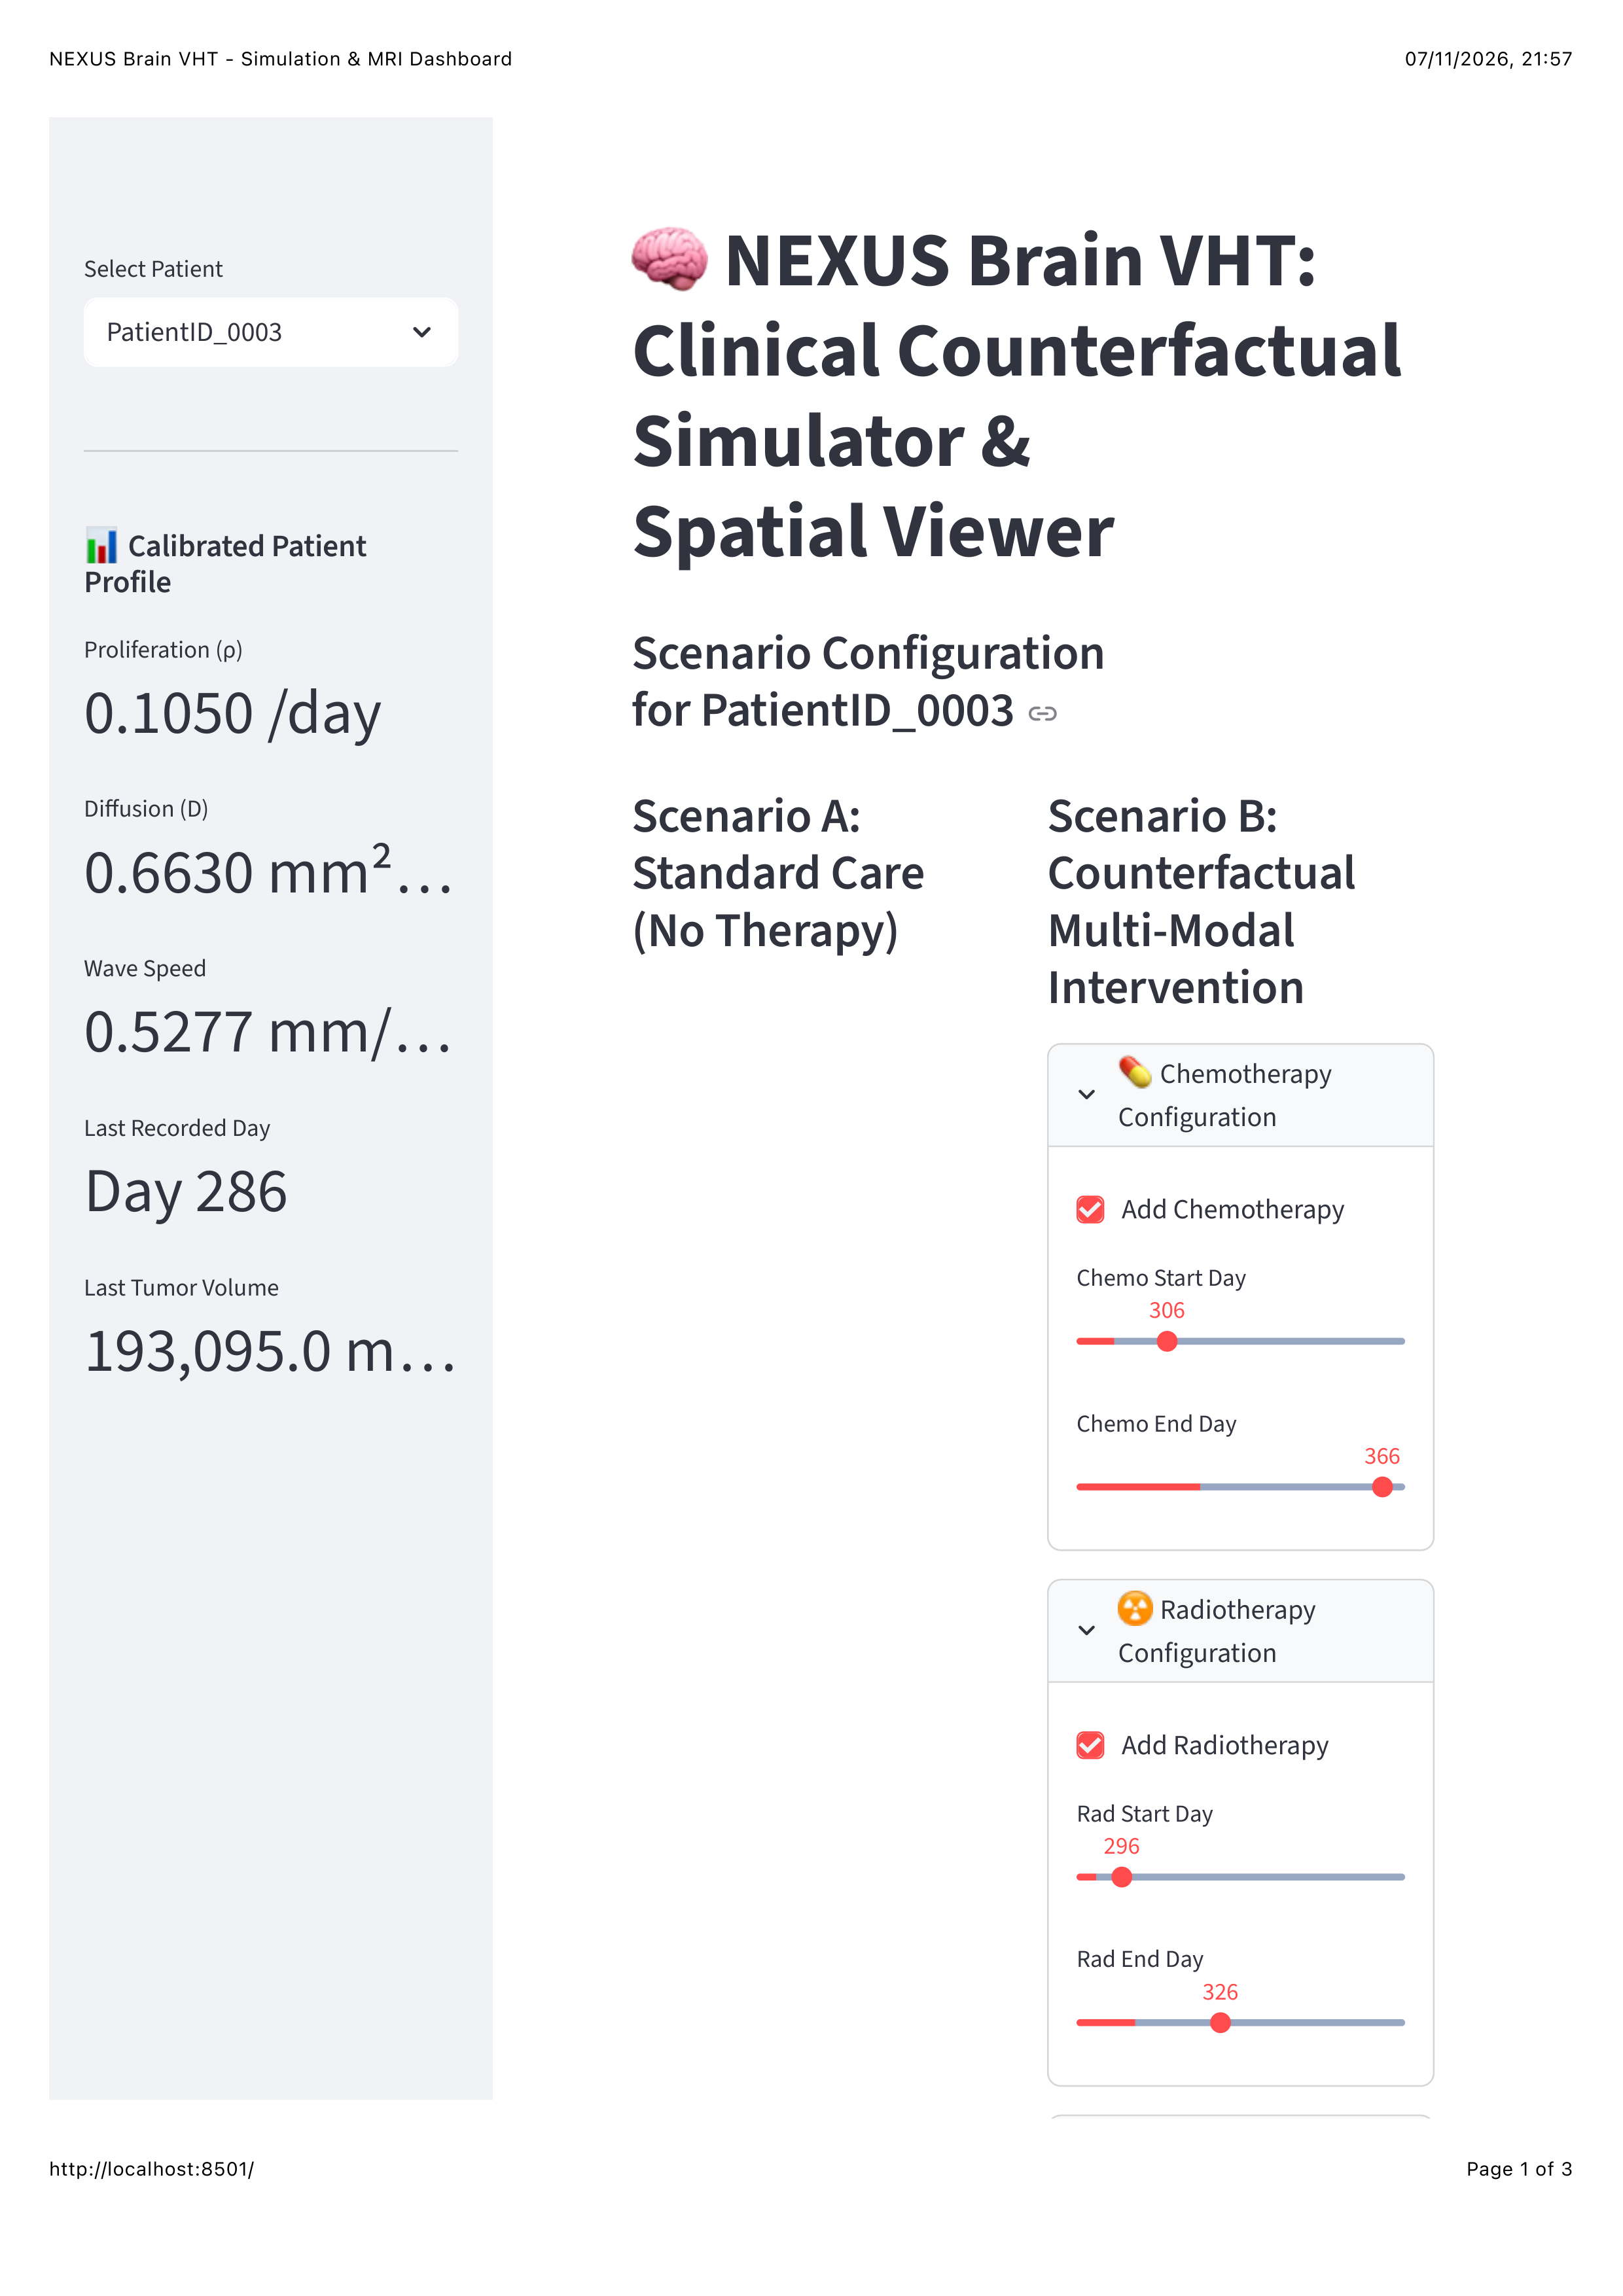
\includegraphics[width=0.70\textwidth]{figures/nexus_dashboard_page_1.png}
    \caption{NEXUS Brain VHT Dashboard — Page 1: Patient Profile and Scenario Configuration Controls.}
    \label{fig:dashboard_p1}
\end{figure}

\begin{figure}[htbp]
    \centering
    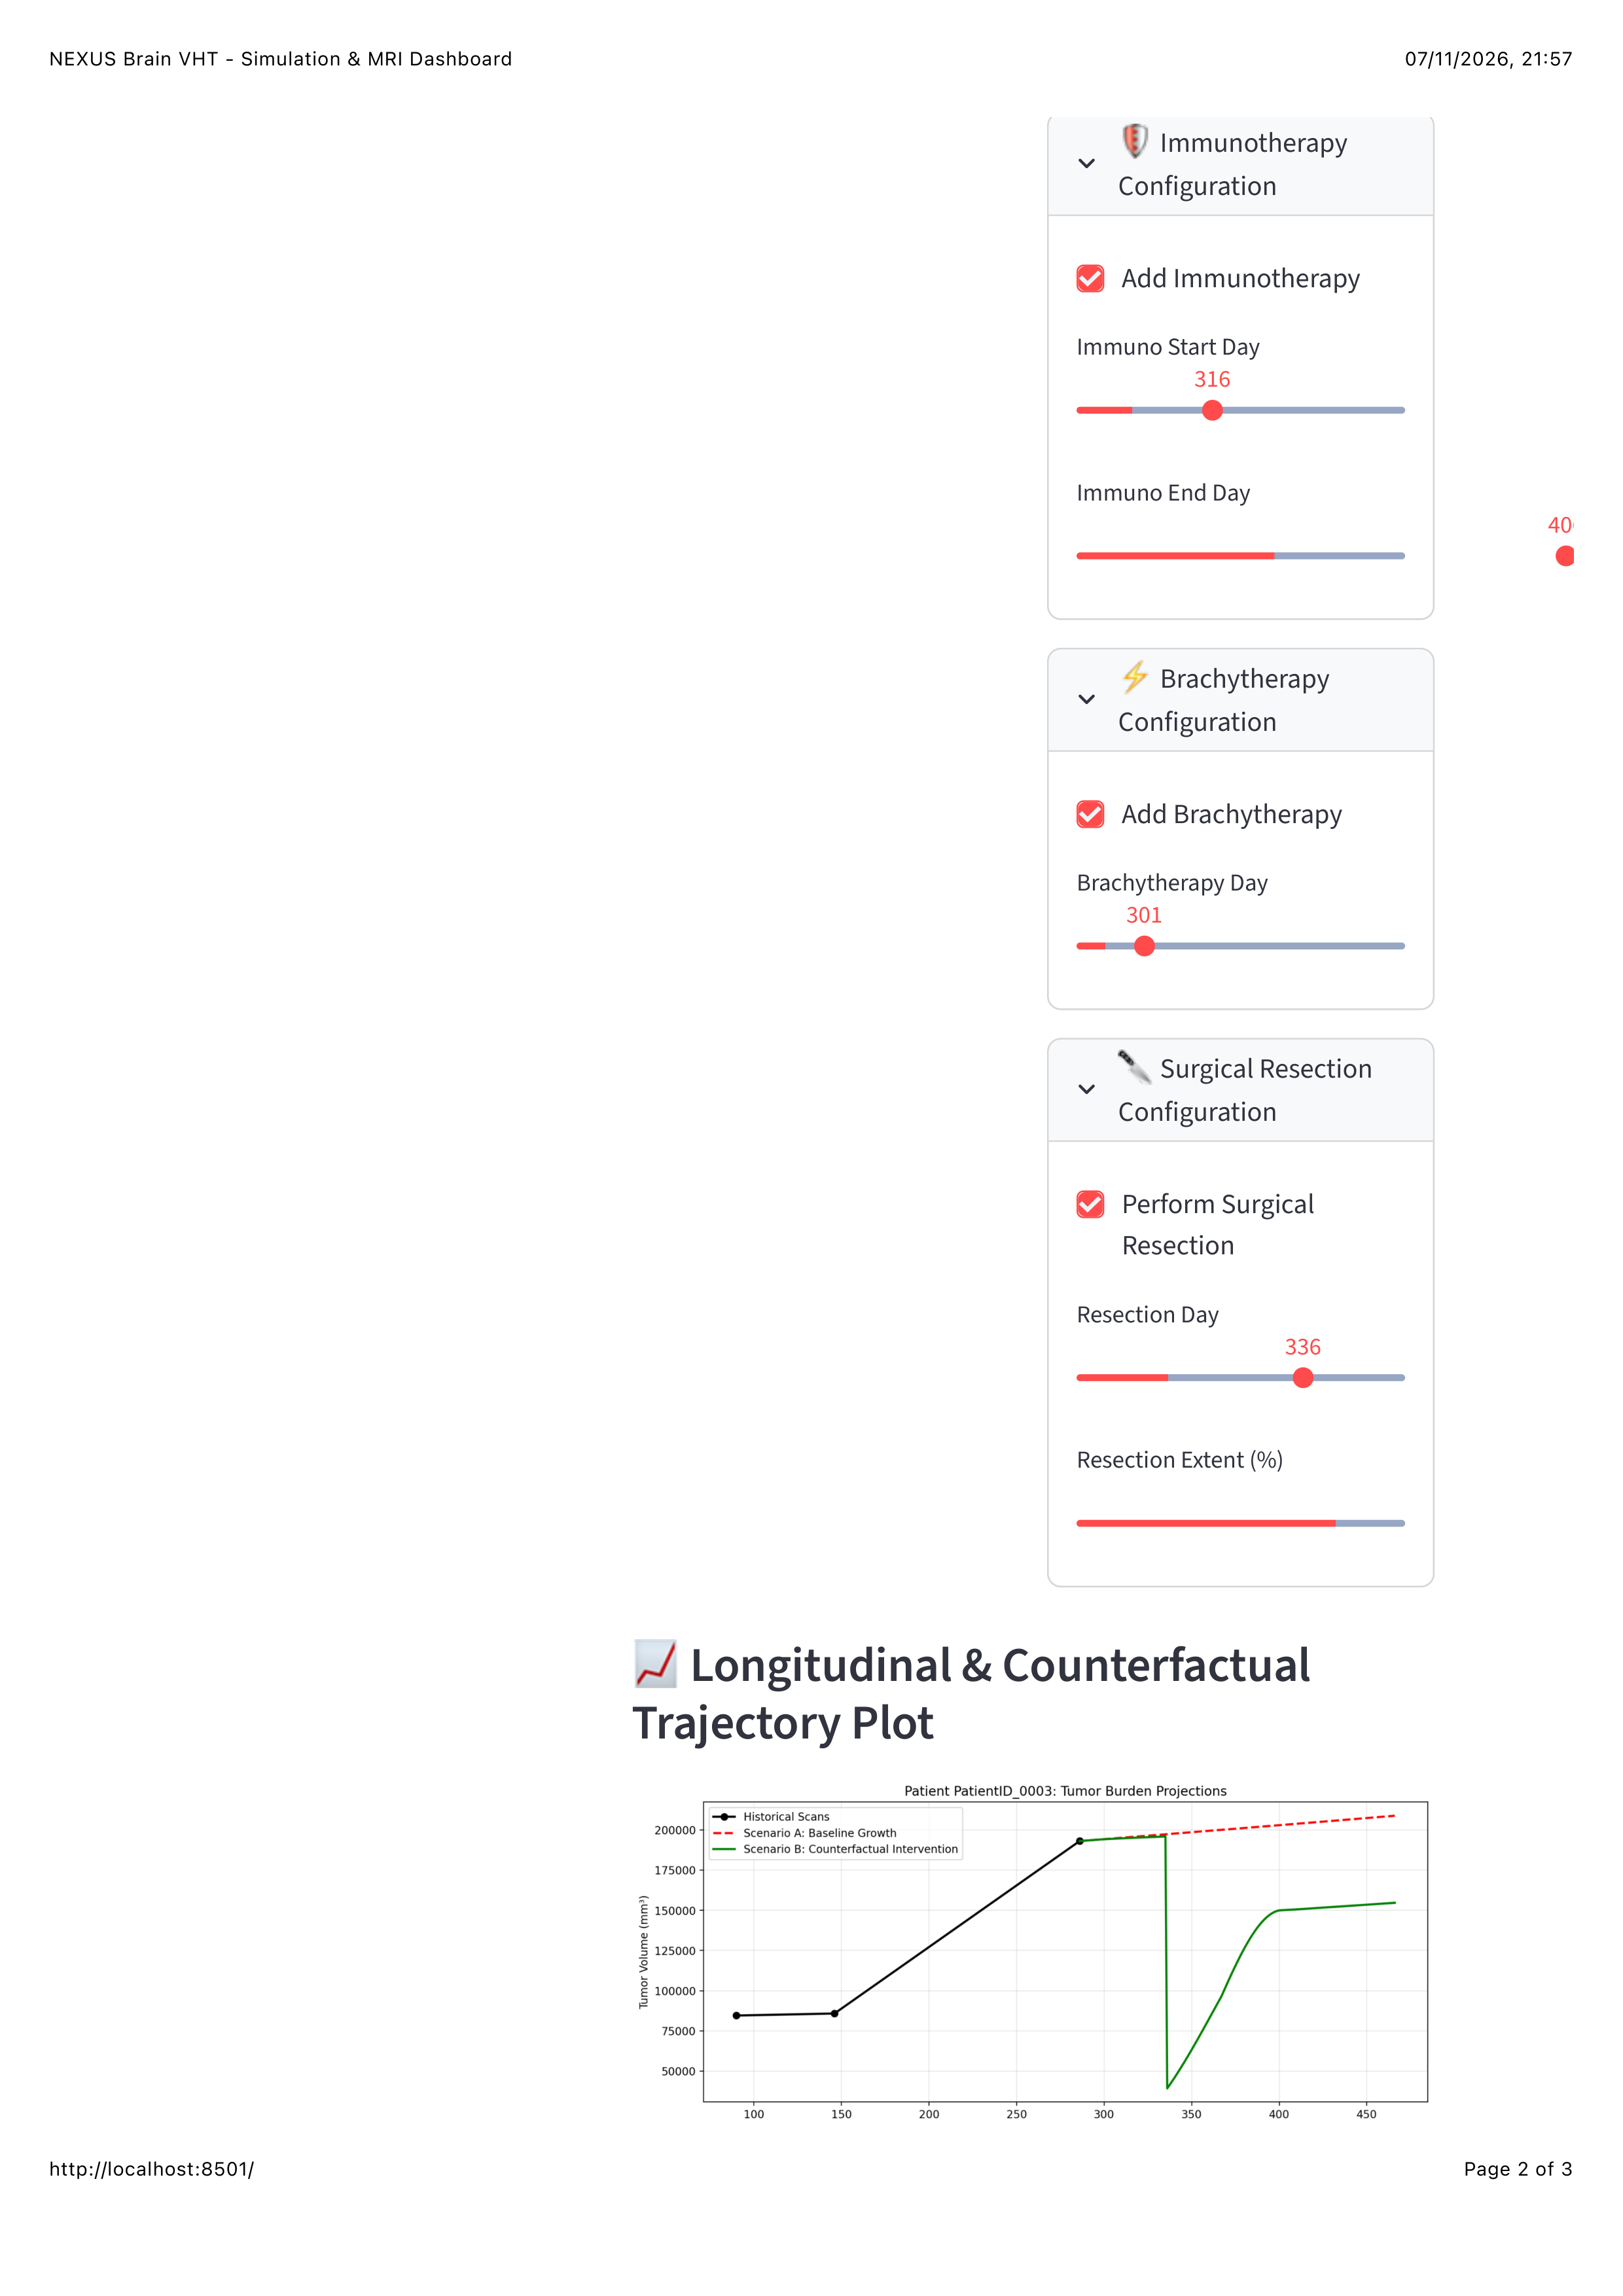
\includegraphics[width=0.85\textwidth]{figures/nexus_dashboard_page_2.png}
    \caption{NEXUS Brain VHT Dashboard — Page 2: Treatment Sliders and Longitudinal Counterfactual Plot.}
    \label{fig:dashboard_p2}
\end{figure}

\begin{figure}[htbp]
    \centering
    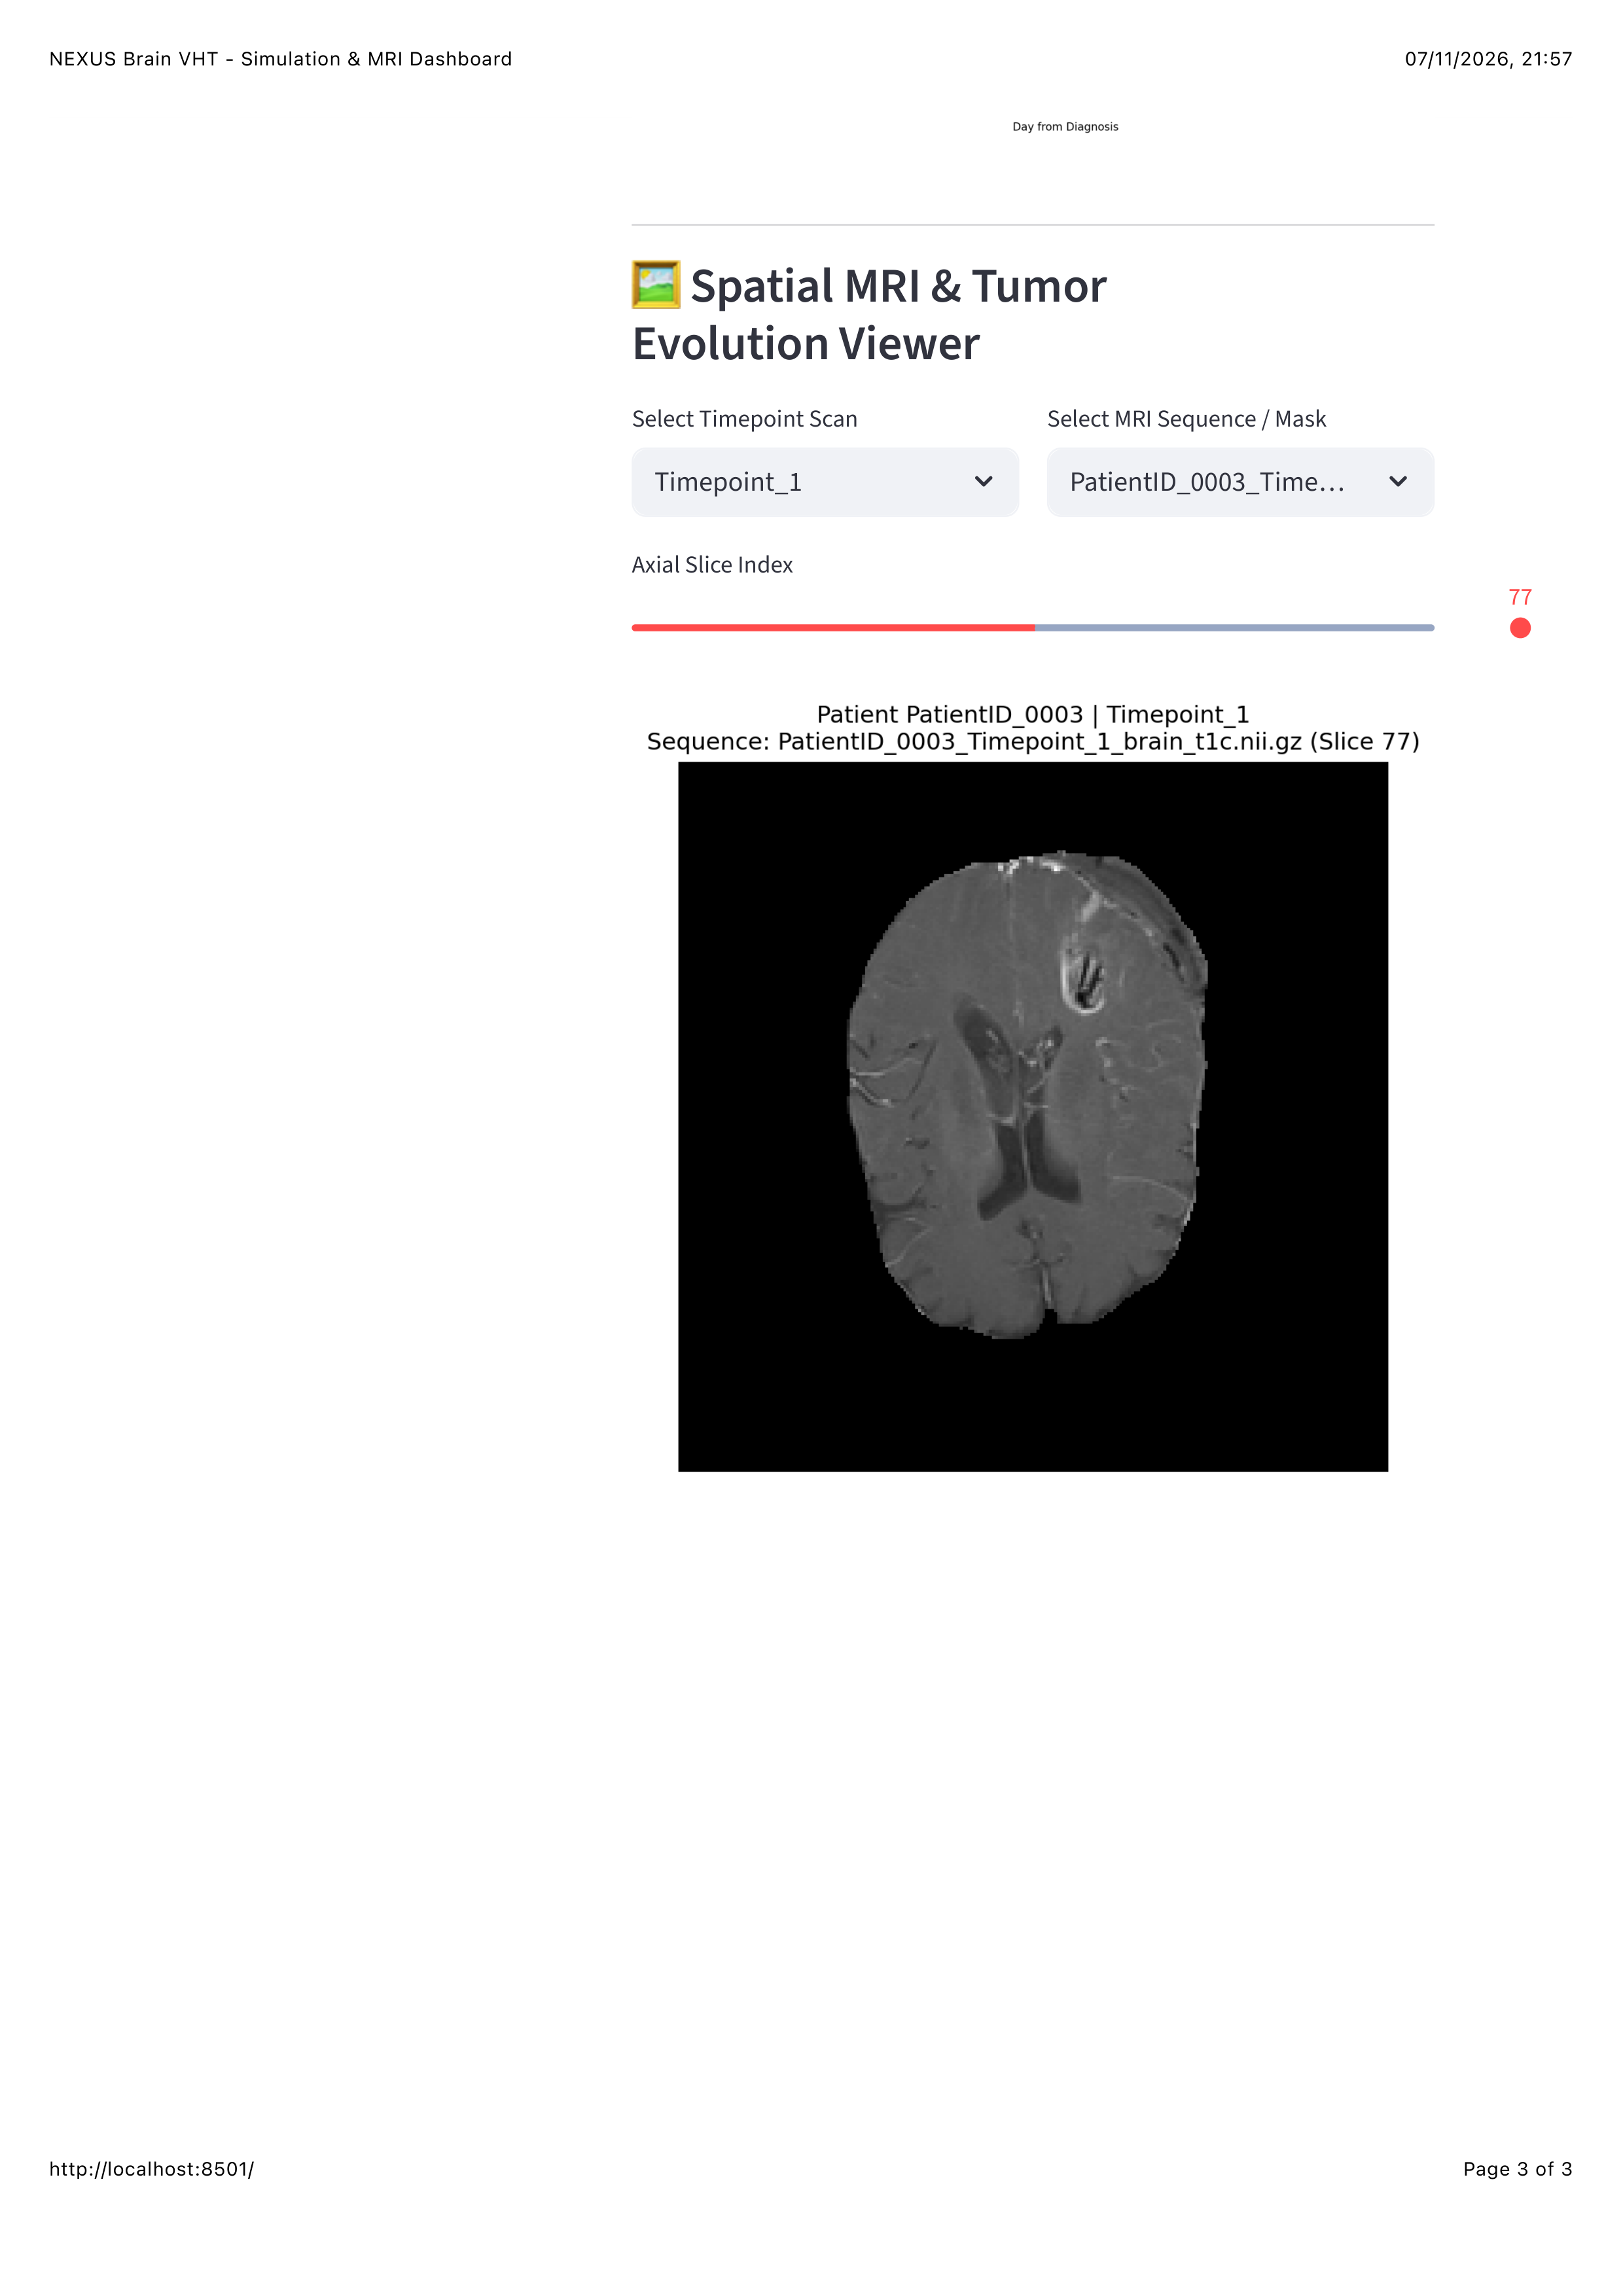
\includegraphics[width=0.85\textwidth]{figures/nexus_dashboard_page_3.png}
    \caption{NEXUS Brain VHT Dashboard — Page 3: Spatial NIfTI MRI Slice Viewer.}
    \label{fig:dashboard_p3}
\end{figure}

\newpage

%########################################################################


\addcontentsline{toc}{section}{References}
\bibliographystyle{unsrt}
\bibliography{biblio}

\end{document}
